\documentclass[12pt]{extarticle}
\usepackage[paperwidth=15in,paperheight=8.5in]{geometry}
\usepackage{amsmath}
\usepackage{hyperref}
\usepackage{multirow}
\usepackage{pdfpages}
\usepackage[utf8]{inputenc}
\title{Kaon mixing: chiral and continuum extrapolations}
\author{R Mukherjee}
\date{\today}
\begin{document}
\maketitle
\tableofcontents
\clearpage
\begin{figure}
\centering
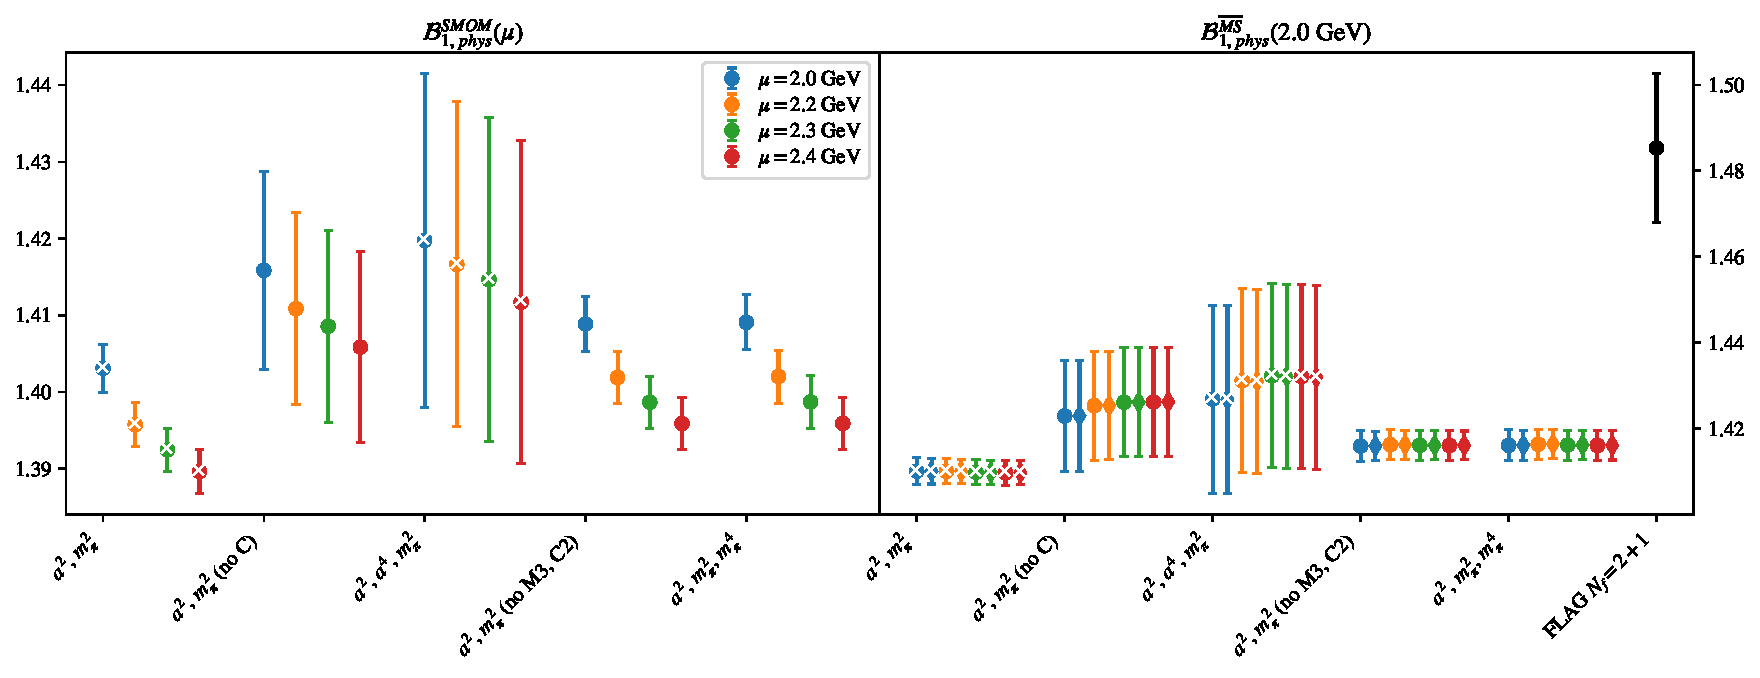
\includegraphics[page=1, width=1.1\textwidth]{VVpAA/SUSY/fit_summary_bag.pdf}
\caption{$\mathcal{B}_{1}$\\(left) $\mathcal{B}_{phys}$ in RI/SMOM scheme from fit variations (fits with $p$-value $<0.05$ marked with ``$\times$"). \\(right) $\mathcal{B}_{phys}$ in $\overline{MS}$ computed using $\mathcal{B}^{\overline{MS}} = R^{\overline{MS}\leftarrow SMOM}(2.0)\sigma_{npt}(2.0,\mu) \mathcal{B}^{SMOM}(\mu)$.}
\end{figure}
\clearpage
\begin{figure}
\centering
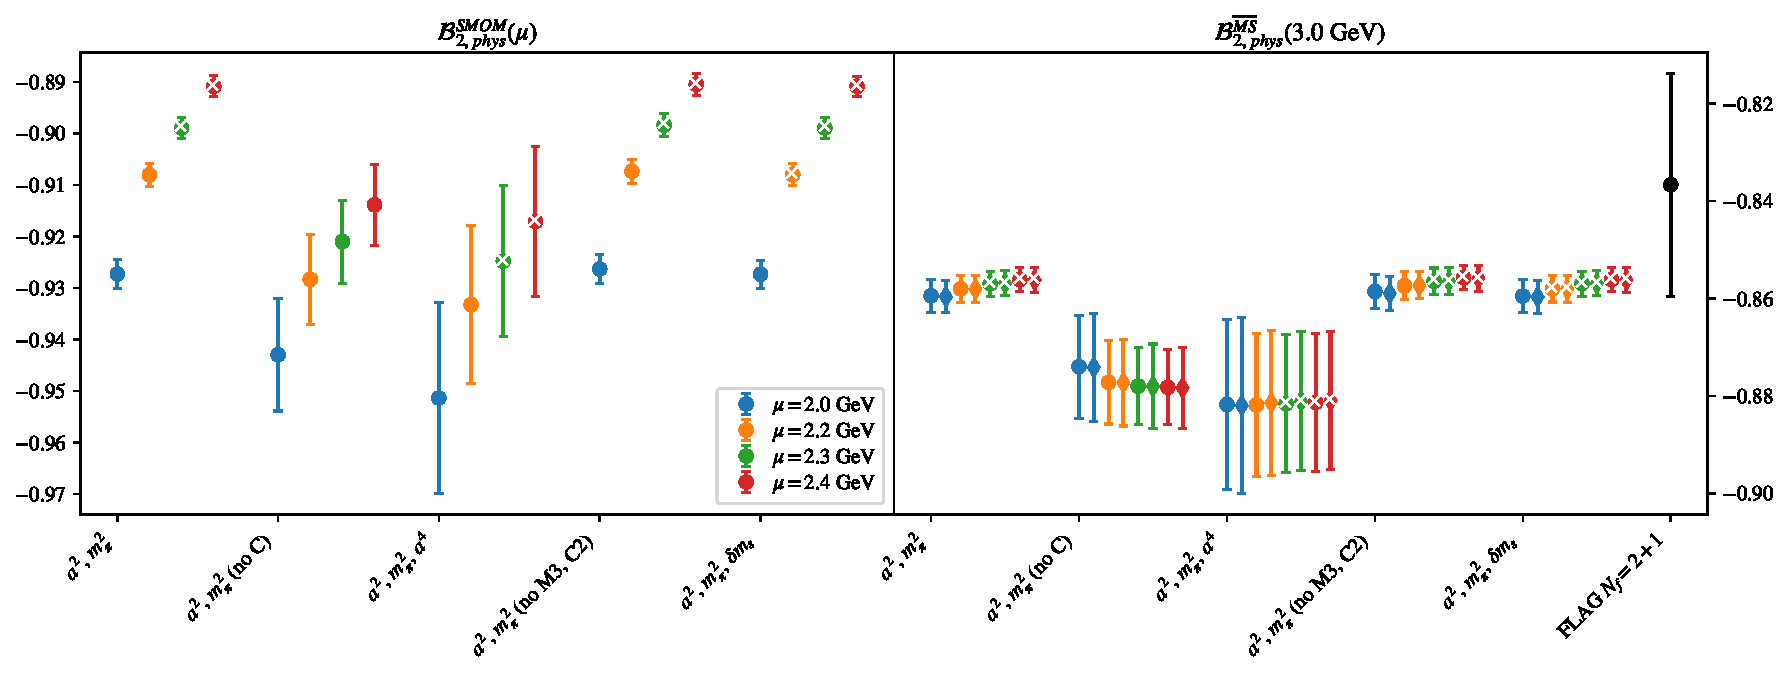
\includegraphics[page=1, width=1.1\textwidth]{VVmAA/SUSY/fit_summary_bag.pdf}
\caption{$\mathcal{B}_{2}$\\(left) $\mathcal{B}_{phys}$ in RI/SMOM scheme from fit variations (fits with $p$-value $<0.05$ marked with ``$\times$"). \\(right) $\mathcal{B}_{phys}$ in $\overline{MS}$ computed using $\mathcal{B}^{\overline{MS}} = R^{\overline{MS}\leftarrow SMOM}(3.0)\sigma_{npt}(3.0,\mu) \mathcal{B}^{SMOM}(\mu)$.}
\end{figure}
\clearpage
\begin{figure}
\centering
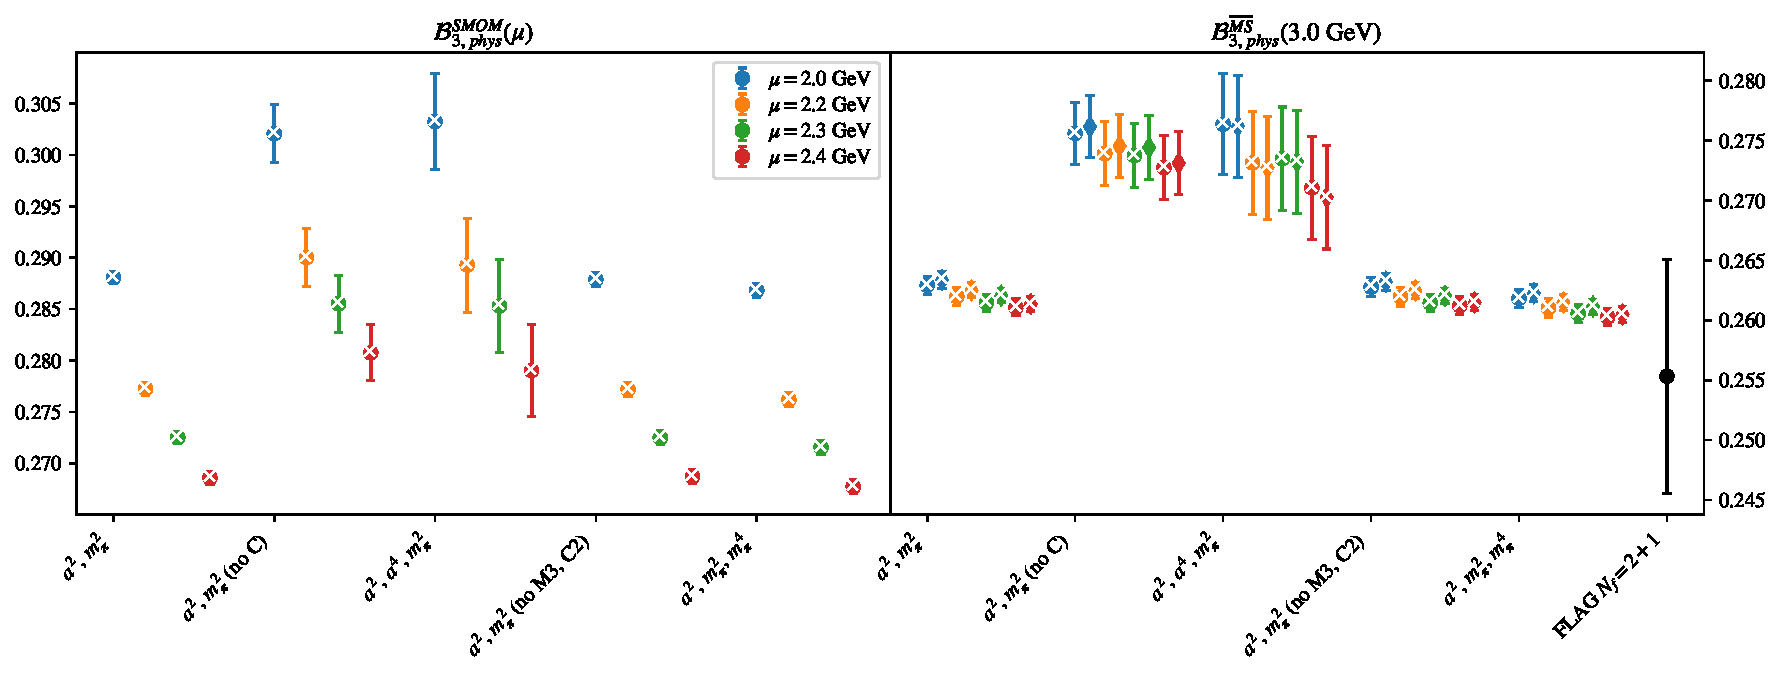
\includegraphics[page=1, width=1.1\textwidth]{SSmPP/SUSY/fit_summary_bag.pdf}
\caption{$\mathcal{B}_{3}$\\(left) $\mathcal{B}_{phys}$ in RI/SMOM scheme from fit variations (fits with $p$-value $<0.05$ marked with ``$\times$"). \\(right) $\mathcal{B}_{phys}$ in $\overline{MS}$ computed using $\mathcal{B}^{\overline{MS}} = R^{\overline{MS}\leftarrow SMOM}(3.0)\sigma_{npt}(3.0,\mu) \mathcal{B}^{SMOM}(\mu)$.}
\end{figure}
\clearpage
\begin{figure}
\centering
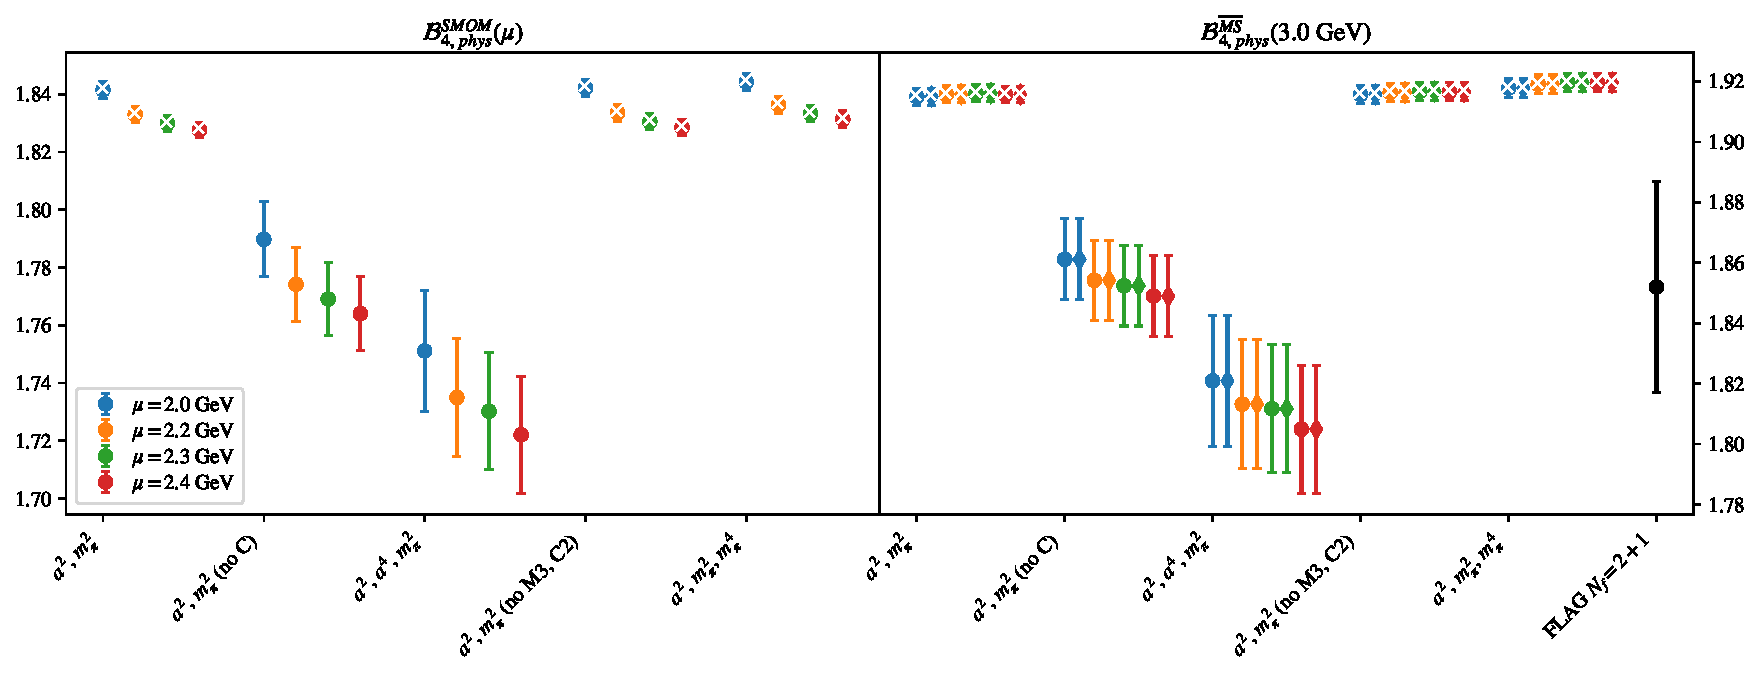
\includegraphics[page=1, width=1.1\textwidth]{SSpPP/SUSY/fit_summary_bag.pdf}
\caption{$\mathcal{B}_{4}$\\(left) $\mathcal{B}_{phys}$ in RI/SMOM scheme from fit variations (fits with $p$-value $<0.05$ marked with ``$\times$"). \\(right) $\mathcal{B}_{phys}$ in $\overline{MS}$ computed using $\mathcal{B}^{\overline{MS}} = R^{\overline{MS}\leftarrow SMOM}(3.0)\sigma_{npt}(3.0,\mu) \mathcal{B}^{SMOM}(\mu)$.}
\end{figure}
\clearpage
\begin{figure}
\centering
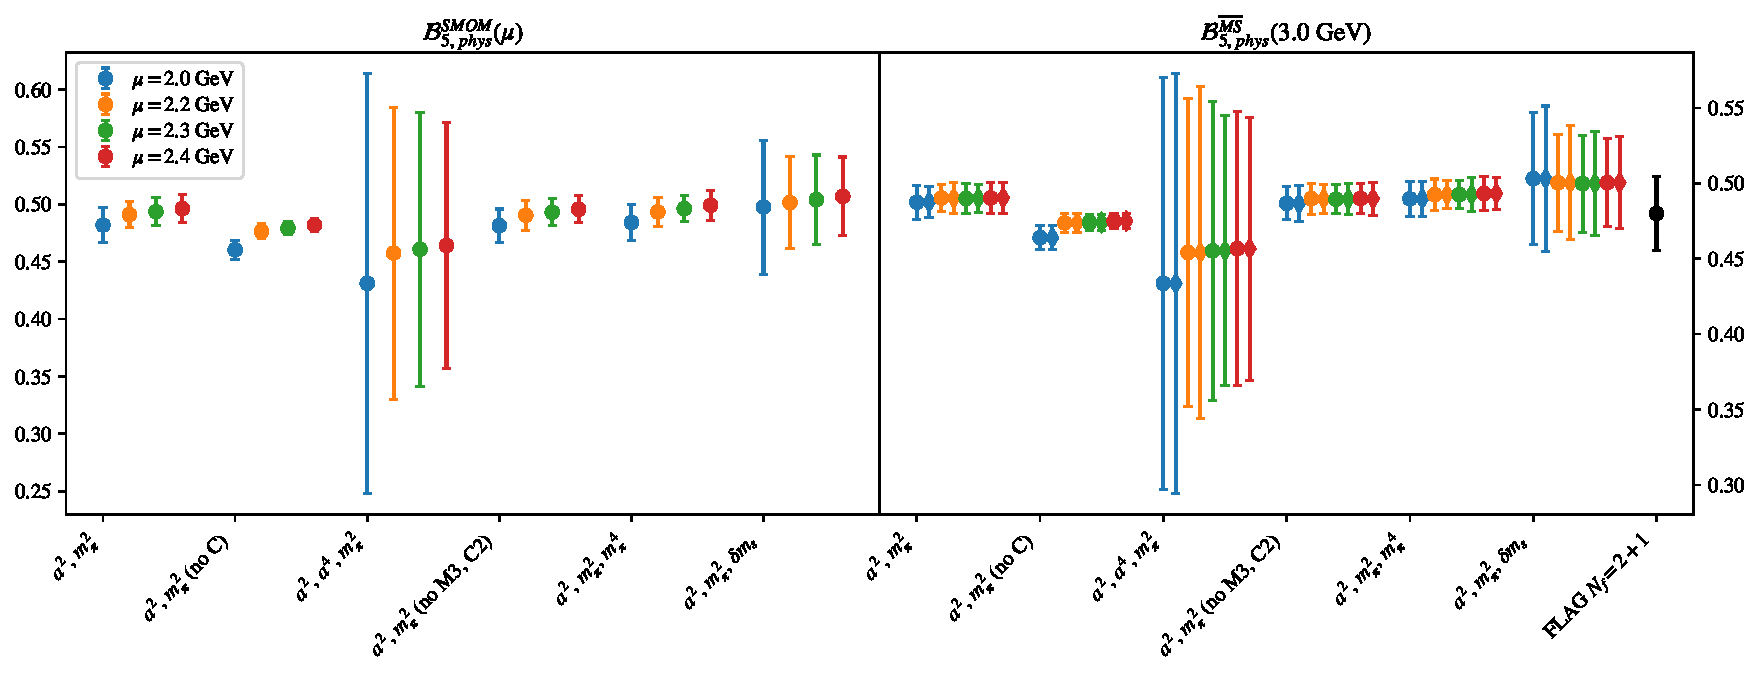
\includegraphics[page=1, width=1.1\textwidth]{TT/SUSY/fit_summary_bag.pdf}
\caption{$\mathcal{B}_{5}$\\(left) $\mathcal{B}_{phys}$ in RI/SMOM scheme from fit variations (fits with $p$-value $<0.05$ marked with ``$\times$"). \\(right) $\mathcal{B}_{phys}$ in $\overline{MS}$ computed using $\mathcal{B}^{\overline{MS}} = R^{\overline{MS}\leftarrow SMOM}(3.0)\sigma_{npt}(3.0,\mu) \mathcal{B}^{SMOM}(\mu)$.}
\end{figure}
\clearpage
\section{$\mathcal{B}_1$}
\begin{table}[h!]
\begin{center}
\begin{tabular}{|c|c|c|c|c|c|}
\hline
$\mu$ (GeV) & $a^2$, $m_\pi^2$& $a^2$, $m_\pi^2$ (no C)& $a^2$, $m_\pi^2$, $a^4$& $a^2$, $m_\pi^2$ (no M3, C2)& $a^2$, $m_\pi^2$, $\delta m_s$\\
\hline
2.0& \hyperlink{VVpAA/SUSY/bag_a2m2_20.pdf.1}{\textbf{1.4010(29)}: 2.701 (0.019)} & \hyperlink{VVpAA/SUSY/bag_a2m2noC_20.pdf.1}{\textbf{1.435(12)}: 0.271 (0.763)} & \hyperlink{VVpAA/SUSY/bag_a2a4m2_20.pdf.1}{\textbf{1.451(22)}: 2.04 (0.086)} & \hyperlink{VVpAA/SUSY/bag_a2m2mcut_20.pdf.1}{\textbf{1.4051(33)}: 2.159 (0.091)} & \hyperlink{VVpAA/SUSY/bag_a2m2delm_20.pdf.1}{\textbf{1.4012(29)}: 1.362 (0.244)}\\
2.2& \hyperlink{VVpAA/SUSY/bag_a2m2_22.pdf.1}{\textbf{1.3935(29)}: 3.208 (0.007)} & \hyperlink{VVpAA/SUSY/bag_a2m2noC_22.pdf.1}{\textbf{1.431(12)}: 0.309 (0.734)} & \hyperlink{VVpAA/SUSY/bag_a2a4m2_22.pdf.1}{\textbf{1.450(22)}: 2.298 (0.056)} & \hyperlink{VVpAA/SUSY/bag_a2m2mcut_22.pdf.1}{\textbf{1.3979(33)}: 2.579 (0.052)} & \hyperlink{VVpAA/SUSY/bag_a2m2delm_22.pdf.1}{\textbf{1.3938(29)}: 1.436 (0.219)}\\
2.3& \hyperlink{VVpAA/SUSY/bag_a2m2_23.pdf.1}{\textbf{1.3900(28)}: 3.454 (0.004)} & \hyperlink{VVpAA/SUSY/bag_a2m2noC_23.pdf.1}{\textbf{1.429(12)}: 0.327 (0.721)} & \hyperlink{VVpAA/SUSY/bag_a2a4m2_23.pdf.1}{\textbf{1.449(22)}: 2.461 (0.043)} & \hyperlink{VVpAA/SUSY/bag_a2m2mcut_23.pdf.1}{\textbf{1.3946(32)}: 2.832 (0.037)} & \hyperlink{VVpAA/SUSY/bag_a2m2delm_23.pdf.1}{\textbf{1.3903(28)}: 1.559 (0.182)}\\
2.4& \hyperlink{VVpAA/SUSY/bag_a2m2_24.pdf.1}{\textbf{1.3870(29)}: 3.491 (0.004)} & \hyperlink{VVpAA/SUSY/bag_a2m2noC_24.pdf.1}{\textbf{1.426(12)}: 0.336 (0.714)} & \hyperlink{VVpAA/SUSY/bag_a2a4m2_24.pdf.1}{\textbf{1.446(22)}: 2.543 (0.038)} & \hyperlink{VVpAA/SUSY/bag_a2m2mcut_24.pdf.1}{\textbf{1.3916(33)}: 2.825 (0.037)} & \hyperlink{VVpAA/SUSY/bag_a2m2delm_24.pdf.1}{\textbf{1.3874(29)}: 1.603 (0.17)}\\
\hline
\end{tabular}
\caption{Physical point value from chiral and continuum extrapolation at renormalisation scale $\mu$. Entries are \textbf{value(error)}: $\chi^2/\text{DOF}$ ($p$-value).}
\end{center}
\end{table}
\begin{table}[h!]
\begin{center}
\begin{tabular}{|c c|c|c|c|c|c|}
\hline
$\mu$ (GeV) &  & $a^2$, $m_\pi^2$& $a^2$, $m_\pi^2$ (no C)& $a^2$, $m_\pi^2$, $a^4$& $a^2$, $m_\pi^2$ (no M3, C2)& $a^2$, $m_\pi^2$, $\delta m_s$\\
\hline
\multirow{3}{0.5in}{2.0} & $\alpha$ & 0.143(10)& -0.048(75)& -0.32(20)& 0.131(11)& 0.147(10)\\
 & $\beta$ & 0.00410(23)& 0.00347(41)& 0.00437(25)& 0.00345(36)& 0.00538(50)\\
 & $\gamma$ &  &  & 0.95(42)&  & -0.049(16)\\
\hline
\multirow{3}{0.5in}{2.2} & $\alpha$ & 0.149(10)& -0.062(75)& -0.38(20)& 0.135(11)& 0.153(10)\\
 & $\beta$ & 0.00399(22)& 0.00334(40)& 0.00429(25)& 0.00327(35)& 0.00540(48)\\
 & $\gamma$ &  &  & 1.07(42)&  & -0.055(16)\\
\hline
\multirow{3}{0.5in}{2.3} & $\alpha$ & 0.152(10)& -0.068(75)& -0.39(20)& 0.138(11)& 0.155(10)\\
 & $\beta$ & 0.00395(22)& 0.00328(41)& 0.00427(25)& 0.00322(36)& 0.00541(49)\\
 & $\gamma$ &  &  & 1.11(42)&  & -0.056(16)\\
\hline
\multirow{3}{0.5in}{2.4} & $\alpha$ & 0.153(10)& -0.068(76)& -0.39(20)& 0.138(11)& 0.156(10)\\
 & $\beta$ & 0.00395(22)& 0.00325(40)& 0.00426(25)& 0.00320(35)& 0.00540(49)\\
 & $\gamma$ &  &  & 1.11(42)&  & -0.056(16)\\
\hline
\end{tabular}
\caption{Fit values of coefficients in $Q = Q_{phys} + \mathbf{\alpha} a^2 + \mathbf{\beta}\left(\frac{m_\pi^2}{f_\pi^2}-\frac{m_{\pi,PDG}^2}{f_\pi^2}\right) + \gamma(\ldots)$}
\end{center}
\end{table}
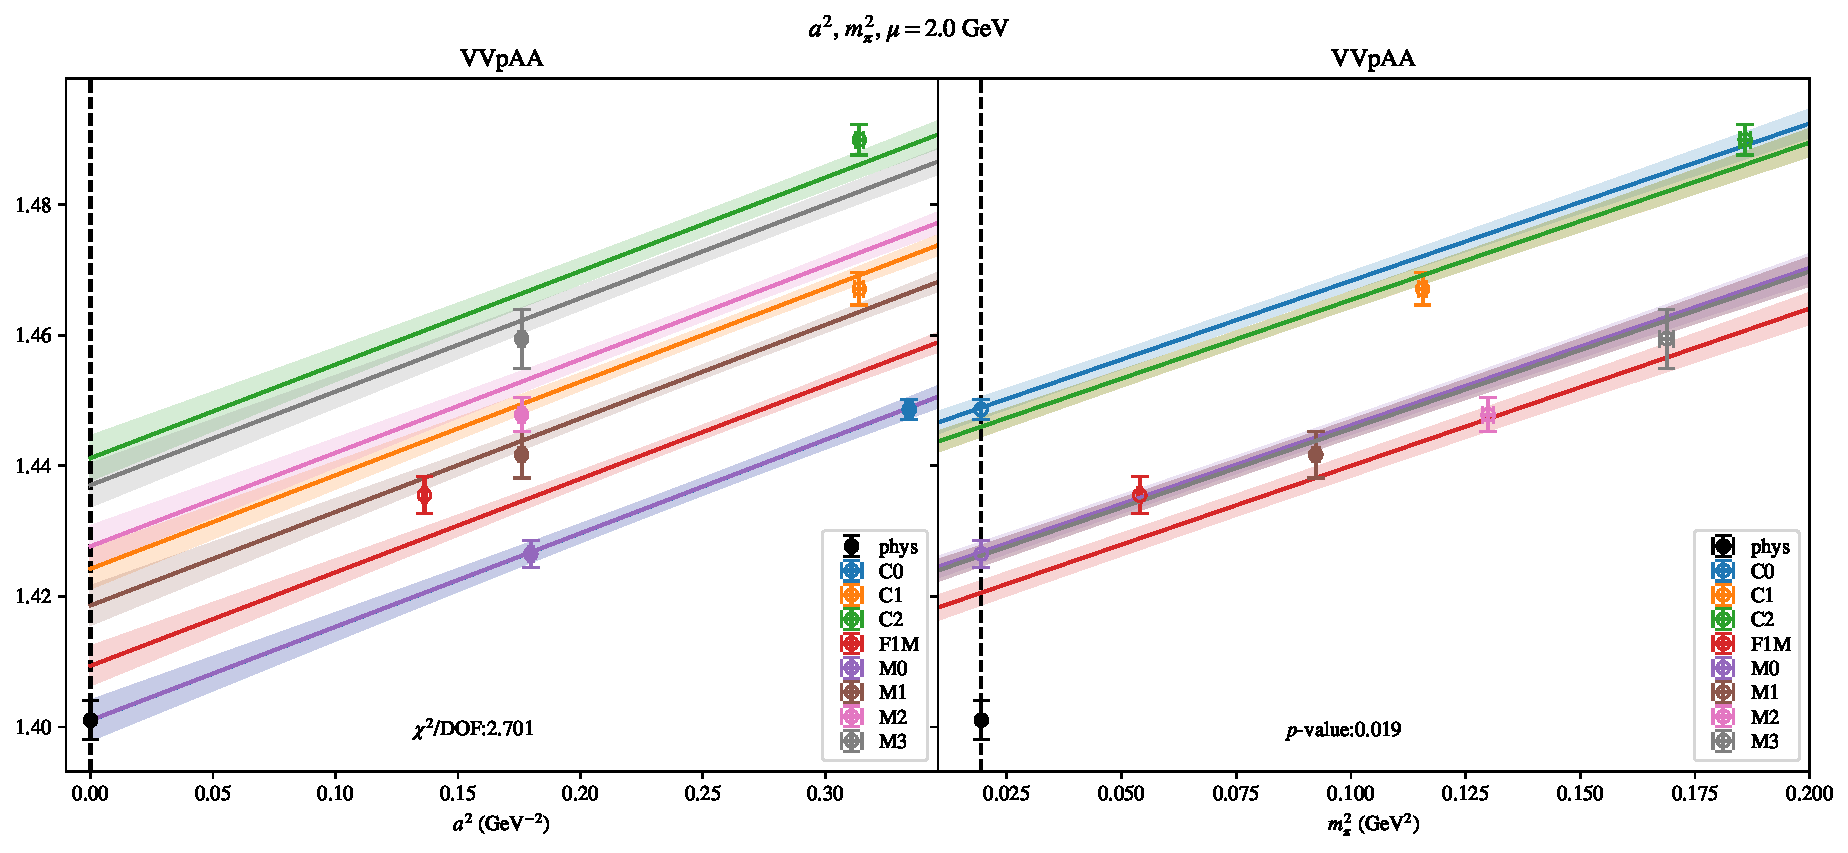
\includepdf[link, pages=-]{VVpAA/SUSY/bag_a2m2_20.pdf}
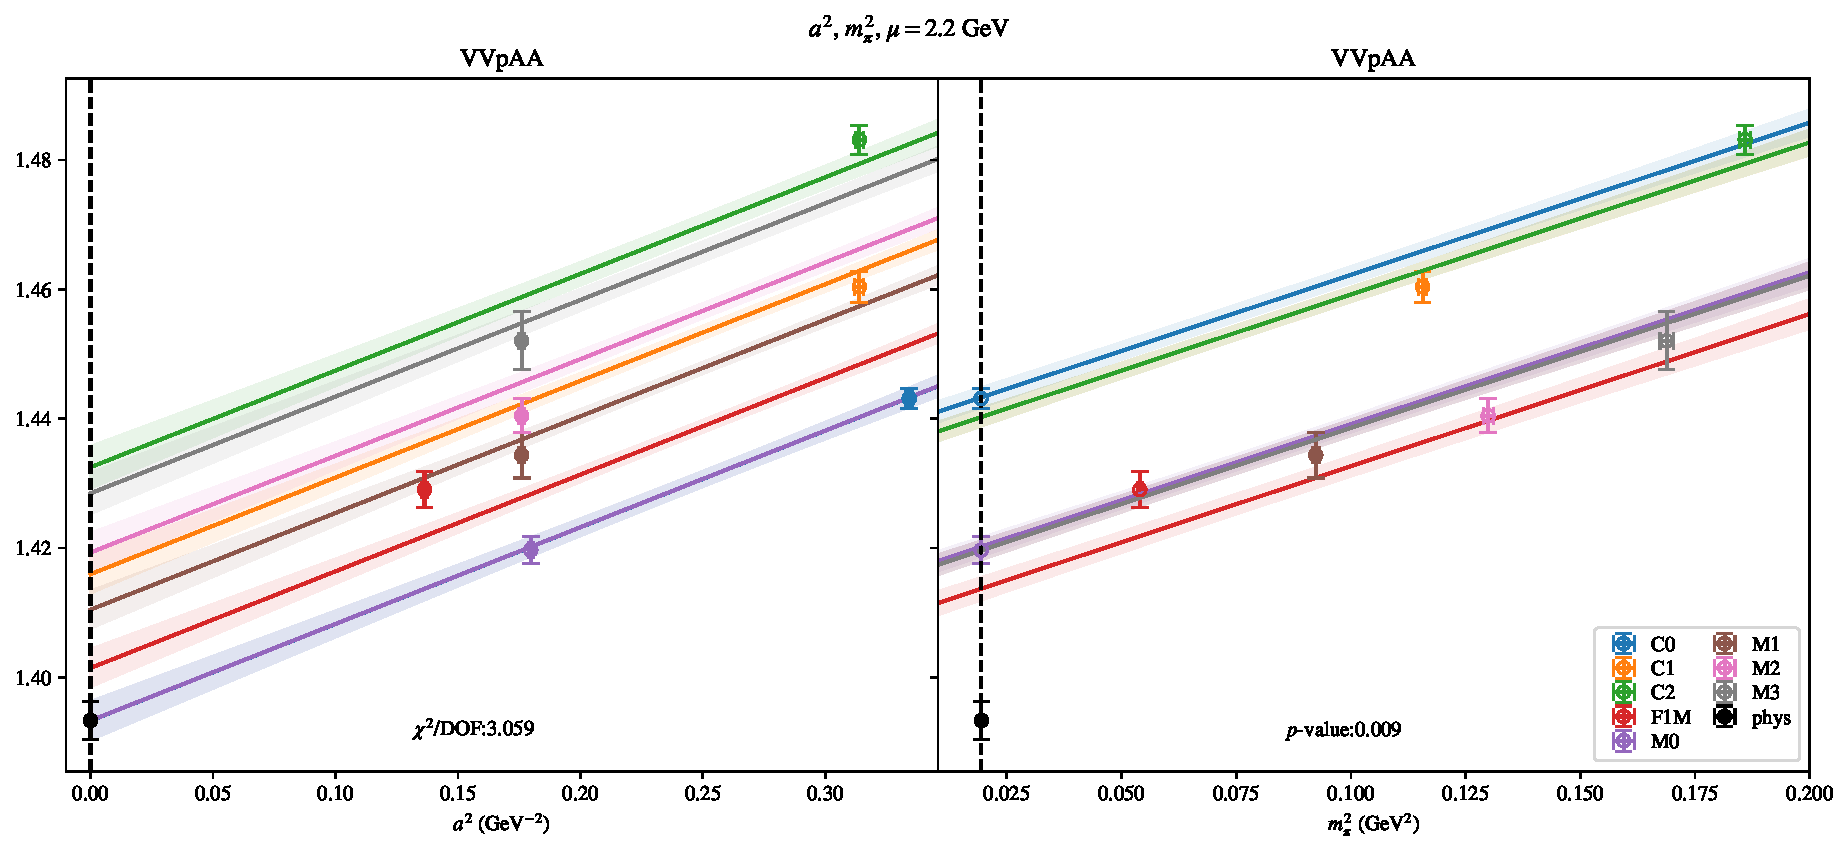
\includepdf[link, pages=-]{VVpAA/SUSY/bag_a2m2_22.pdf}
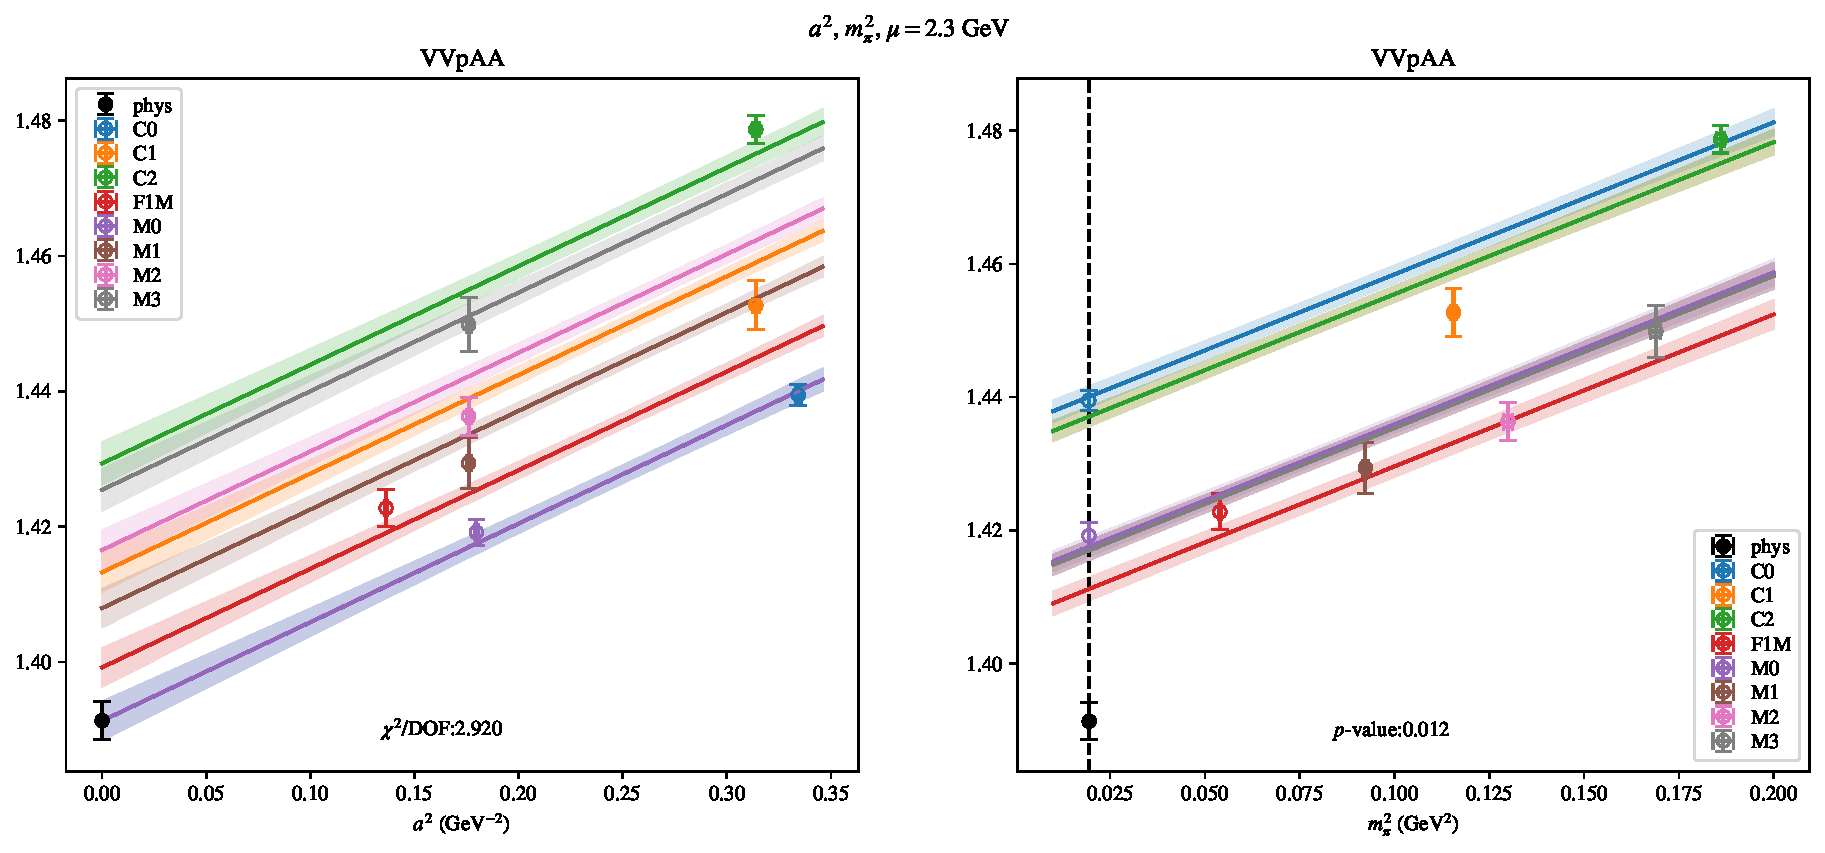
\includepdf[link, pages=-]{VVpAA/SUSY/bag_a2m2_23.pdf}
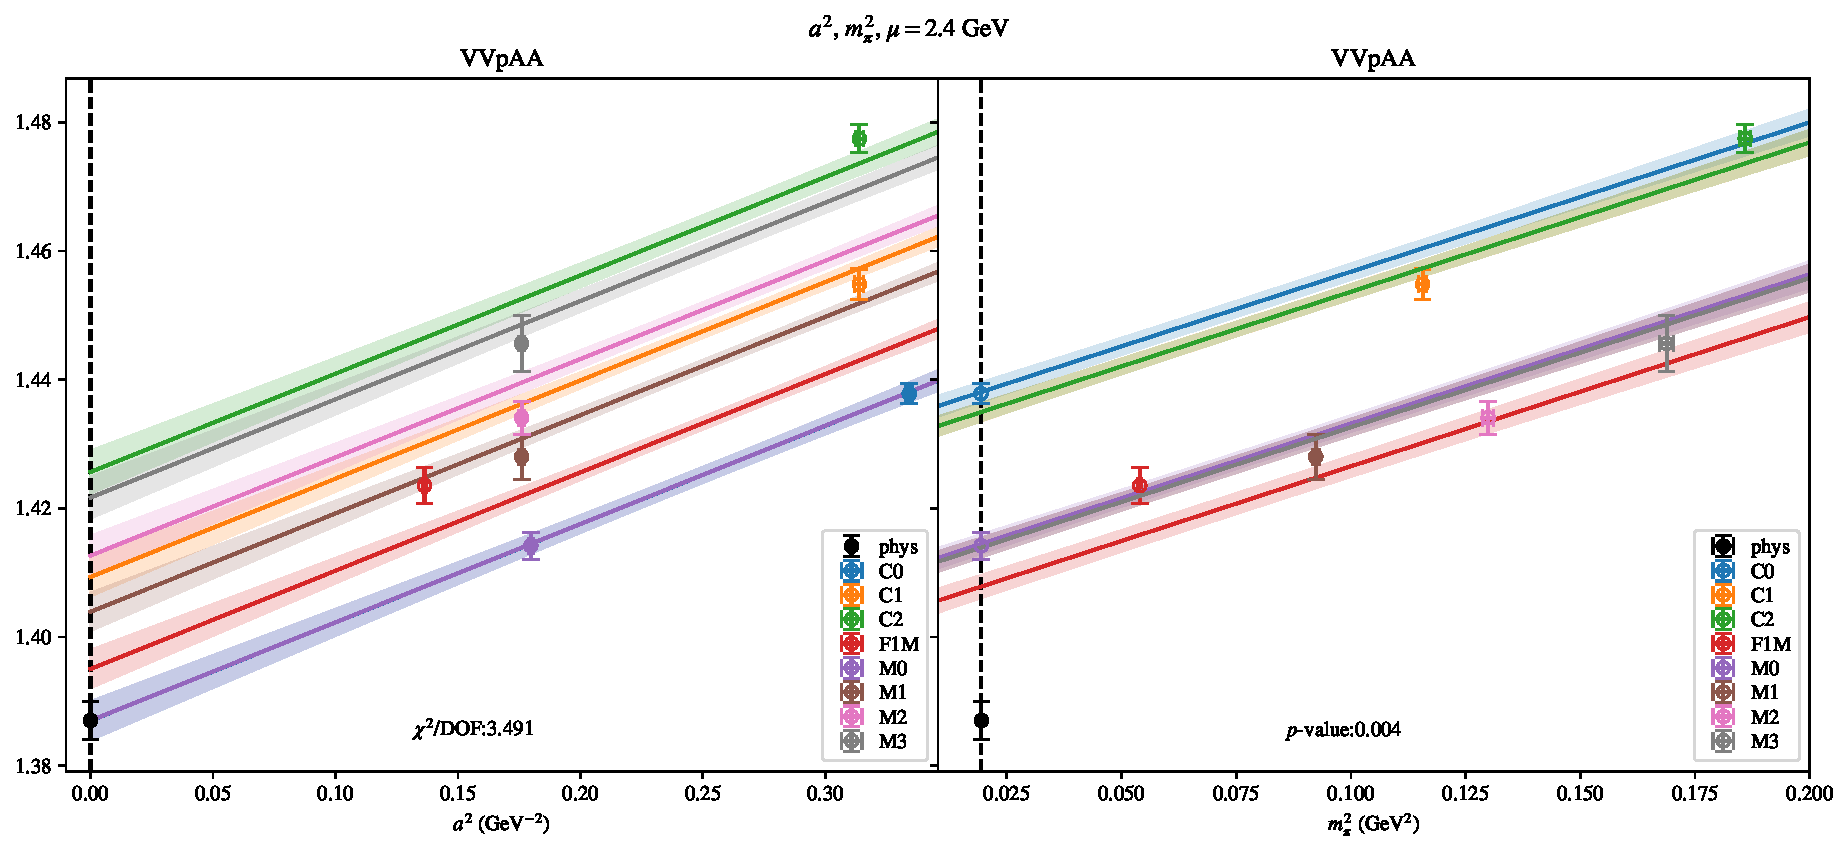
\includepdf[link, pages=-]{VVpAA/SUSY/bag_a2m2_24.pdf}
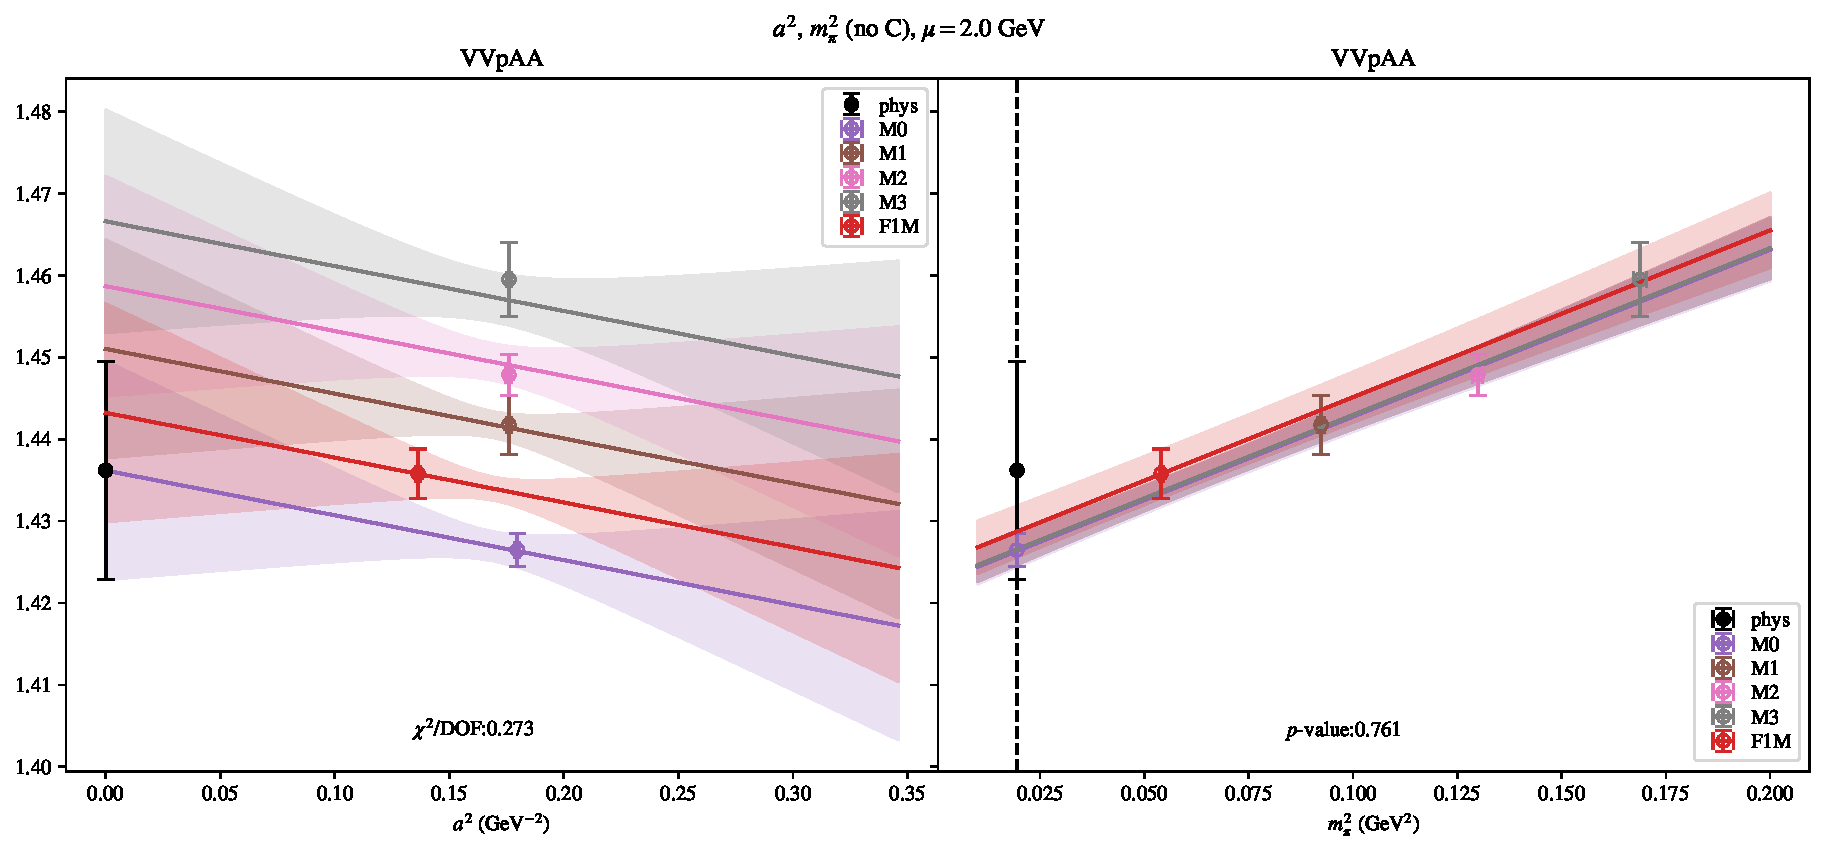
\includepdf[link, pages=-]{VVpAA/SUSY/bag_a2m2noC_20.pdf}
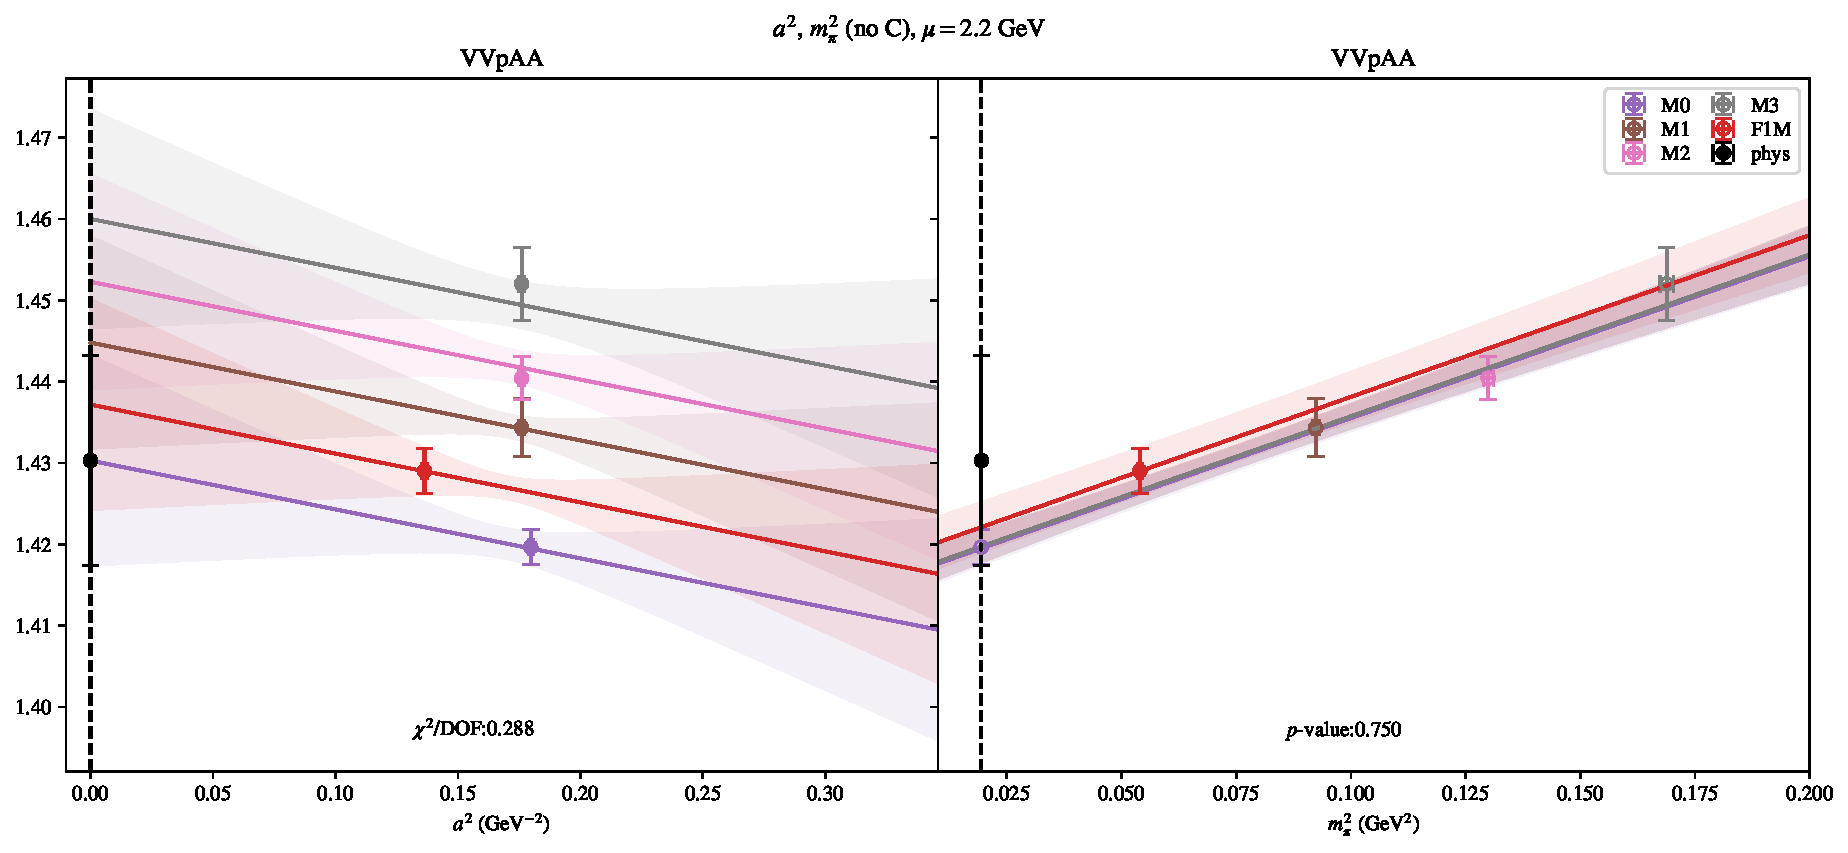
\includepdf[link, pages=-]{VVpAA/SUSY/bag_a2m2noC_22.pdf}
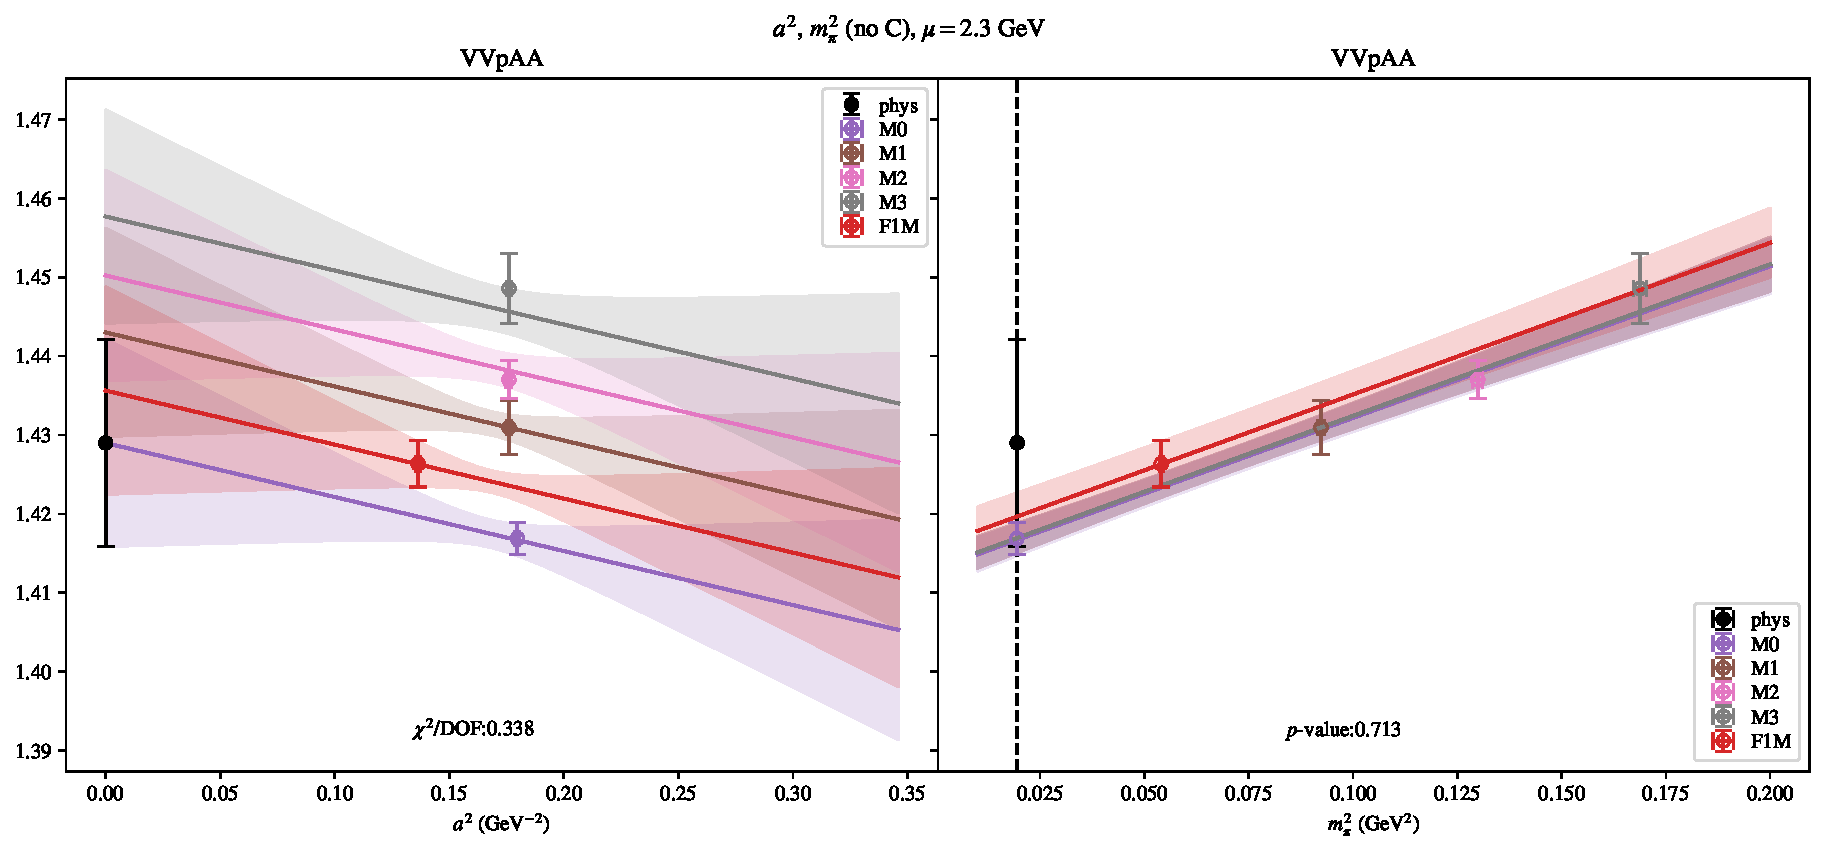
\includepdf[link, pages=-]{VVpAA/SUSY/bag_a2m2noC_23.pdf}
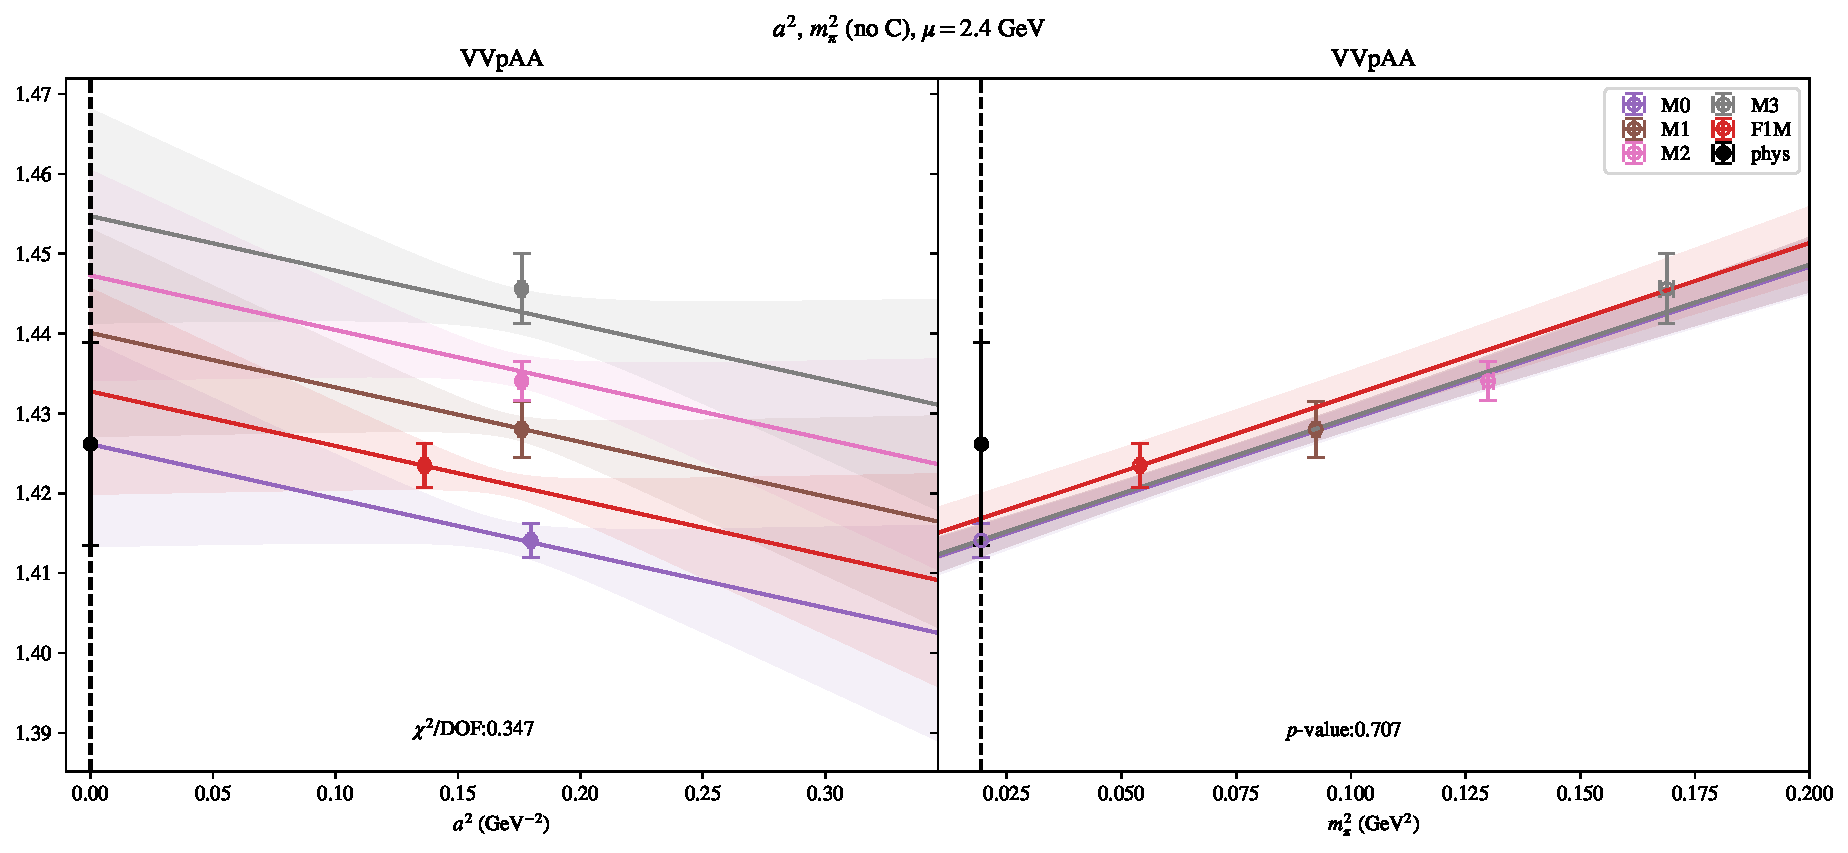
\includepdf[link, pages=-]{VVpAA/SUSY/bag_a2m2noC_24.pdf}
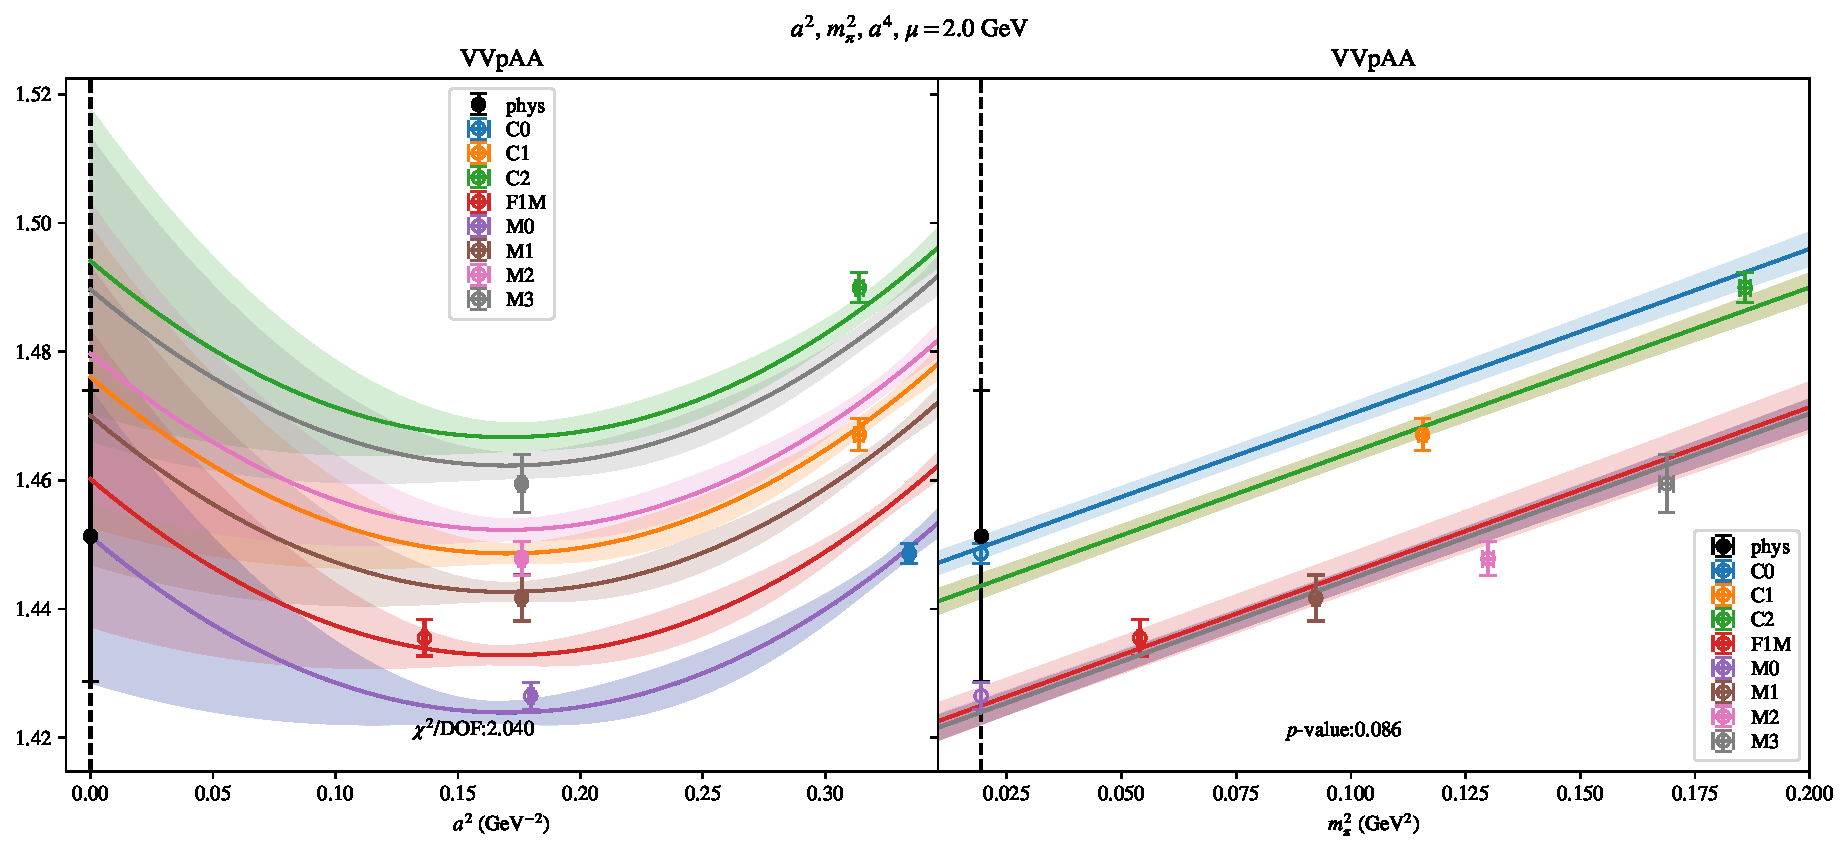
\includepdf[link, pages=-]{VVpAA/SUSY/bag_a2a4m2_20.pdf}
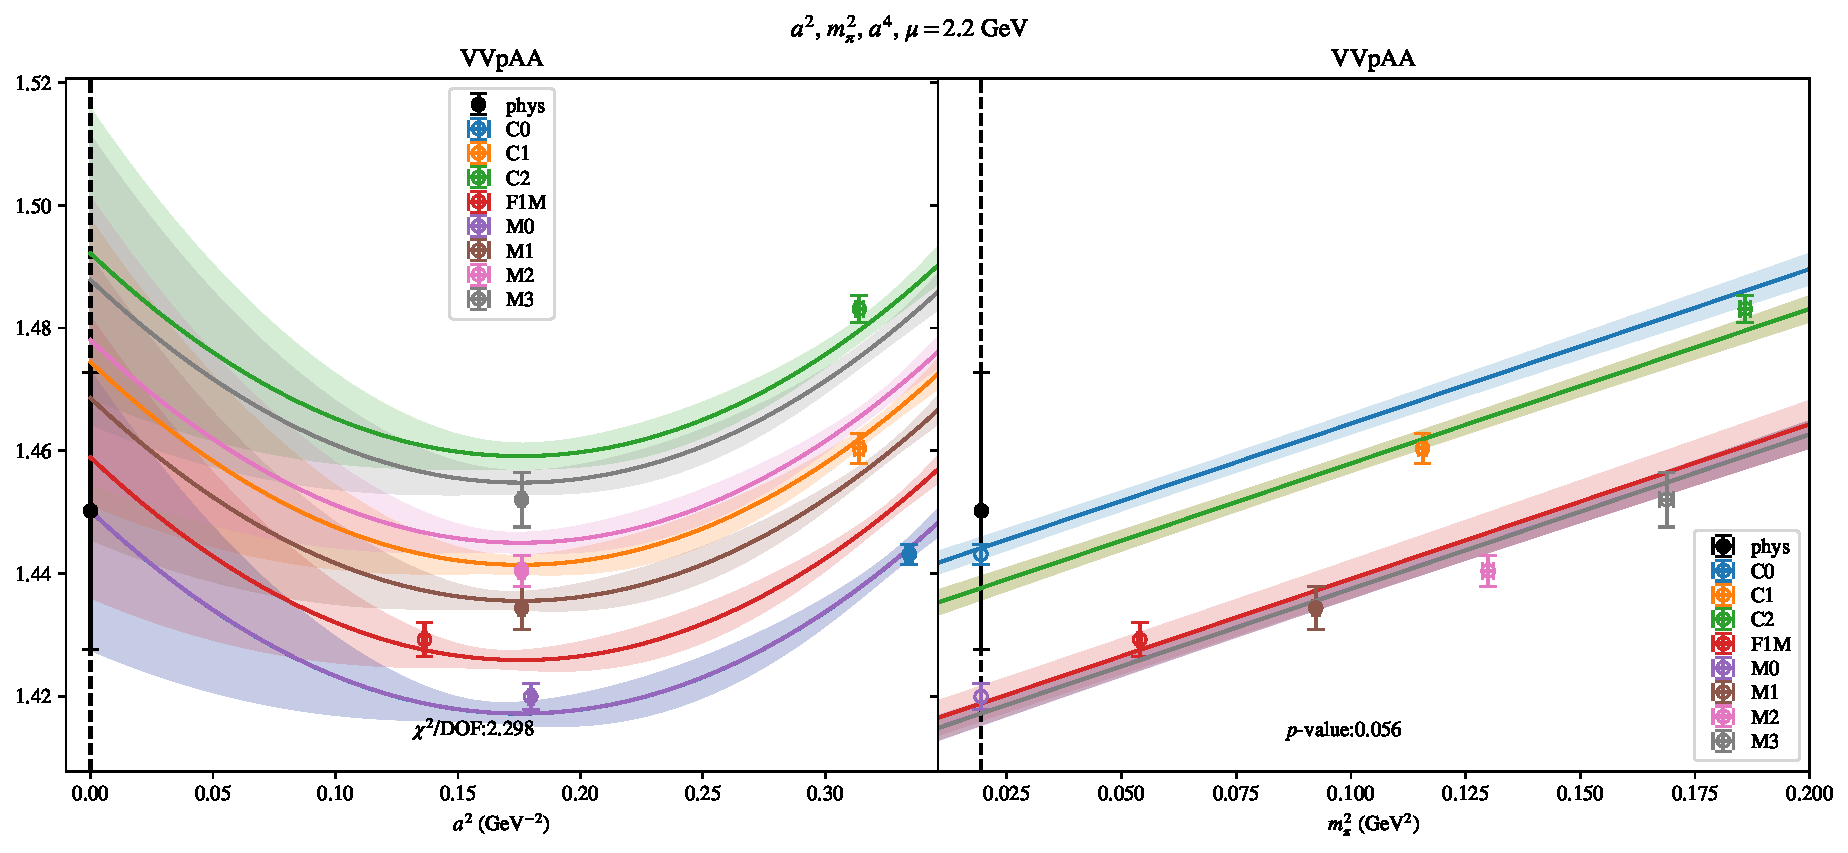
\includepdf[link, pages=-]{VVpAA/SUSY/bag_a2a4m2_22.pdf}
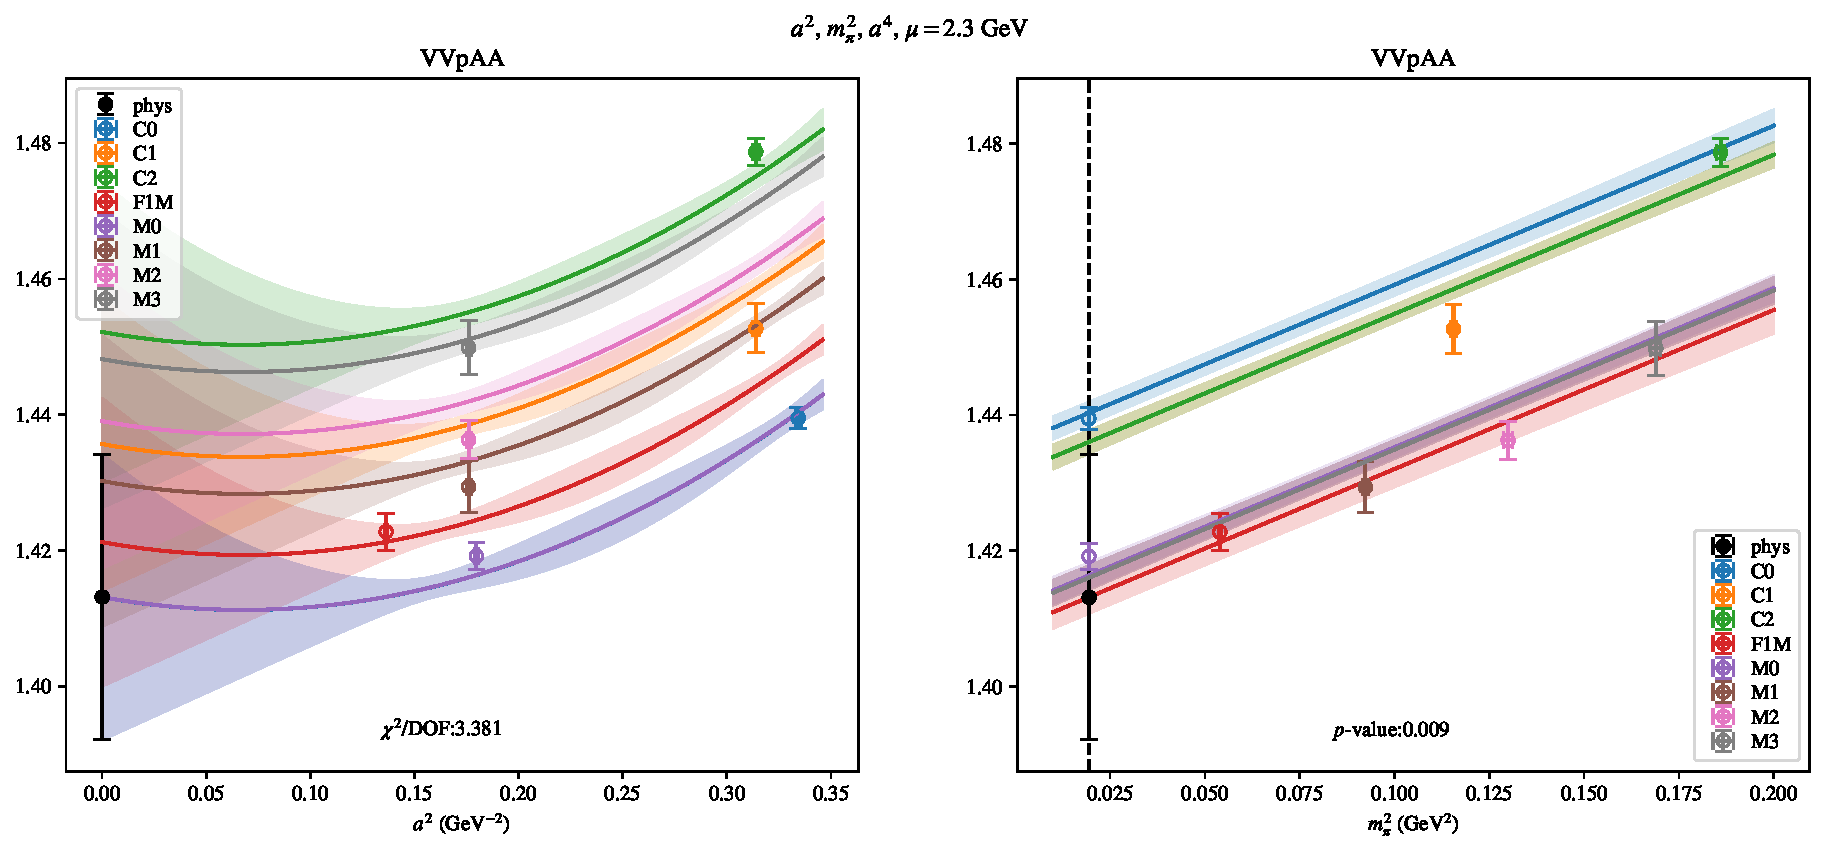
\includepdf[link, pages=-]{VVpAA/SUSY/bag_a2a4m2_23.pdf}
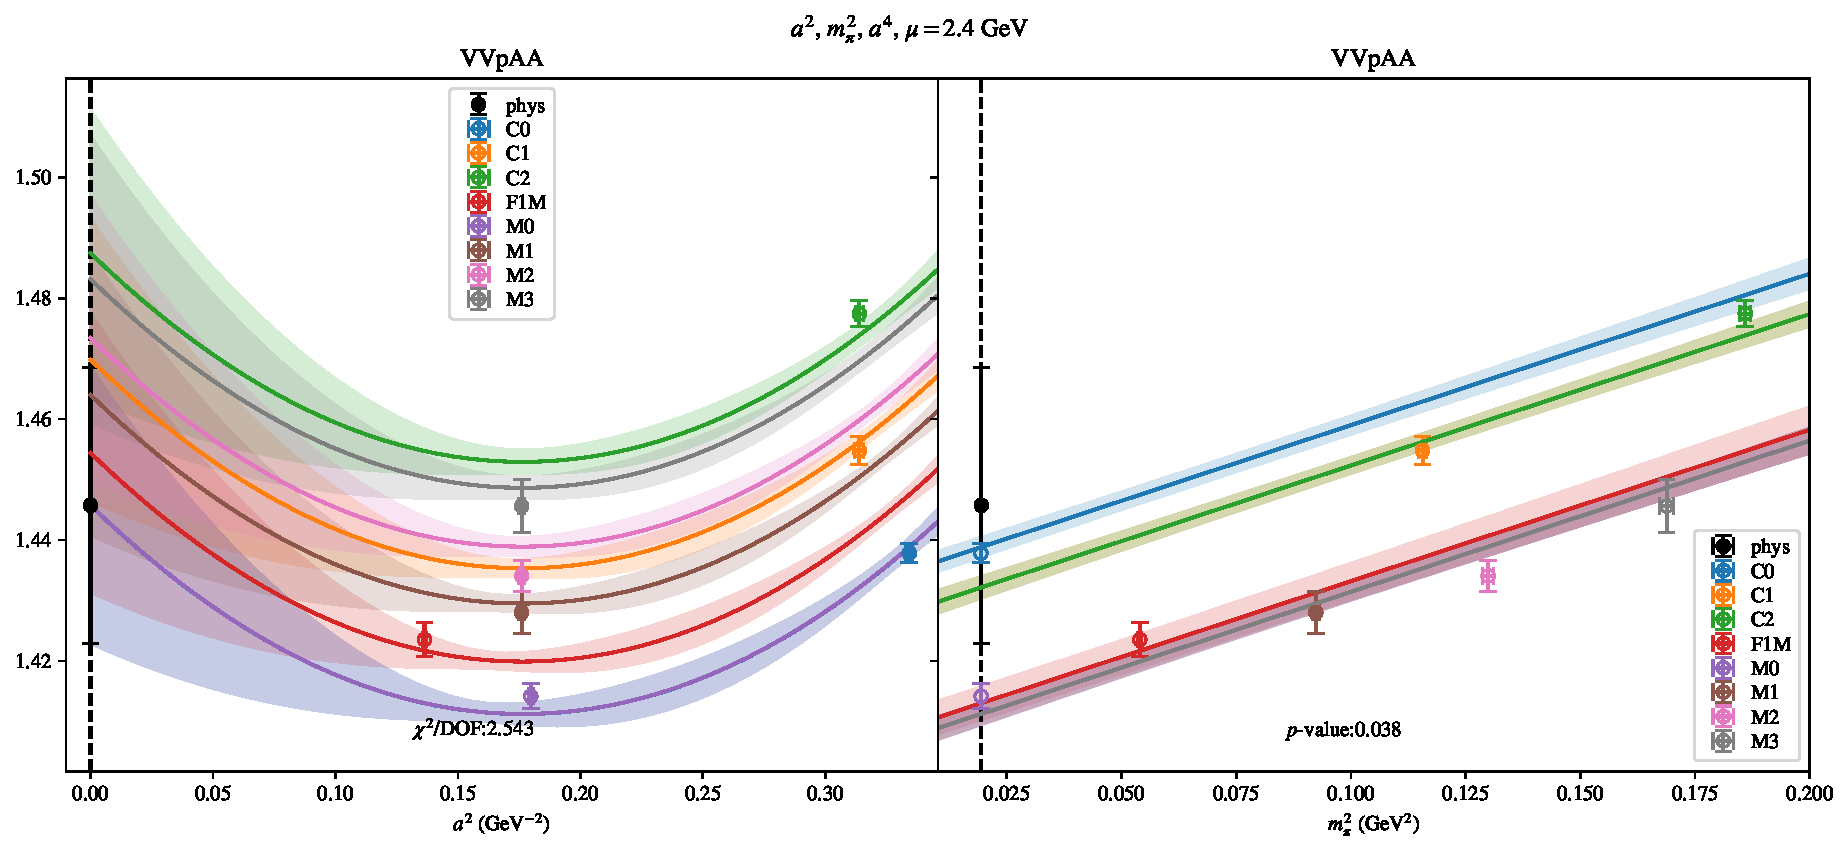
\includepdf[link, pages=-]{VVpAA/SUSY/bag_a2a4m2_24.pdf}
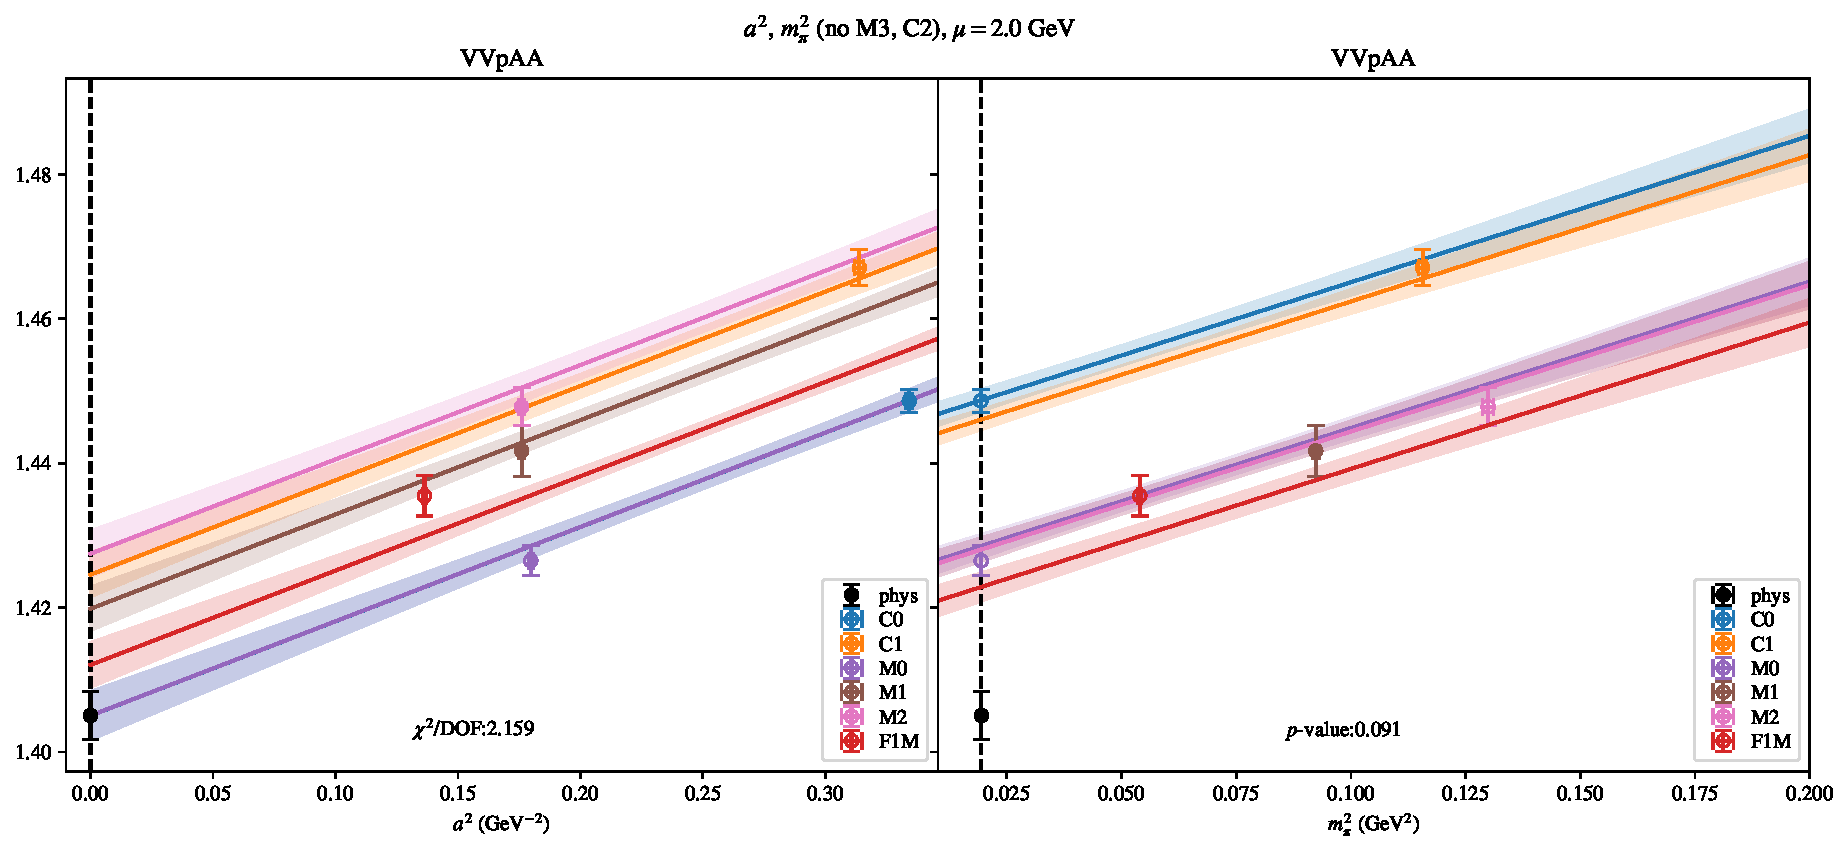
\includepdf[link, pages=-]{VVpAA/SUSY/bag_a2m2mcut_20.pdf}
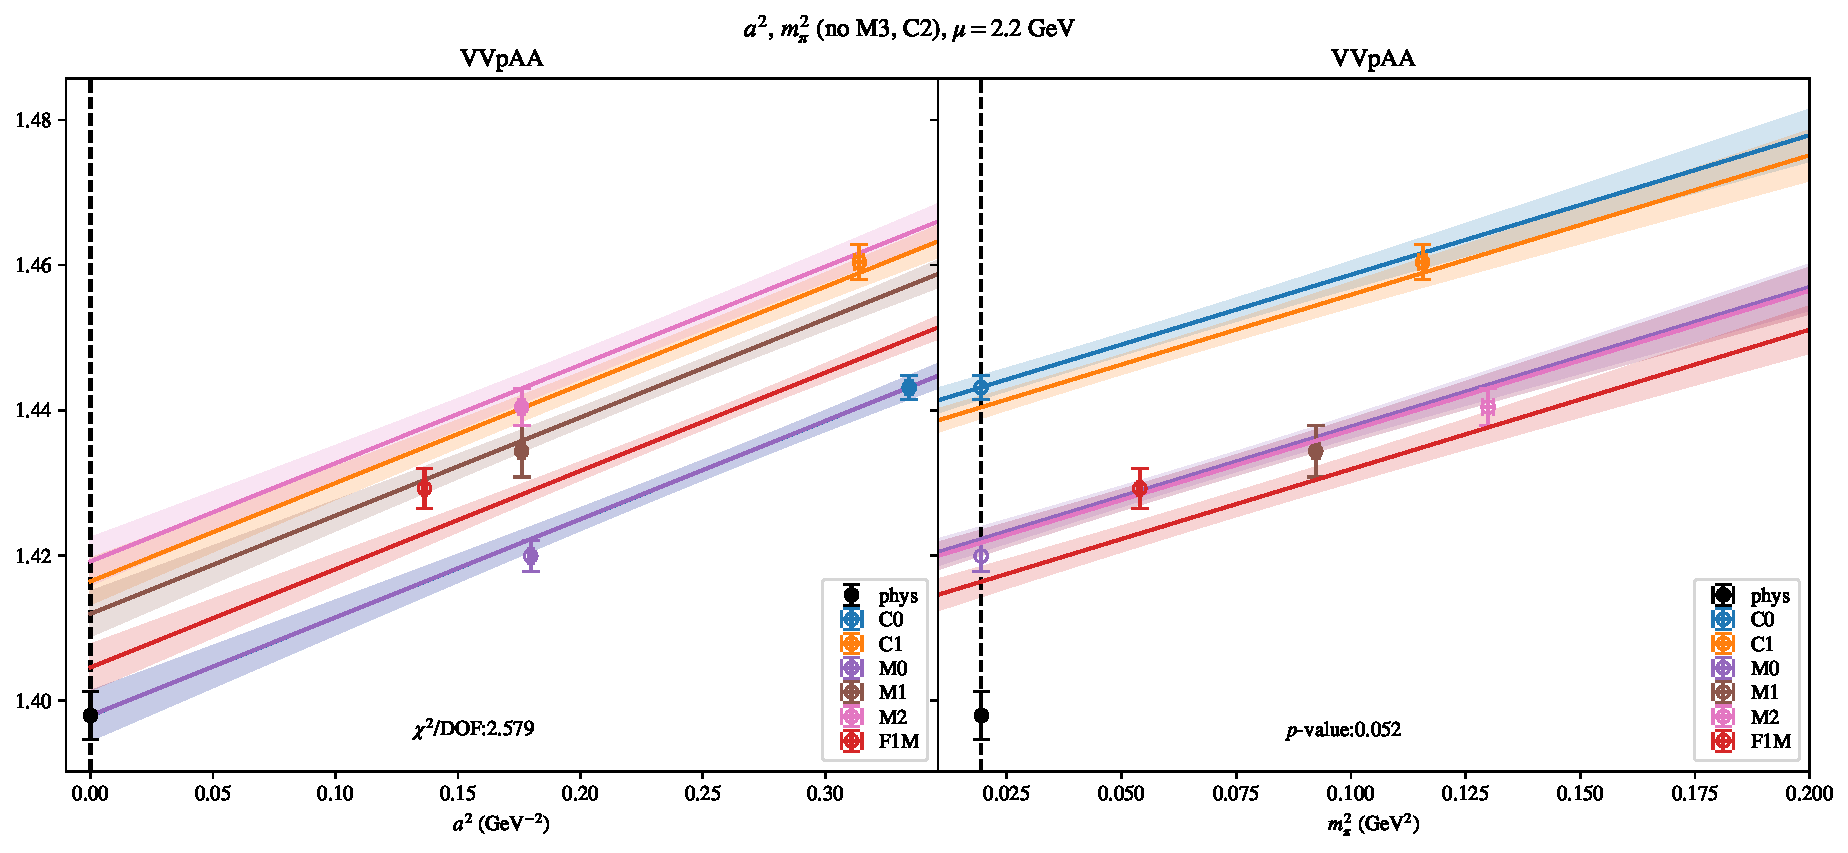
\includepdf[link, pages=-]{VVpAA/SUSY/bag_a2m2mcut_22.pdf}
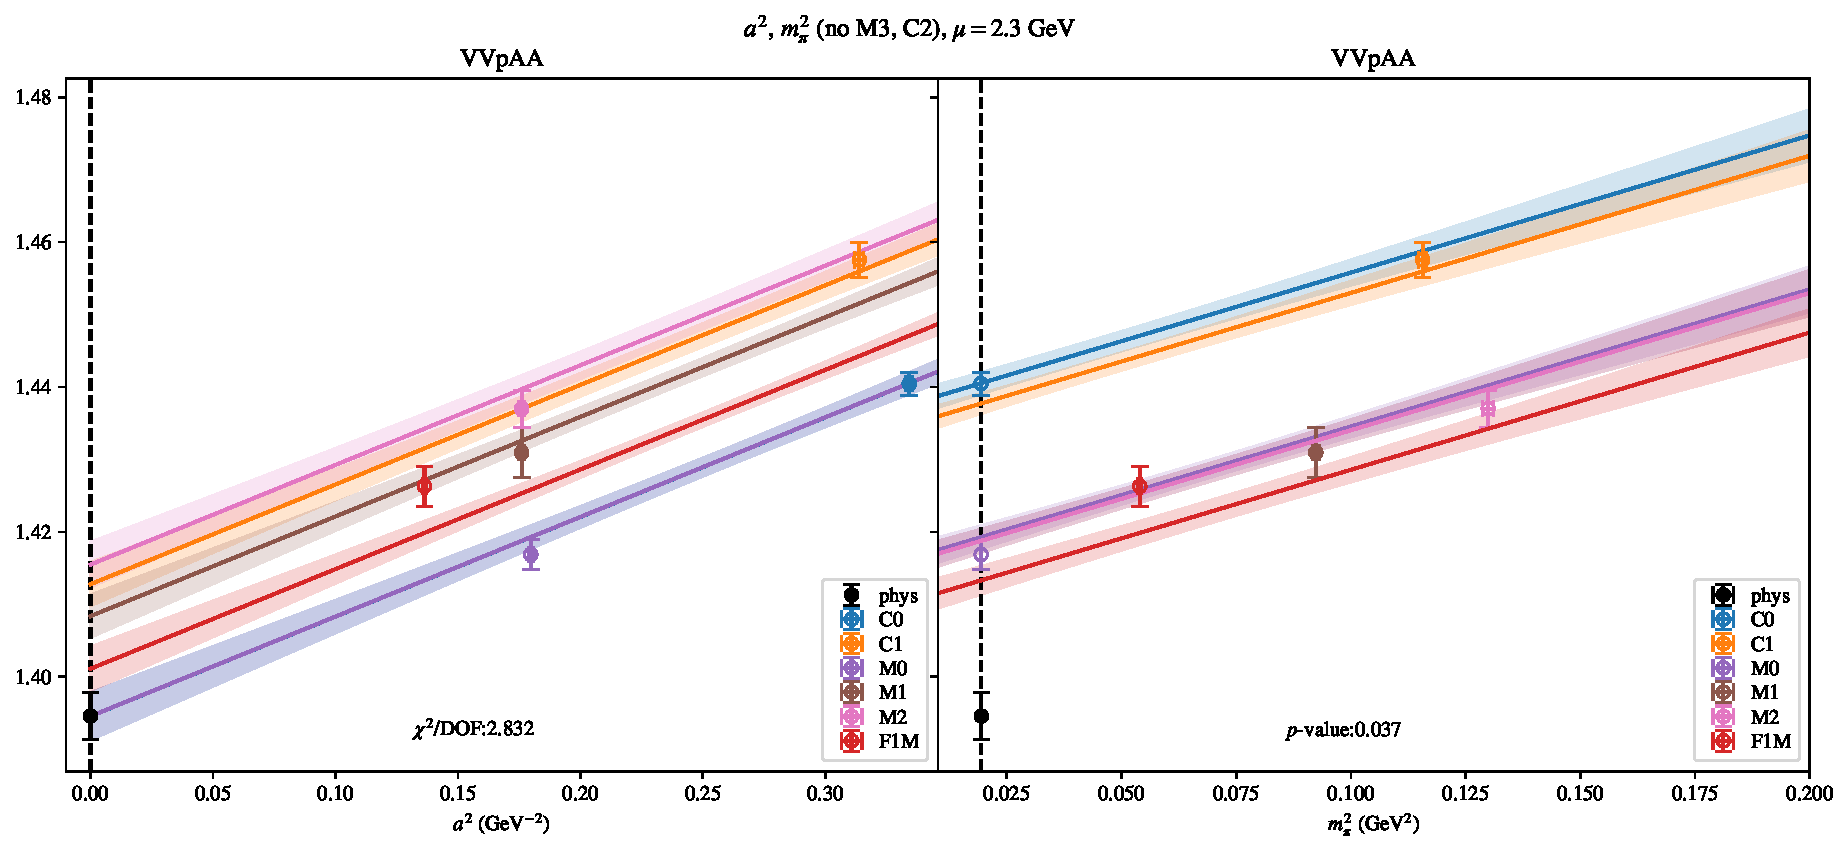
\includepdf[link, pages=-]{VVpAA/SUSY/bag_a2m2mcut_23.pdf}
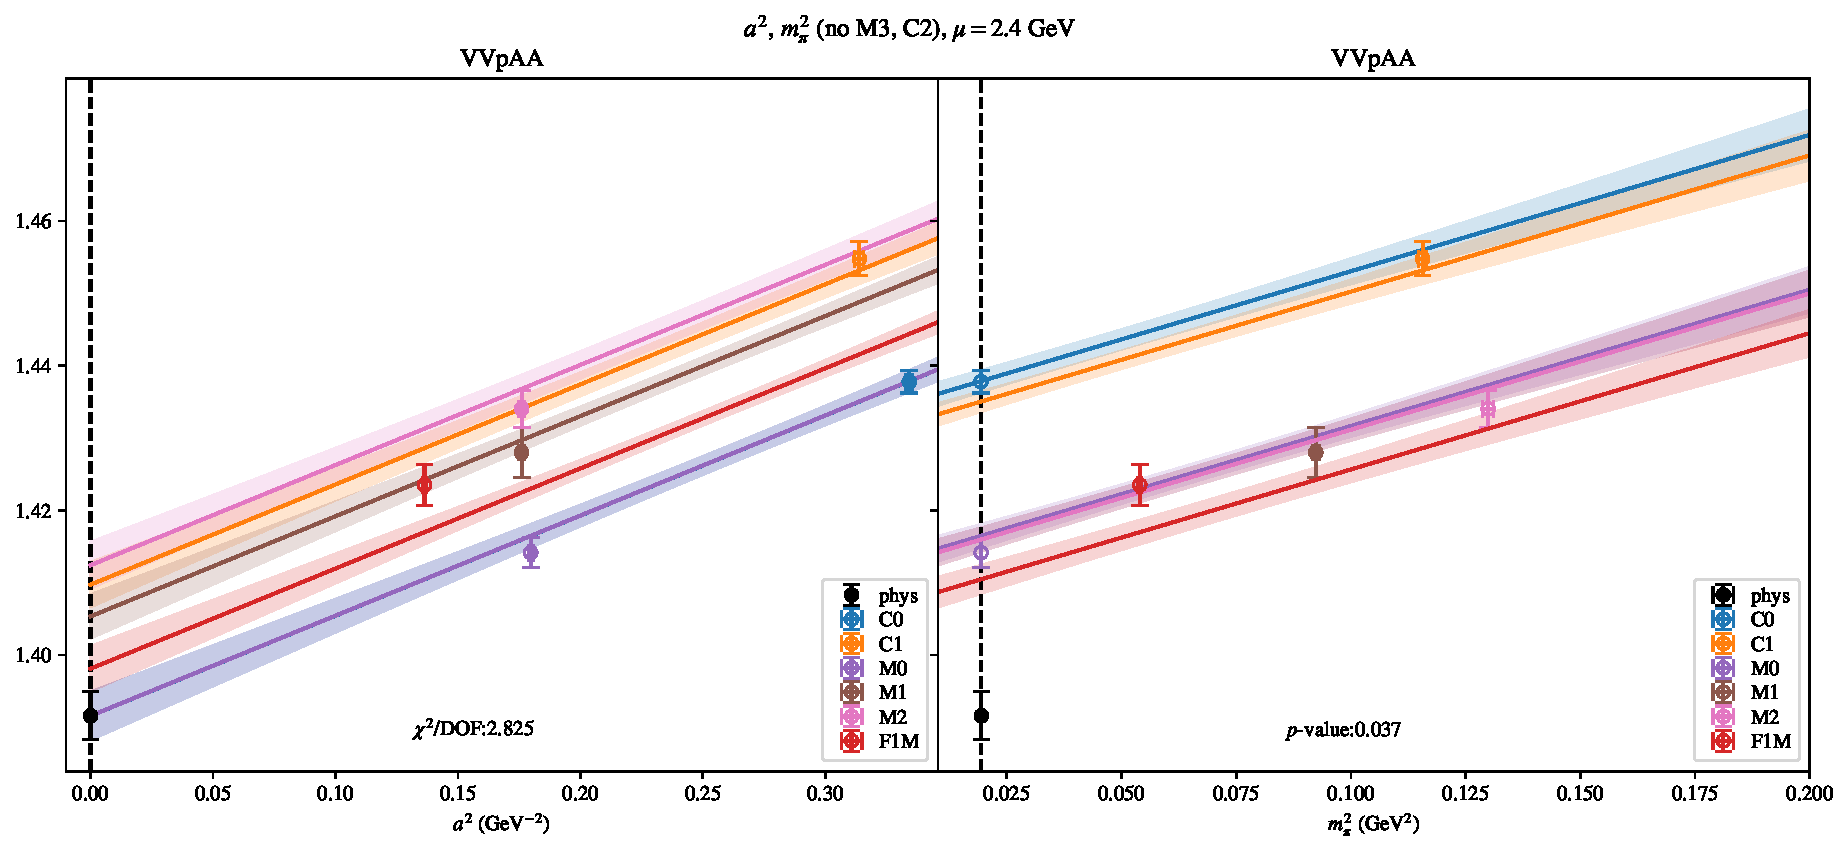
\includepdf[link, pages=-]{VVpAA/SUSY/bag_a2m2mcut_24.pdf}
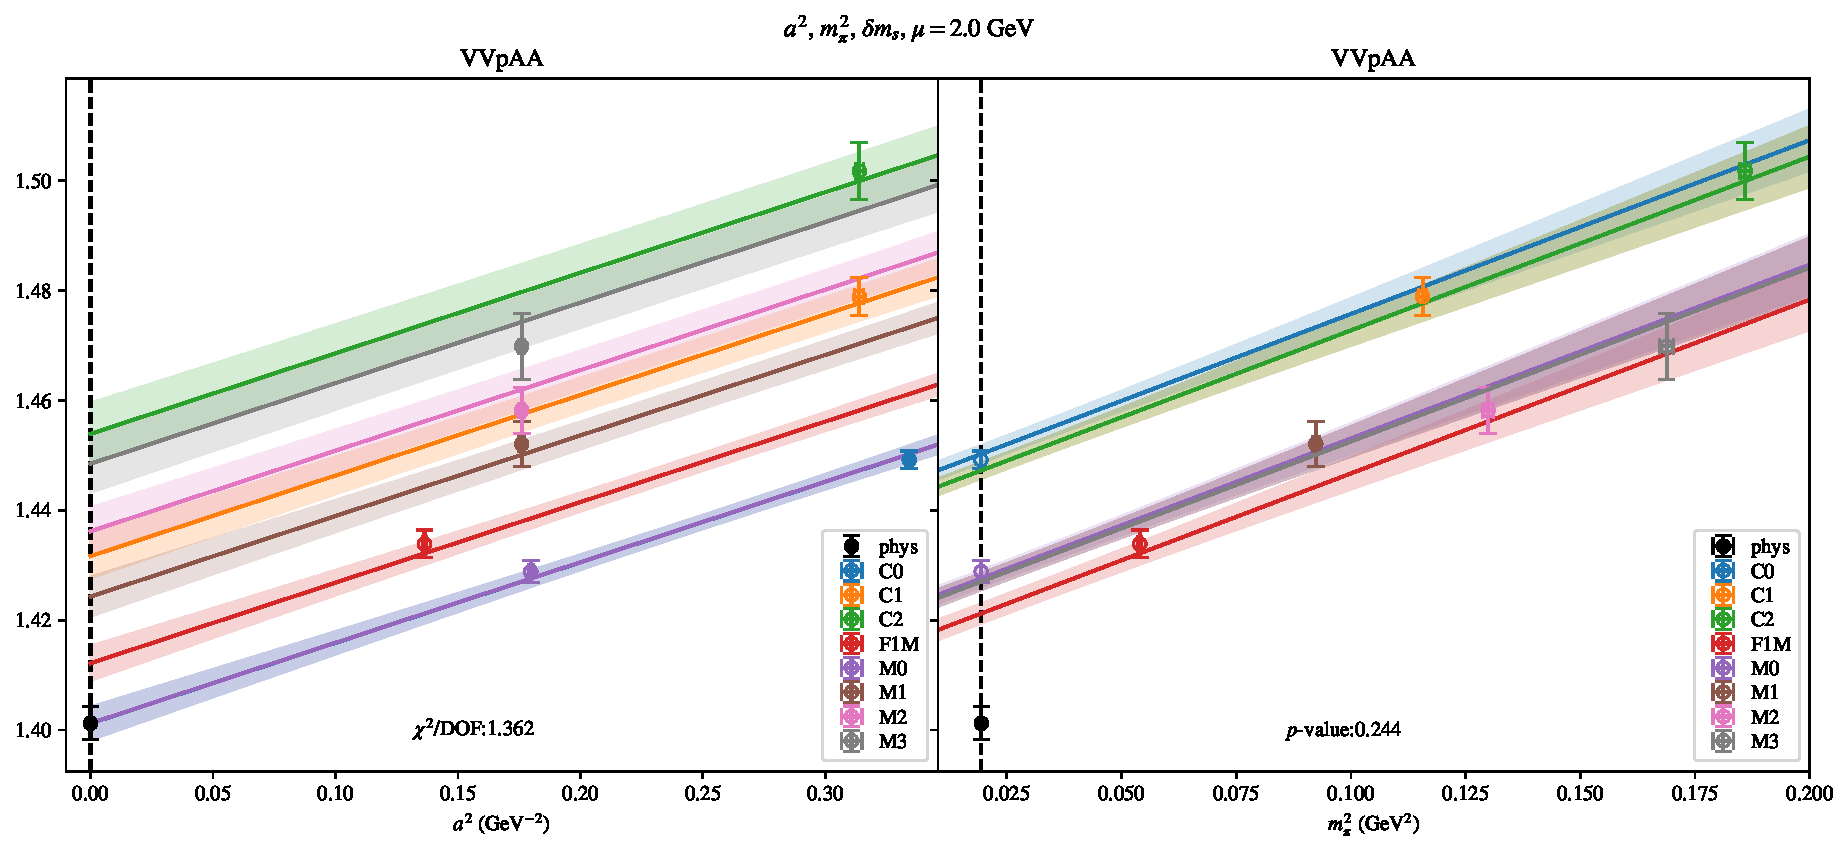
\includepdf[link, pages=-]{VVpAA/SUSY/bag_a2m2delm_20.pdf}
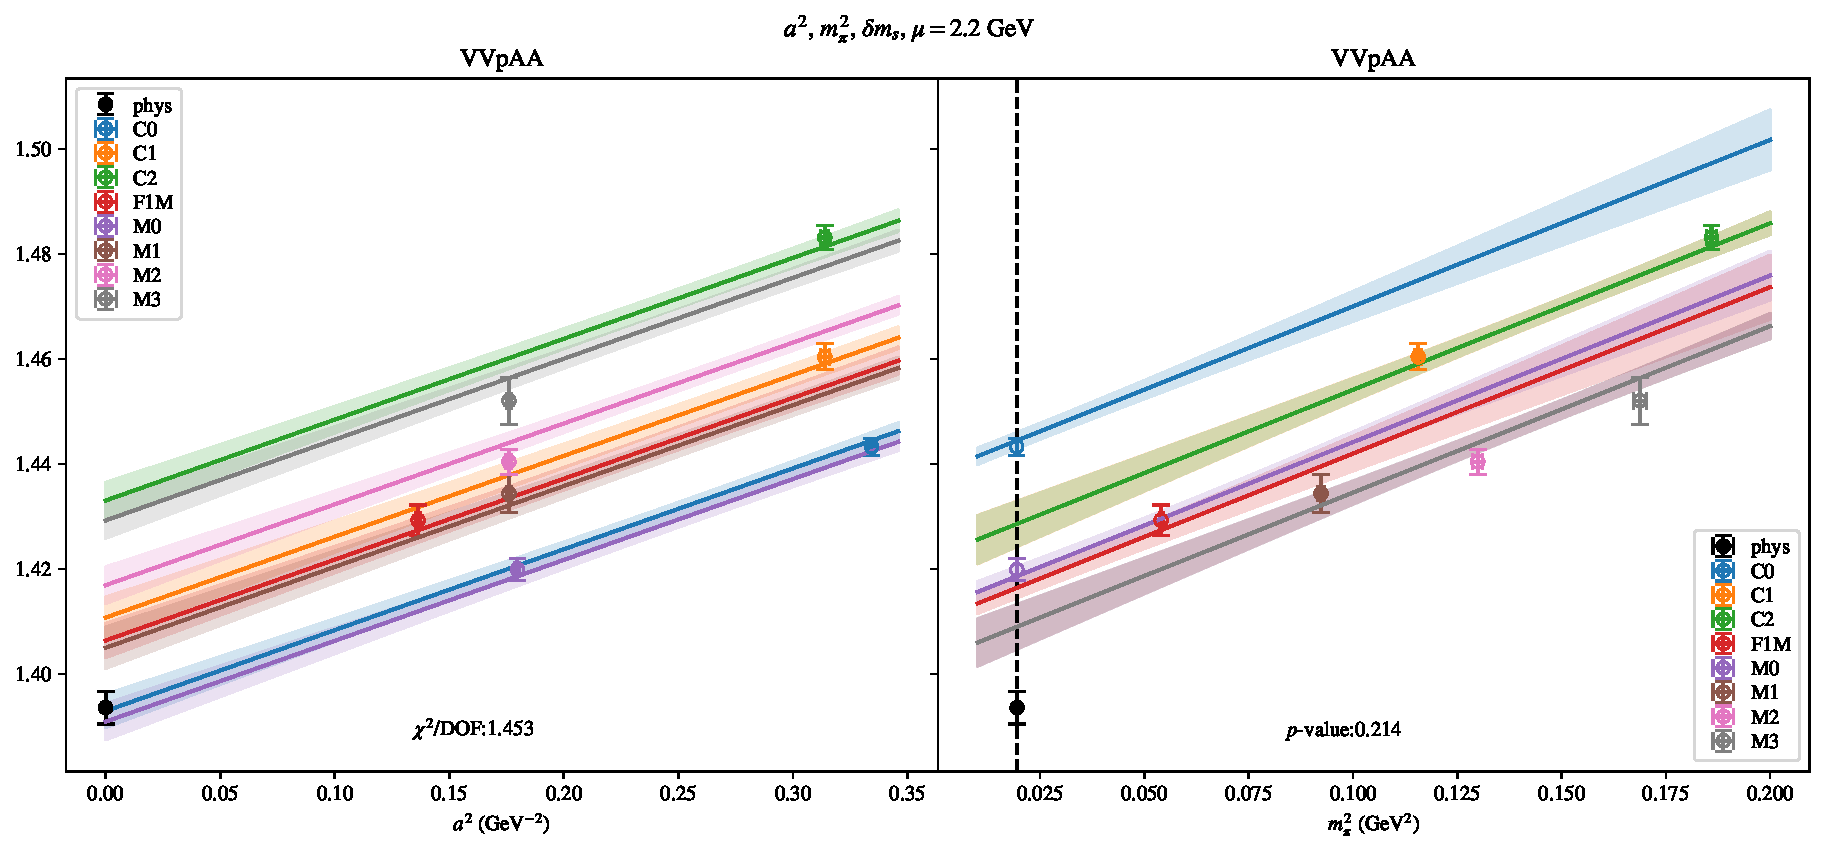
\includepdf[link, pages=-]{VVpAA/SUSY/bag_a2m2delm_22.pdf}
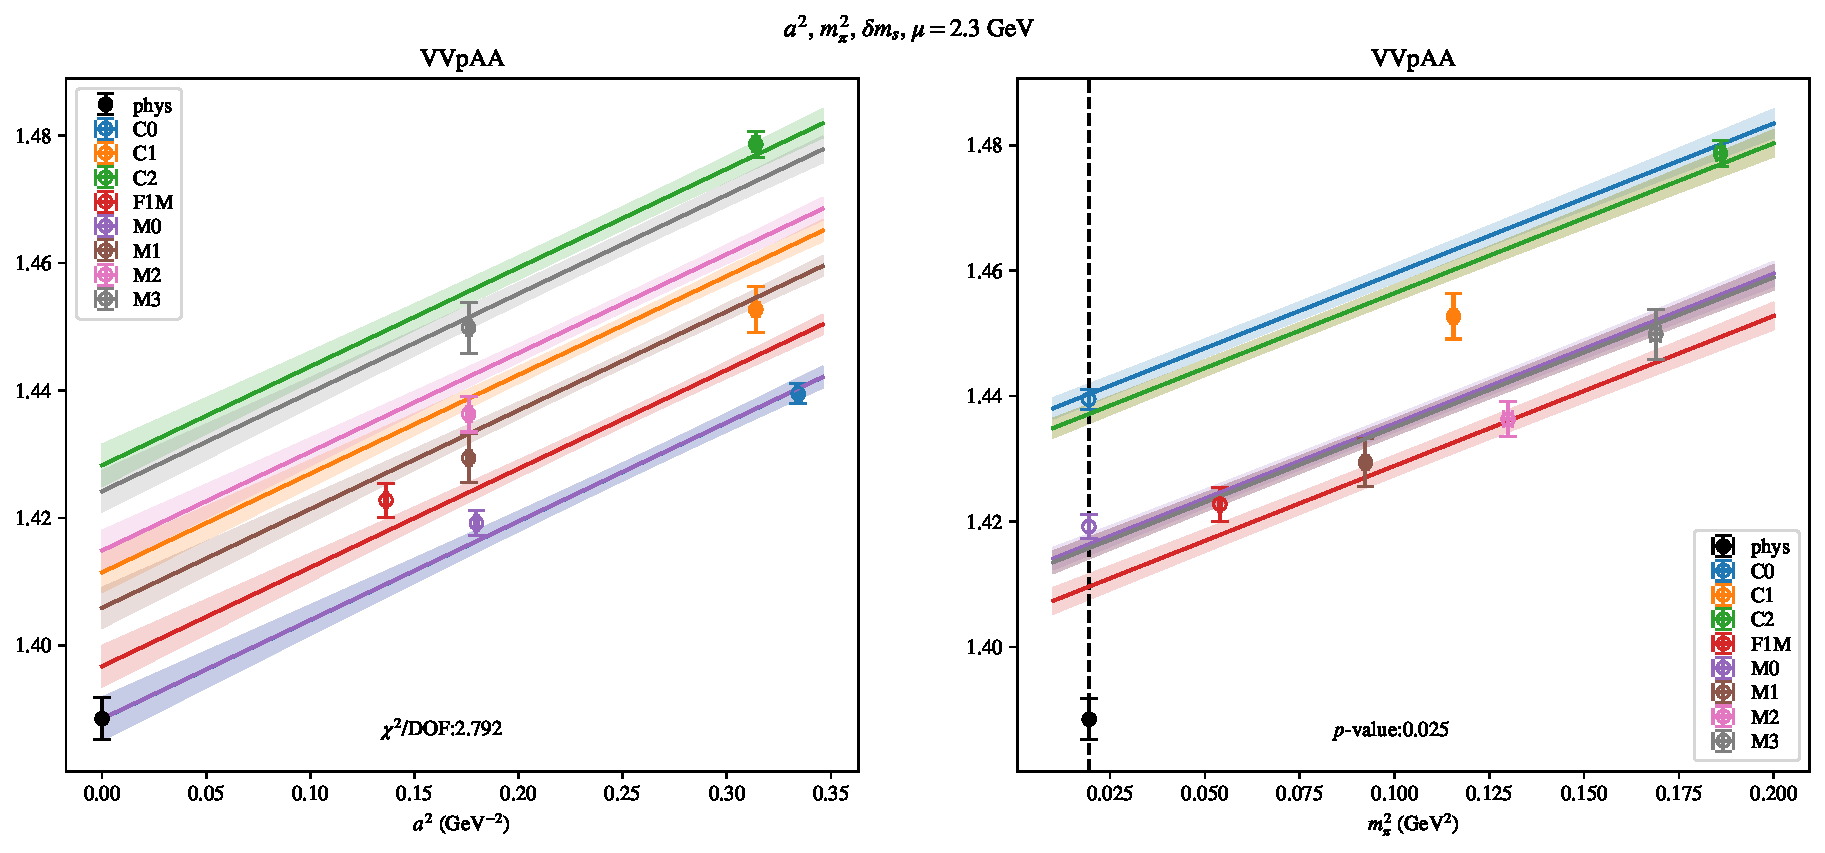
\includepdf[link, pages=-]{VVpAA/SUSY/bag_a2m2delm_23.pdf}
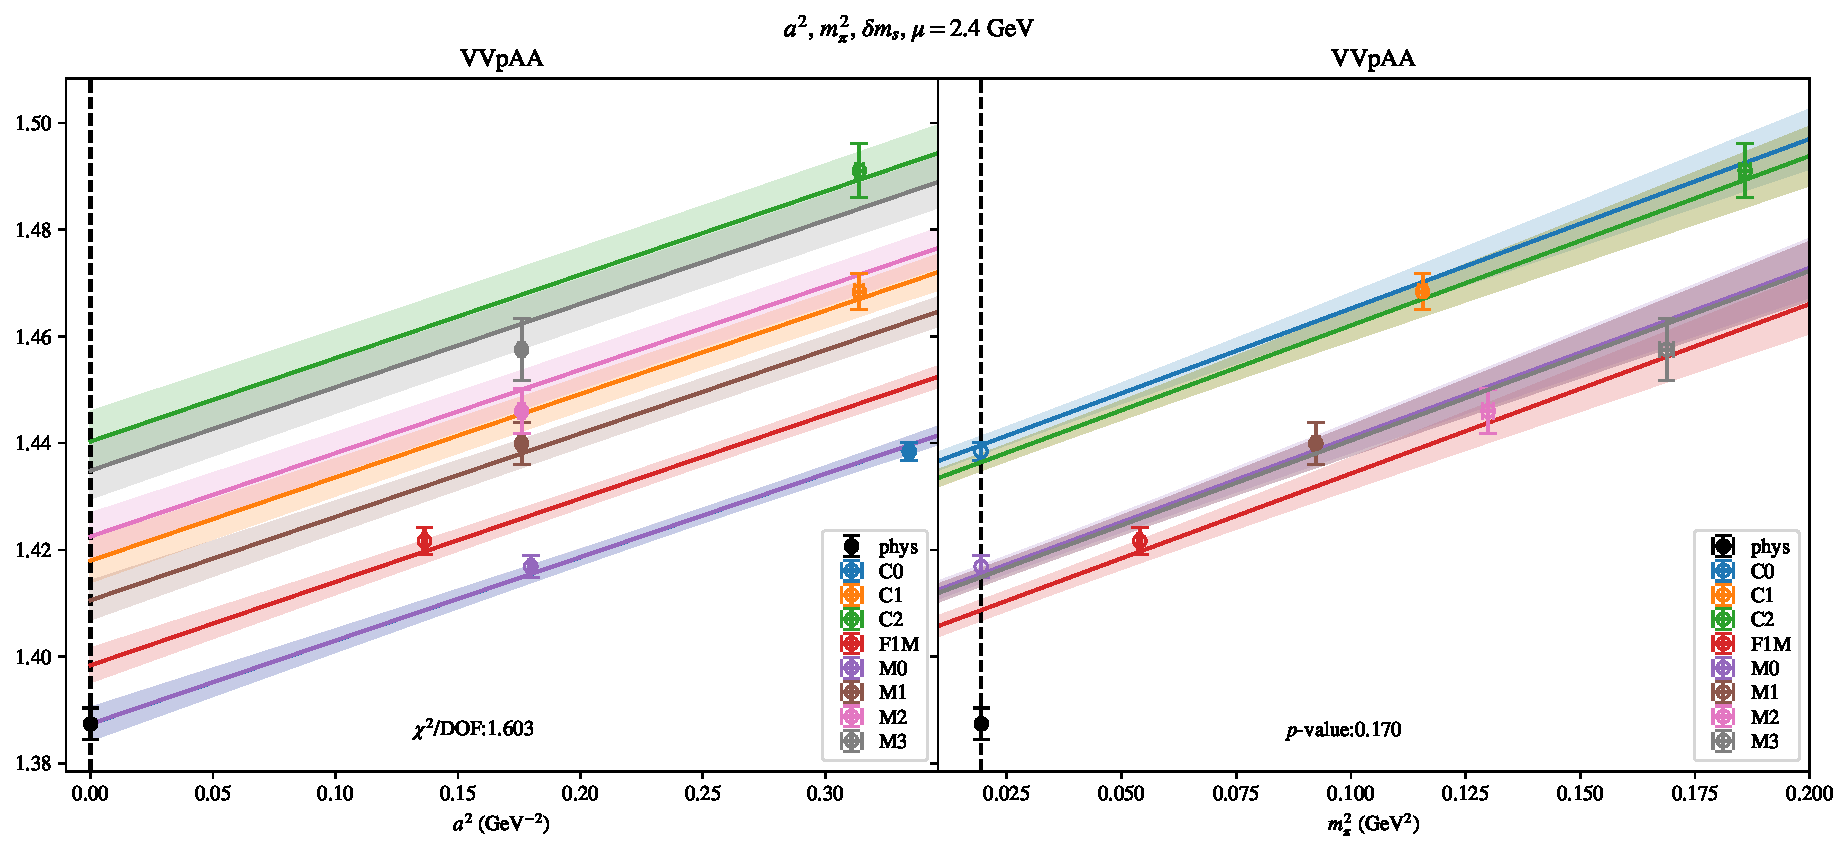
\includepdf[link, pages=-]{VVpAA/SUSY/bag_a2m2delm_24.pdf}
\clearpage
\section{$\mathcal{B}_2$}
\begin{table}[h!]
\begin{center}
\begin{tabular}{|c|c|c|c|c|c|}
\hline
$\mu$ (GeV) & $a^2$, $m_\pi^2$& $a^2$, $m_\pi^2$ (no C)& $a^2$, $m_\pi^2$, $a^4$& $a^2$, $m_\pi^2$ (no M3, C2)& $a^2$, $m_\pi^2$, $\delta m_s$\\
\hline
2.0& \hyperlink{VVmAA/SUSY/bag_a2m2_20.pdf.1}{\textbf{-0.9273(27)}: 1.086 (0.366)} & \hyperlink{VVmAA/SUSY/bag_a2m2noC_20.pdf.1}{\textbf{-0.943(10)}: 0.73 (0.482)} & \hyperlink{VVmAA/SUSY/bag_a2a4m2_20.pdf.1}{\textbf{-0.951(18)}: 0.878 (0.476)} & \hyperlink{VVmAA/SUSY/bag_a2m2mcut_20.pdf.1}{\textbf{-0.9263(28)}: 0.781 (0.504)} & \hyperlink{VVmAA/SUSY/bag_a2m2delm_20.pdf.1}{\textbf{-0.9273(27)}: 1.295 (0.269)}\\
2.2& \hyperlink{VVmAA/SUSY/bag_a2m2_22.pdf.1}{\textbf{-0.9080(21)}: 2.142 (0.057)} & \hyperlink{VVmAA/SUSY/bag_a2m2noC_22.pdf.1}{\textbf{-0.9283(87)}: 0.738 (0.478)} & \hyperlink{VVmAA/SUSY/bag_a2a4m2_22.pdf.1}{\textbf{-0.933(15)}: 1.85 (0.116)} & \hyperlink{VVmAA/SUSY/bag_a2m2mcut_22.pdf.1}{\textbf{-0.9074(23)}: 2.062 (0.103)} & \hyperlink{VVmAA/SUSY/bag_a2m2delm_22.pdf.1}{\textbf{-0.9080(21)}: 2.551 (0.037)}\\
2.3& \hyperlink{VVmAA/SUSY/bag_a2m2_23.pdf.1}{\textbf{-0.8990(20)}: 3.138 (0.008)} & \hyperlink{VVmAA/SUSY/bag_a2m2noC_23.pdf.1}{\textbf{-0.9210(80)}: 1.037 (0.355)} & \hyperlink{VVmAA/SUSY/bag_a2a4m2_23.pdf.1}{\textbf{-0.925(14)}: 2.939 (0.019)} & \hyperlink{VVmAA/SUSY/bag_a2m2mcut_23.pdf.1}{\textbf{-0.8984(22)}: 3.297 (0.02)} & \hyperlink{VVmAA/SUSY/bag_a2m2delm_23.pdf.1}{\textbf{-0.8989(20)}: 3.796 (0.004)}\\
2.4& \hyperlink{VVmAA/SUSY/bag_a2m2_24.pdf.1}{\textbf{-0.8909(20)}: 3.842 (0.002)} & \hyperlink{VVmAA/SUSY/bag_a2m2noC_24.pdf.1}{\textbf{-0.9139(78)}: 1.326 (0.265)} & \hyperlink{VVmAA/SUSY/bag_a2a4m2_24.pdf.1}{\textbf{-0.917(14)}: 3.736 (0.005)} & \hyperlink{VVmAA/SUSY/bag_a2m2mcut_24.pdf.1}{\textbf{-0.8905(21)}: 4.224 (0.005)} & \hyperlink{VVmAA/SUSY/bag_a2m2delm_24.pdf.1}{\textbf{-0.8909(19)}: 4.697 (0.001)}\\
\hline
\end{tabular}
\caption{Physical point value from chiral and continuum extrapolation at renormalisation scale $\mu$. Entries are \textbf{value(error)}: $\chi^2/\text{DOF}$ ($p$-value).}
\end{center}
\end{table}
\begin{table}[h!]
\begin{center}
\begin{tabular}{|c c|c|c|c|c|c|}
\hline
$\mu$ (GeV) &  & $a^2$, $m_\pi^2$& $a^2$, $m_\pi^2$ (no C)& $a^2$, $m_\pi^2$, $a^4$& $a^2$, $m_\pi^2$ (no M3, C2)& $a^2$, $m_\pi^2$, $\delta m_s$\\
\hline
\multirow{3}{0.5in}{2.0} & $\alpha$ & -0.349(11)& -0.256(62)& -0.13(16)& -0.352(11)& -0.350(11)\\
 & $\beta$ & -0.00699(27)& -0.00694(49)& -0.00703(27)& -0.00765(47)& -0.00719(47)\\
 & $\gamma$ &  &  & -0.44(33)&  & 0.009(17)\\
\hline
\multirow{3}{0.5in}{2.2} & $\alpha$ & -0.3785(85)& -0.260(50)& -0.15(14)& -0.3801(90)& -0.3794(85)\\
 & $\beta$ & -0.00678(21)& -0.00642(40)& -0.00686(22)& -0.00731(36)& -0.00702(38)\\
 & $\gamma$ &  &  & -0.47(28)&  & 0.010(13)\\
\hline
\multirow{3}{0.5in}{2.3} & $\alpha$ & -0.3951(82)& -0.267(46)& -0.16(13)& -0.3962(86)& -0.3959(82)\\
 & $\beta$ & -0.00687(20)& -0.00642(34)& -0.00696(20)& -0.00737(34)& -0.00709(36)\\
 & $\gamma$ &  &  & -0.48(27)&  & 0.009(12)\\
\hline
\multirow{3}{0.5in}{2.4} & $\alpha$ & -0.4103(80)& -0.278(45)& -0.17(13)& -0.4107(84)& -0.4110(80)\\
 & $\beta$ & -0.00683(18)& -0.00636(29)& -0.00692(18)& -0.00729(29)& -0.00702(34)\\
 & $\gamma$ &  &  & -0.49(27)&  & 0.008(12)\\
\hline
\end{tabular}
\caption{Fit values of coefficients in $Q = Q_{phys} + \mathbf{\alpha} a^2 + \mathbf{\beta}\left(\frac{m_\pi^2}{f_\pi^2}-\frac{m_{\pi,PDG}^2}{f_\pi^2}\right) + \gamma(\ldots)$}
\end{center}
\end{table}
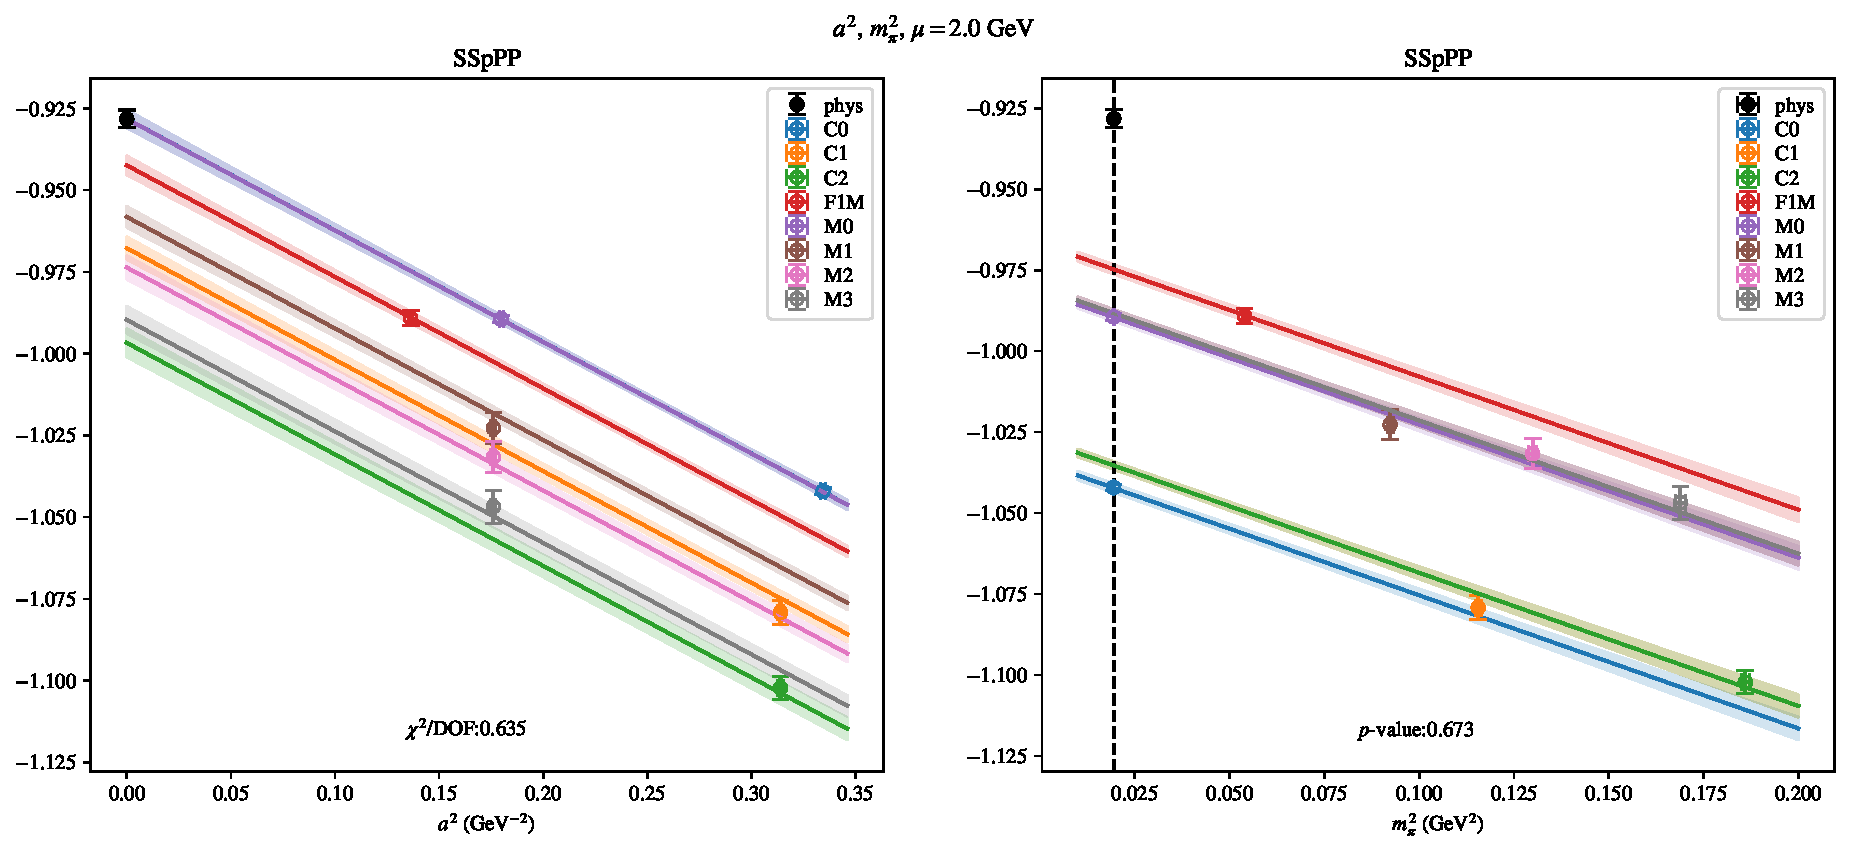
\includepdf[link, pages=-]{VVmAA/SUSY/bag_a2m2_20.pdf}
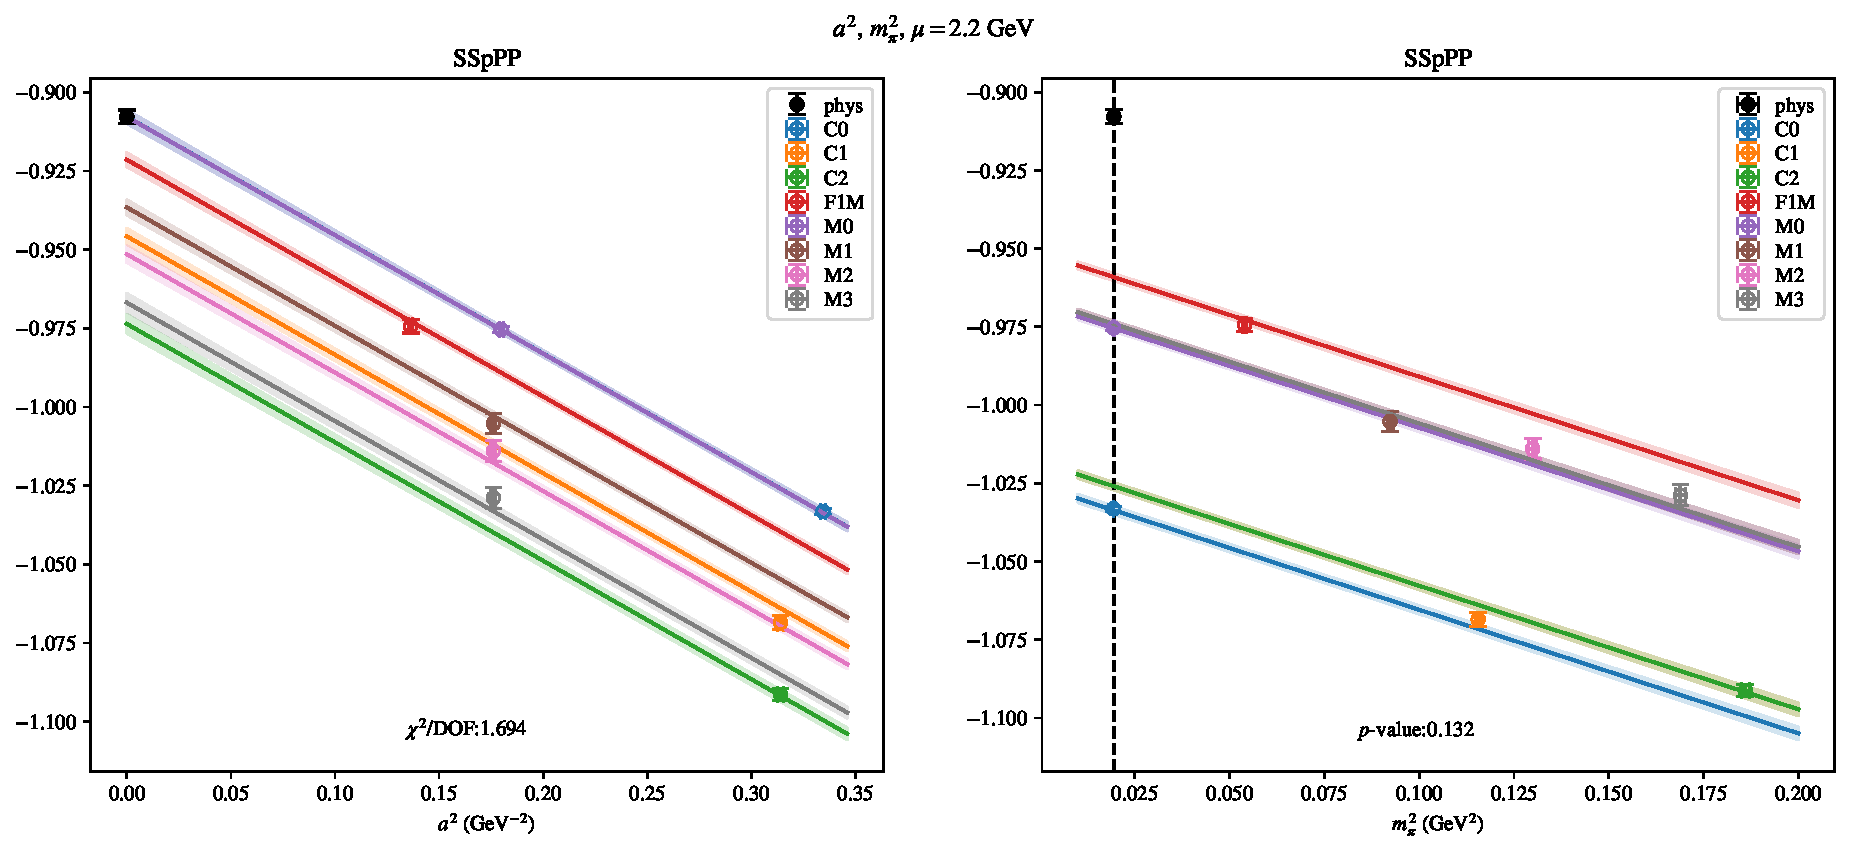
\includepdf[link, pages=-]{VVmAA/SUSY/bag_a2m2_22.pdf}
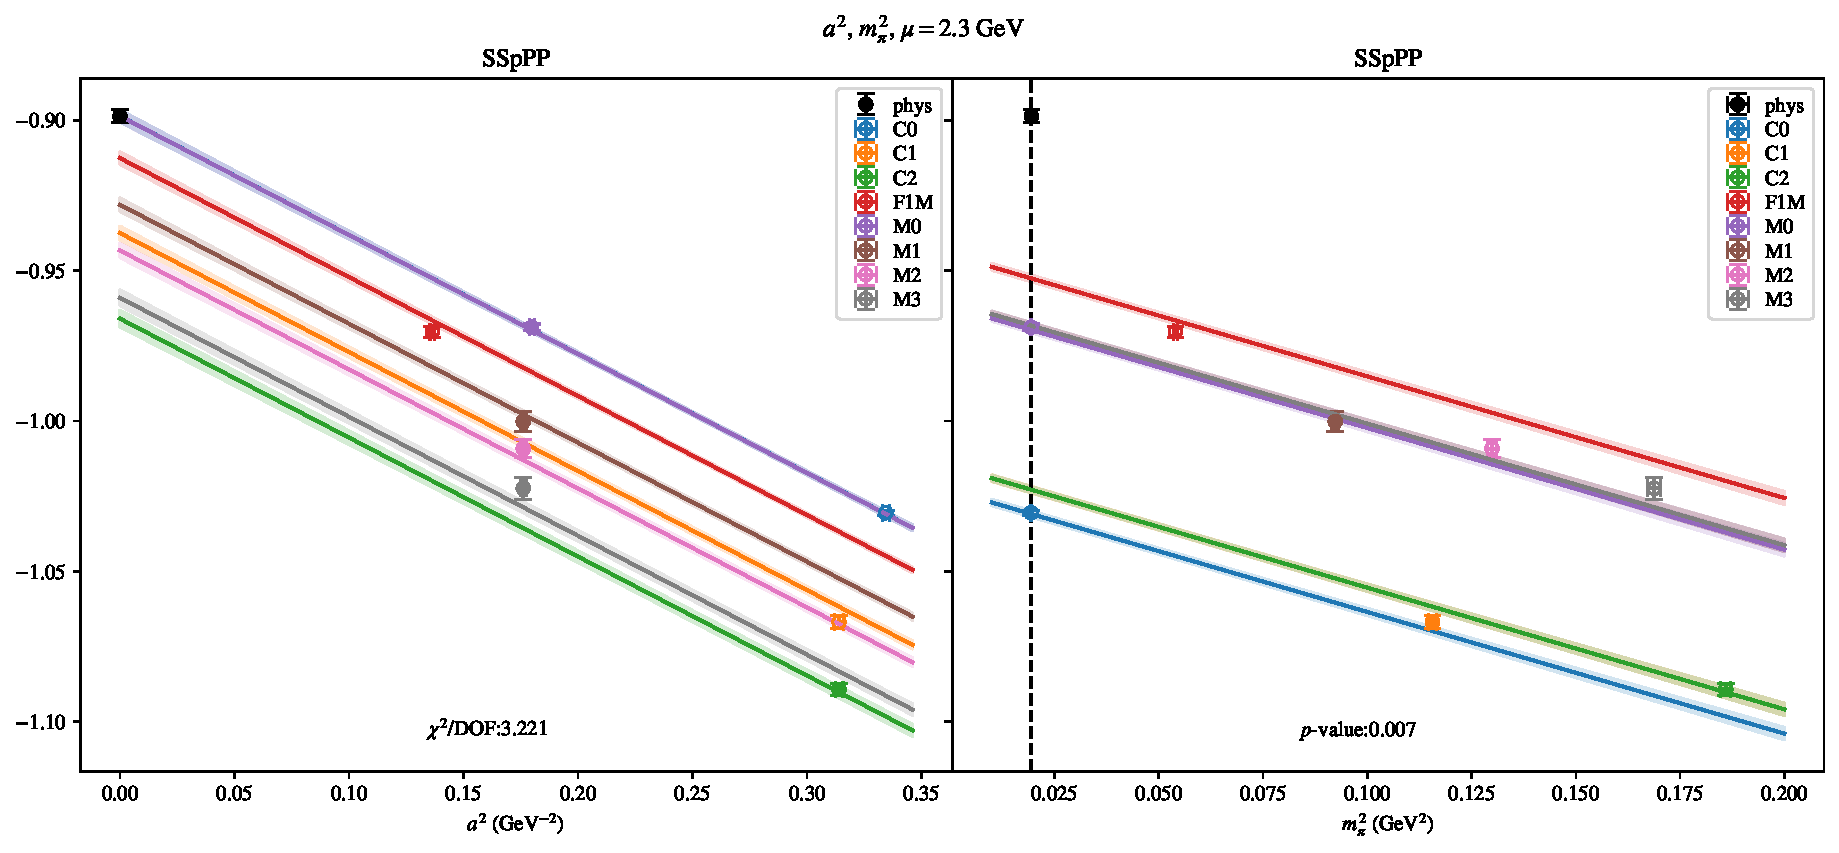
\includepdf[link, pages=-]{VVmAA/SUSY/bag_a2m2_23.pdf}
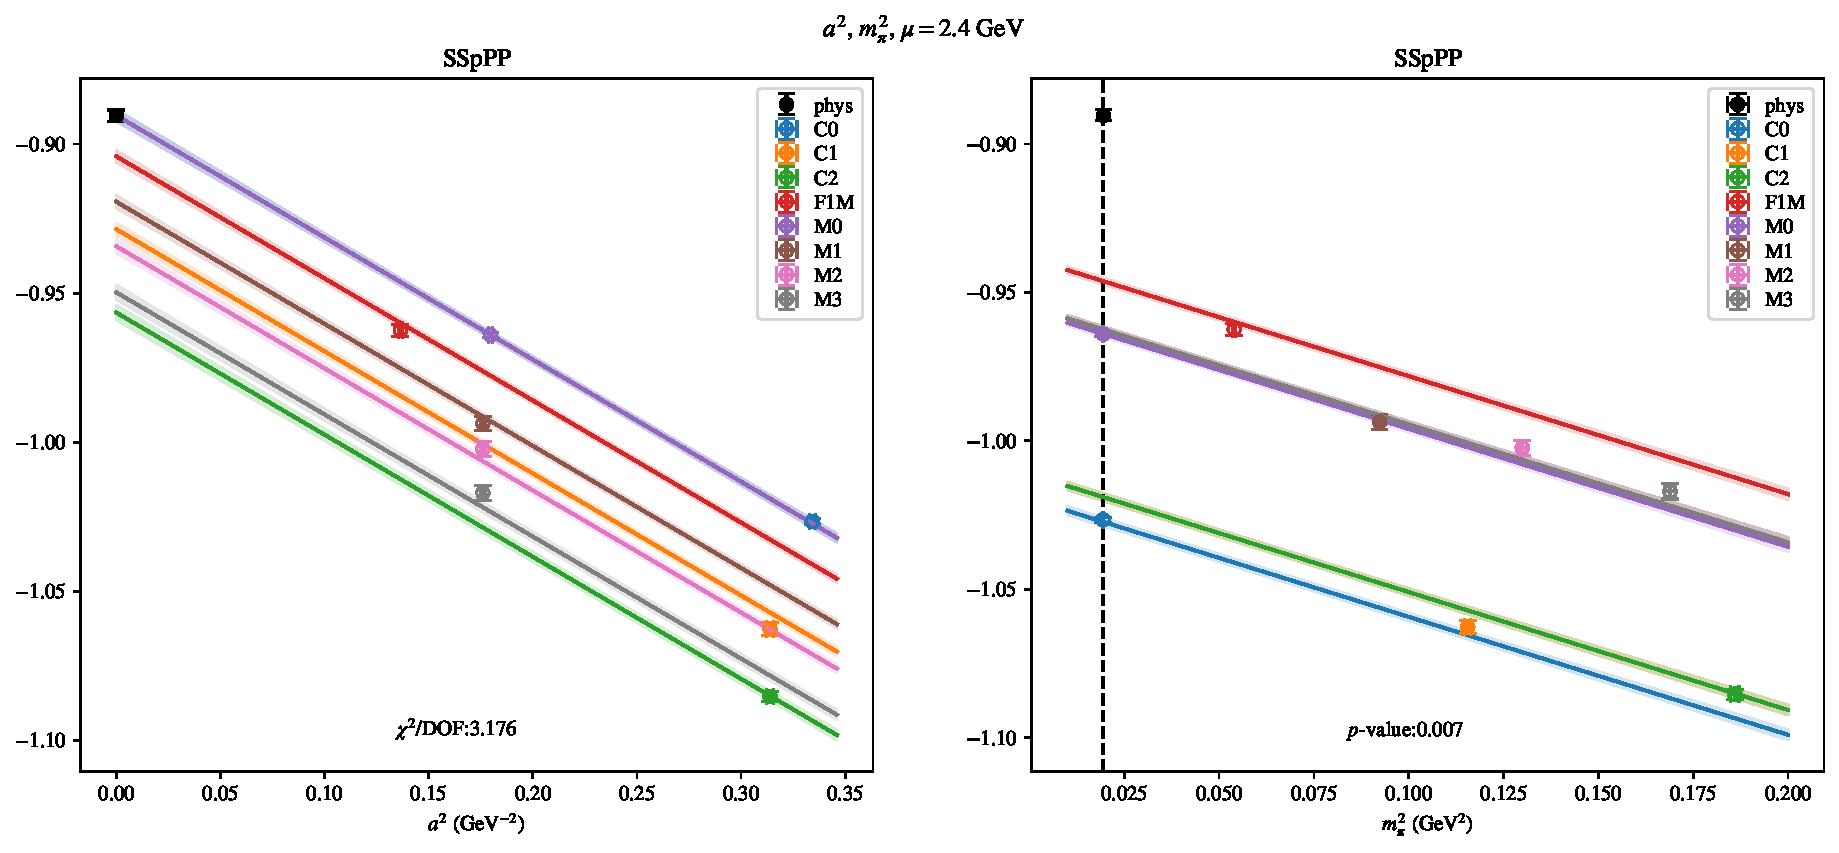
\includepdf[link, pages=-]{VVmAA/SUSY/bag_a2m2_24.pdf}
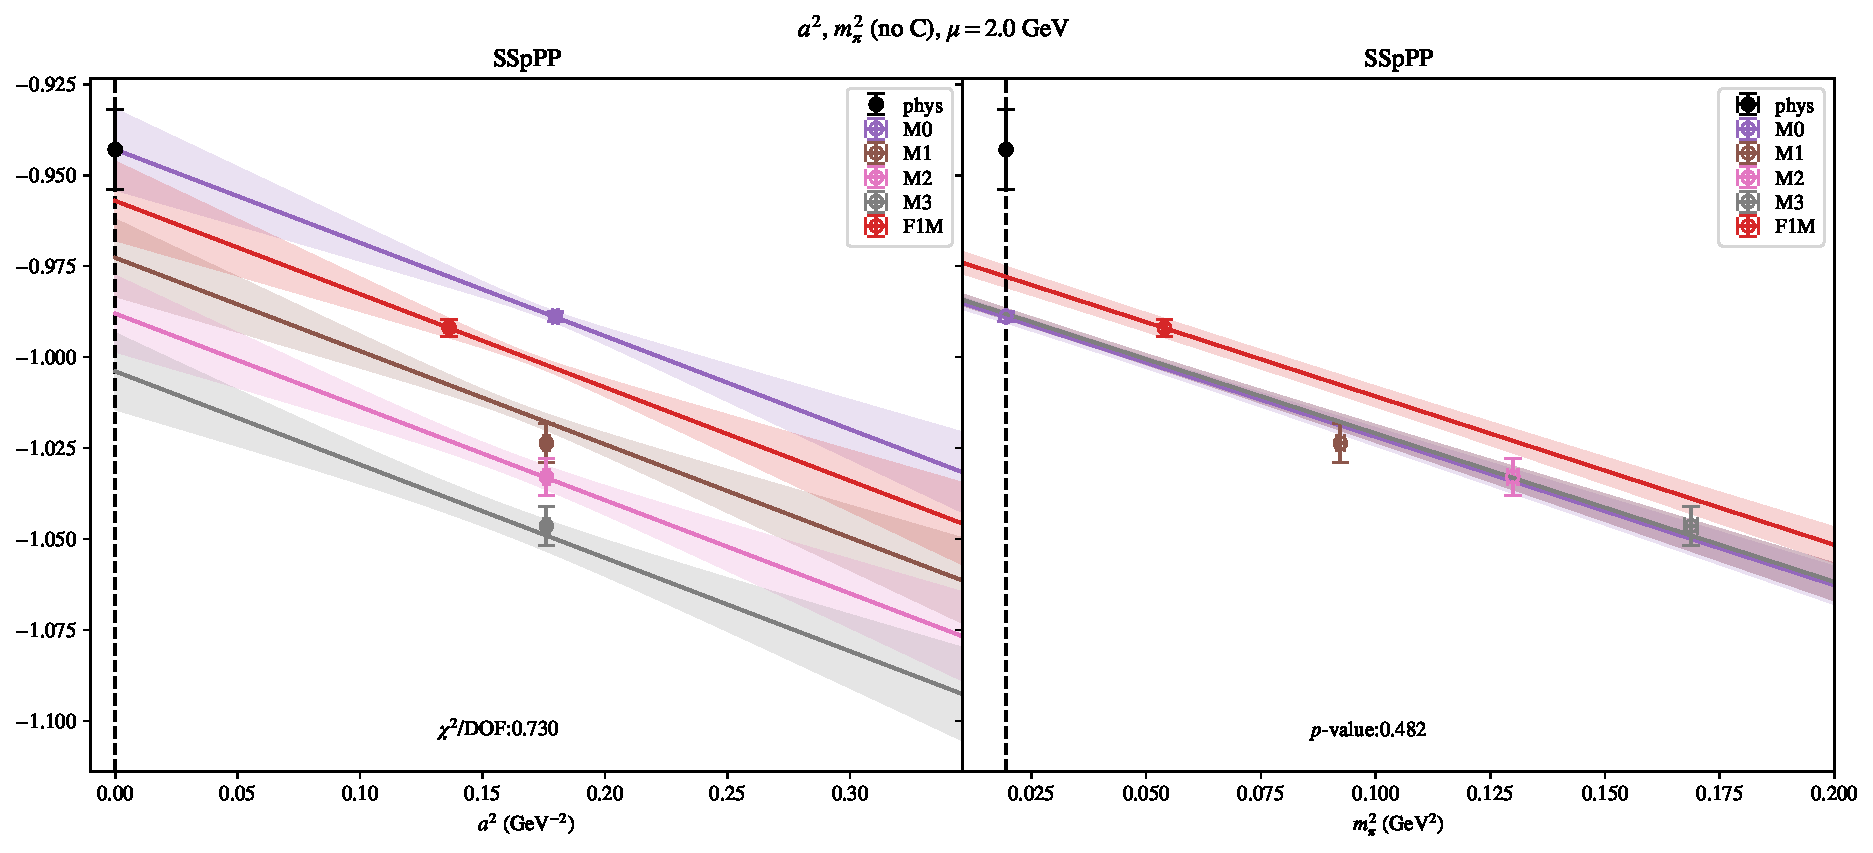
\includepdf[link, pages=-]{VVmAA/SUSY/bag_a2m2noC_20.pdf}
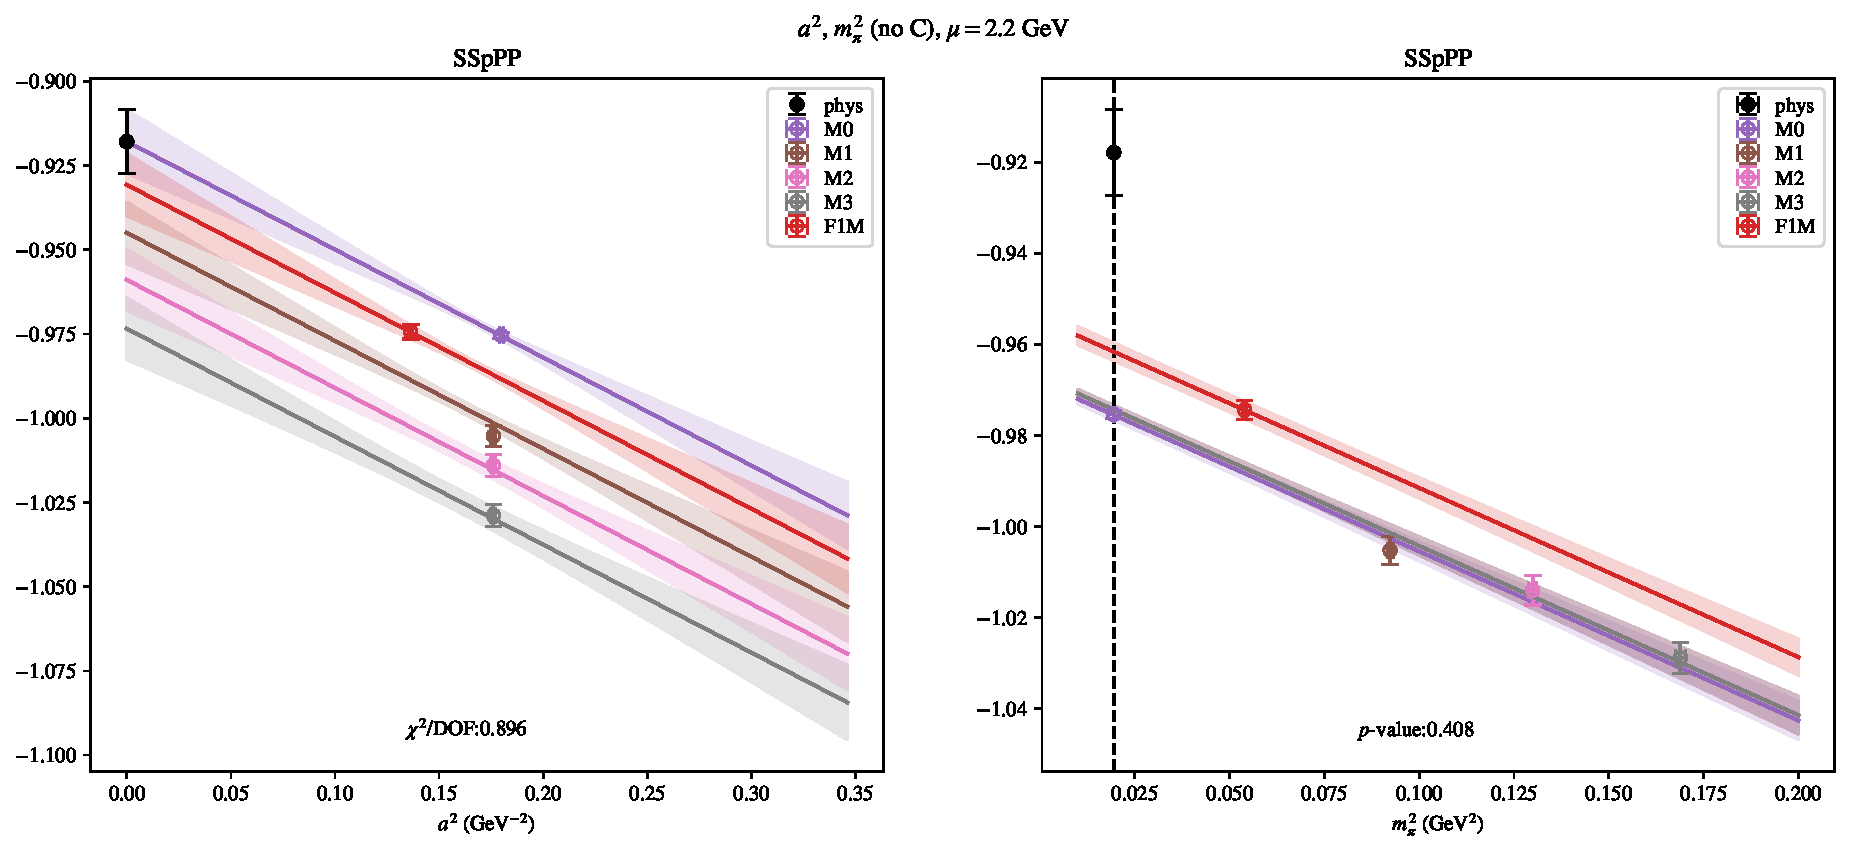
\includepdf[link, pages=-]{VVmAA/SUSY/bag_a2m2noC_22.pdf}
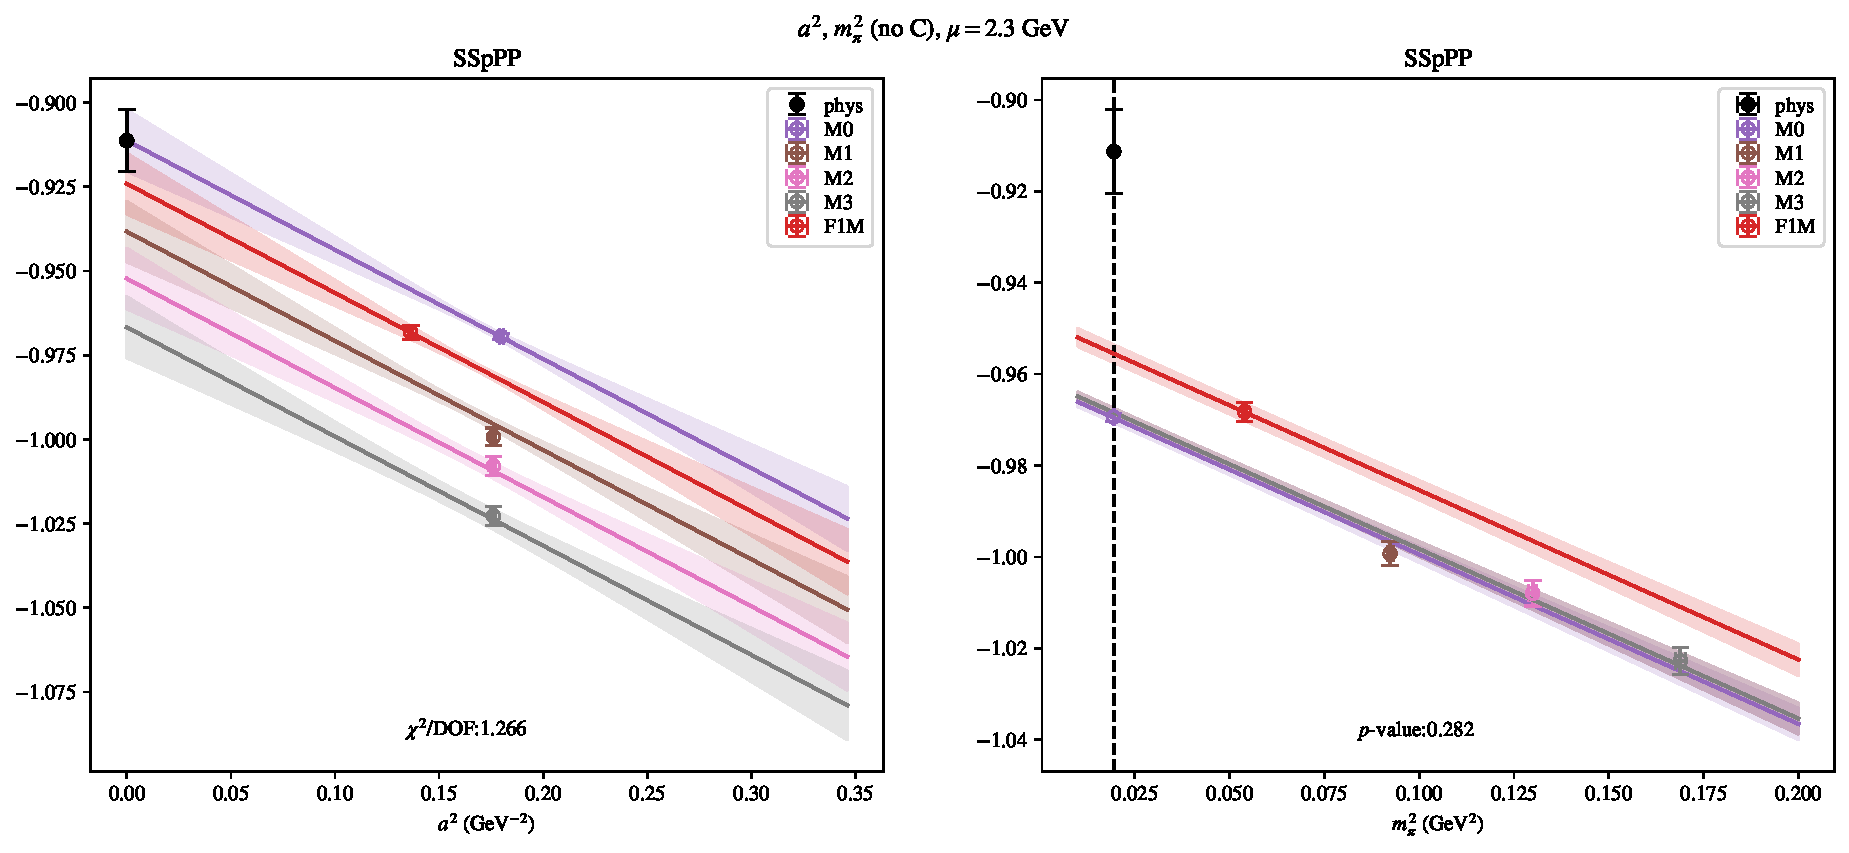
\includepdf[link, pages=-]{VVmAA/SUSY/bag_a2m2noC_23.pdf}
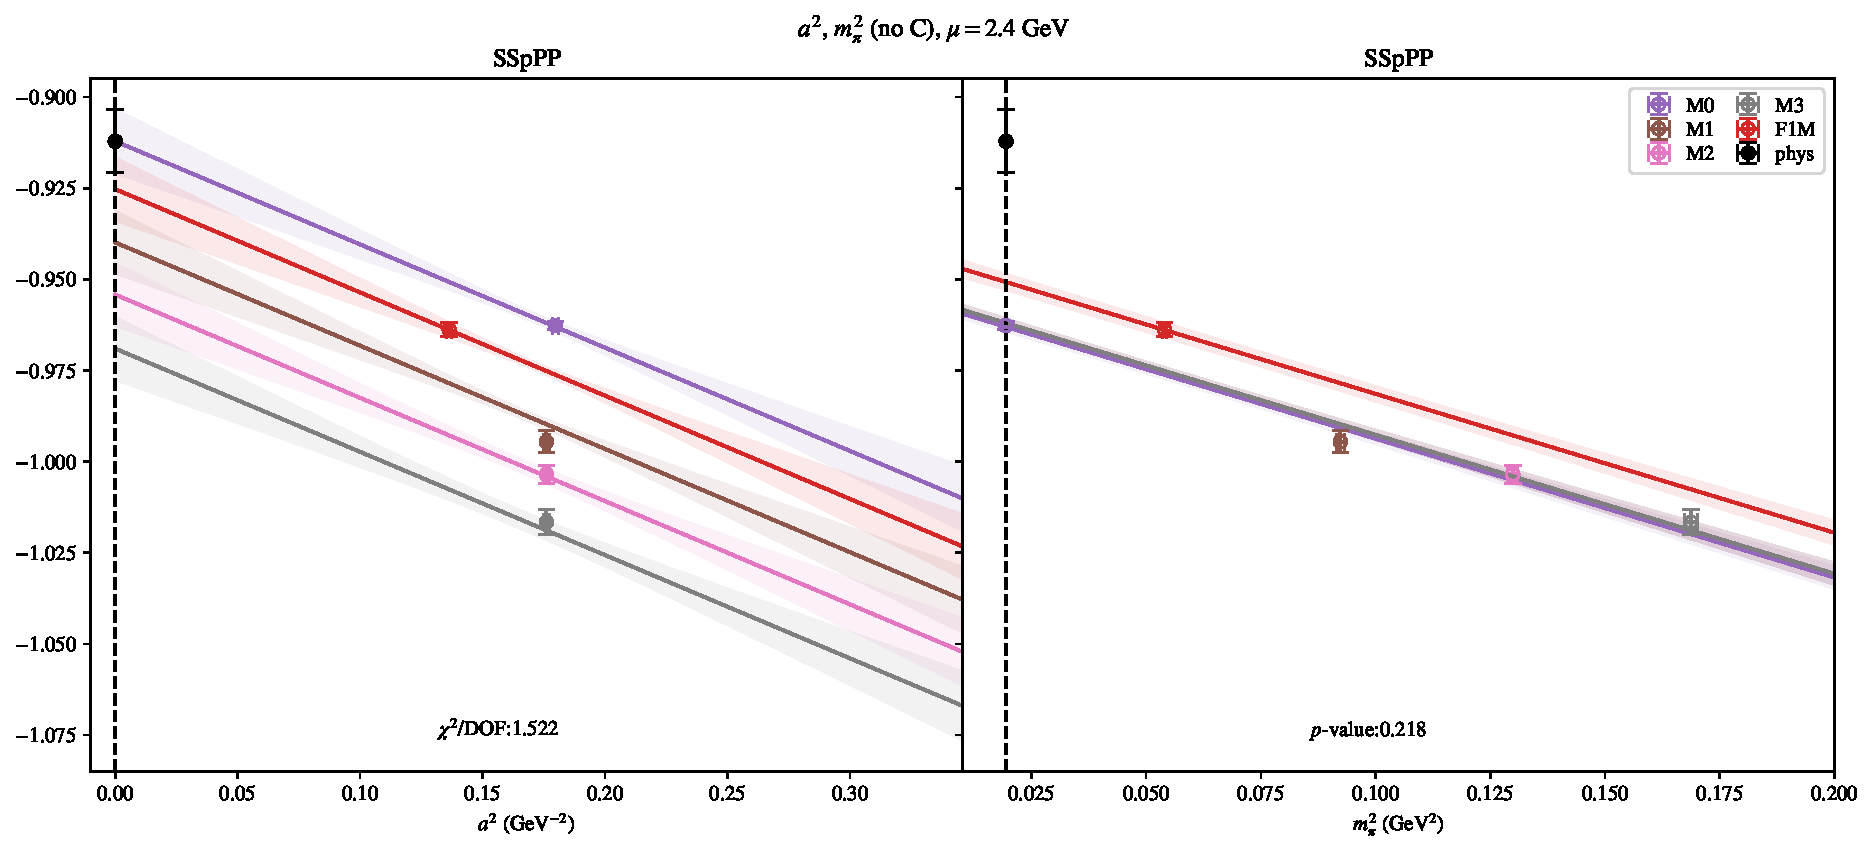
\includepdf[link, pages=-]{VVmAA/SUSY/bag_a2m2noC_24.pdf}
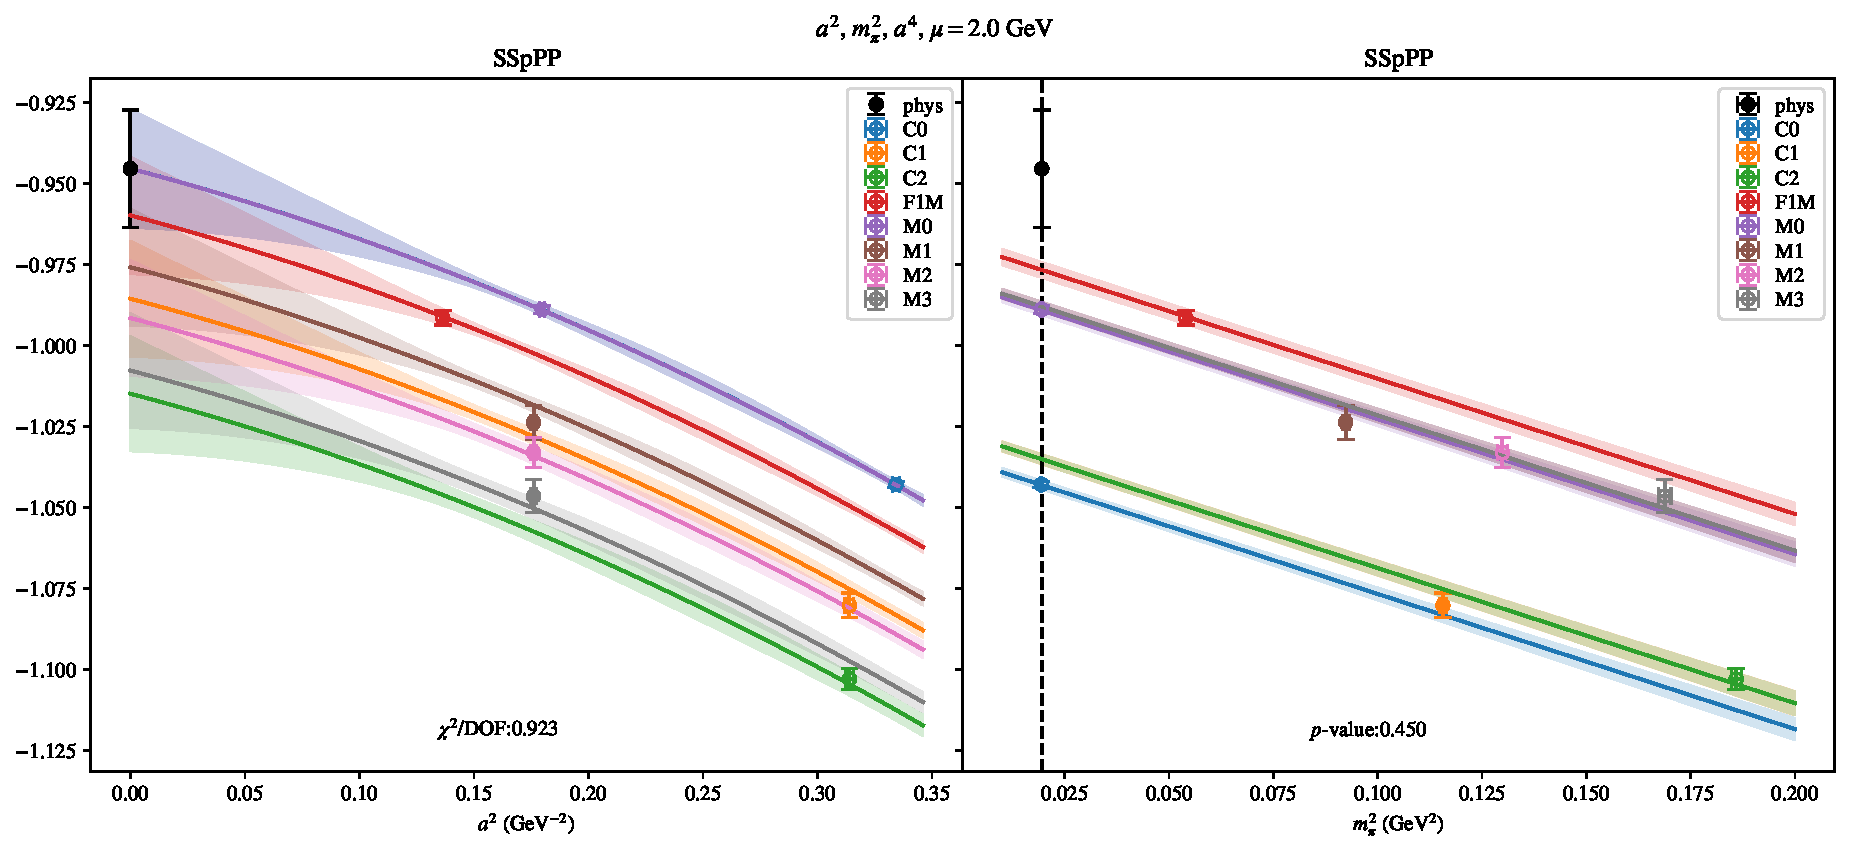
\includepdf[link, pages=-]{VVmAA/SUSY/bag_a2a4m2_20.pdf}
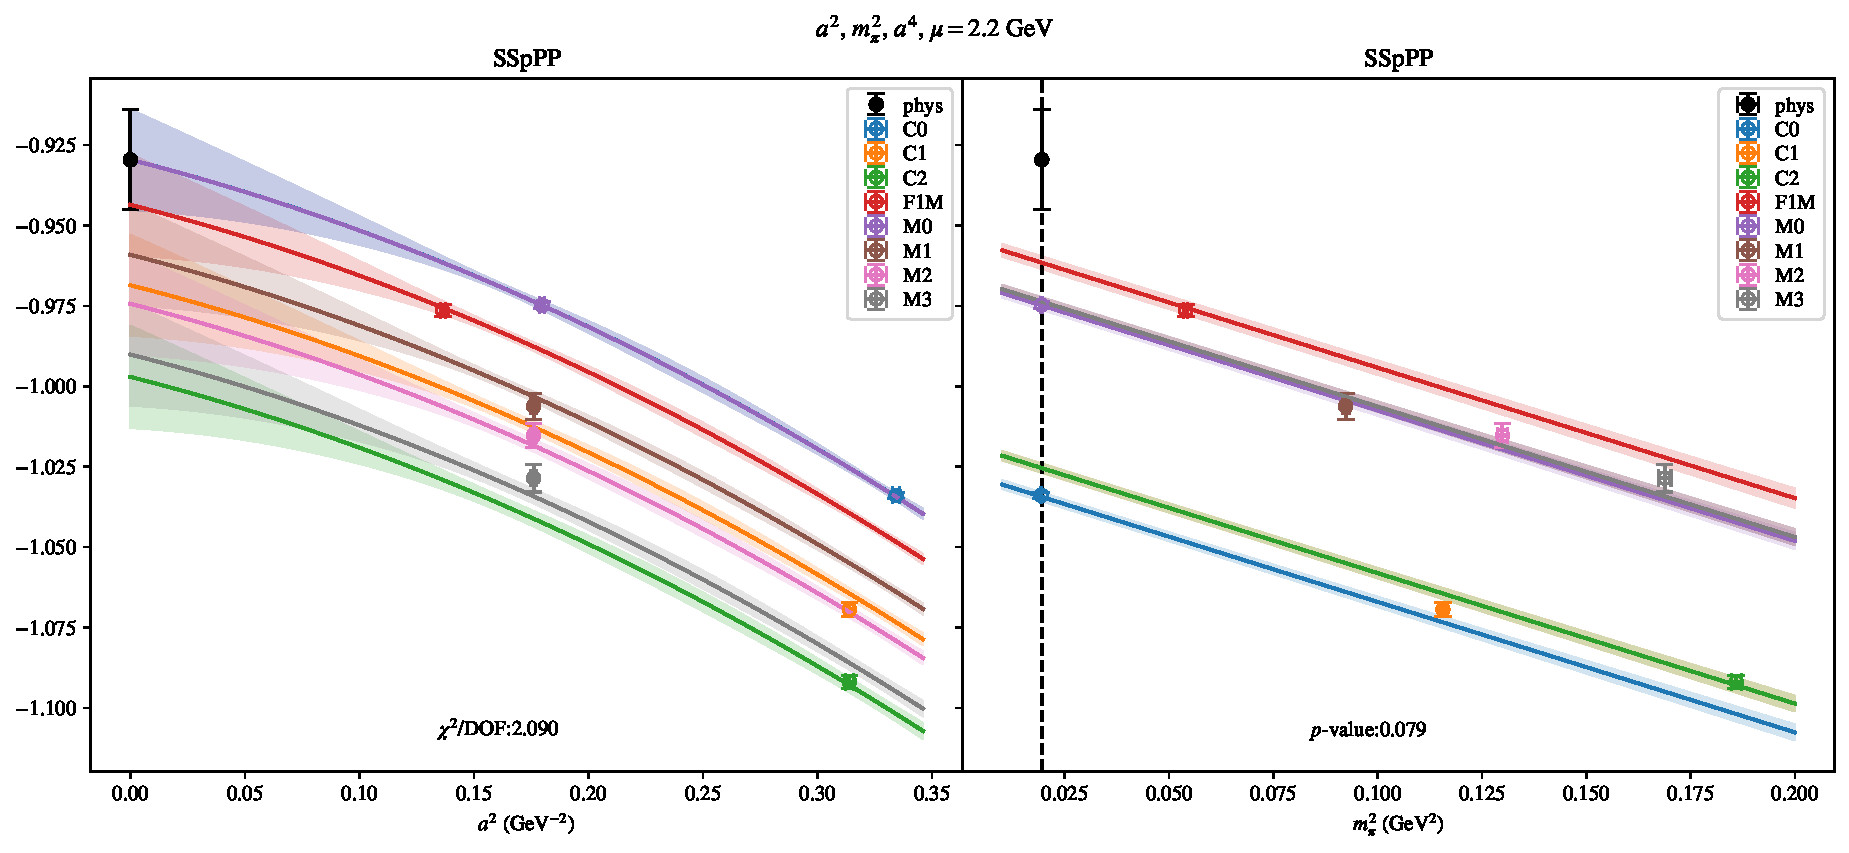
\includepdf[link, pages=-]{VVmAA/SUSY/bag_a2a4m2_22.pdf}
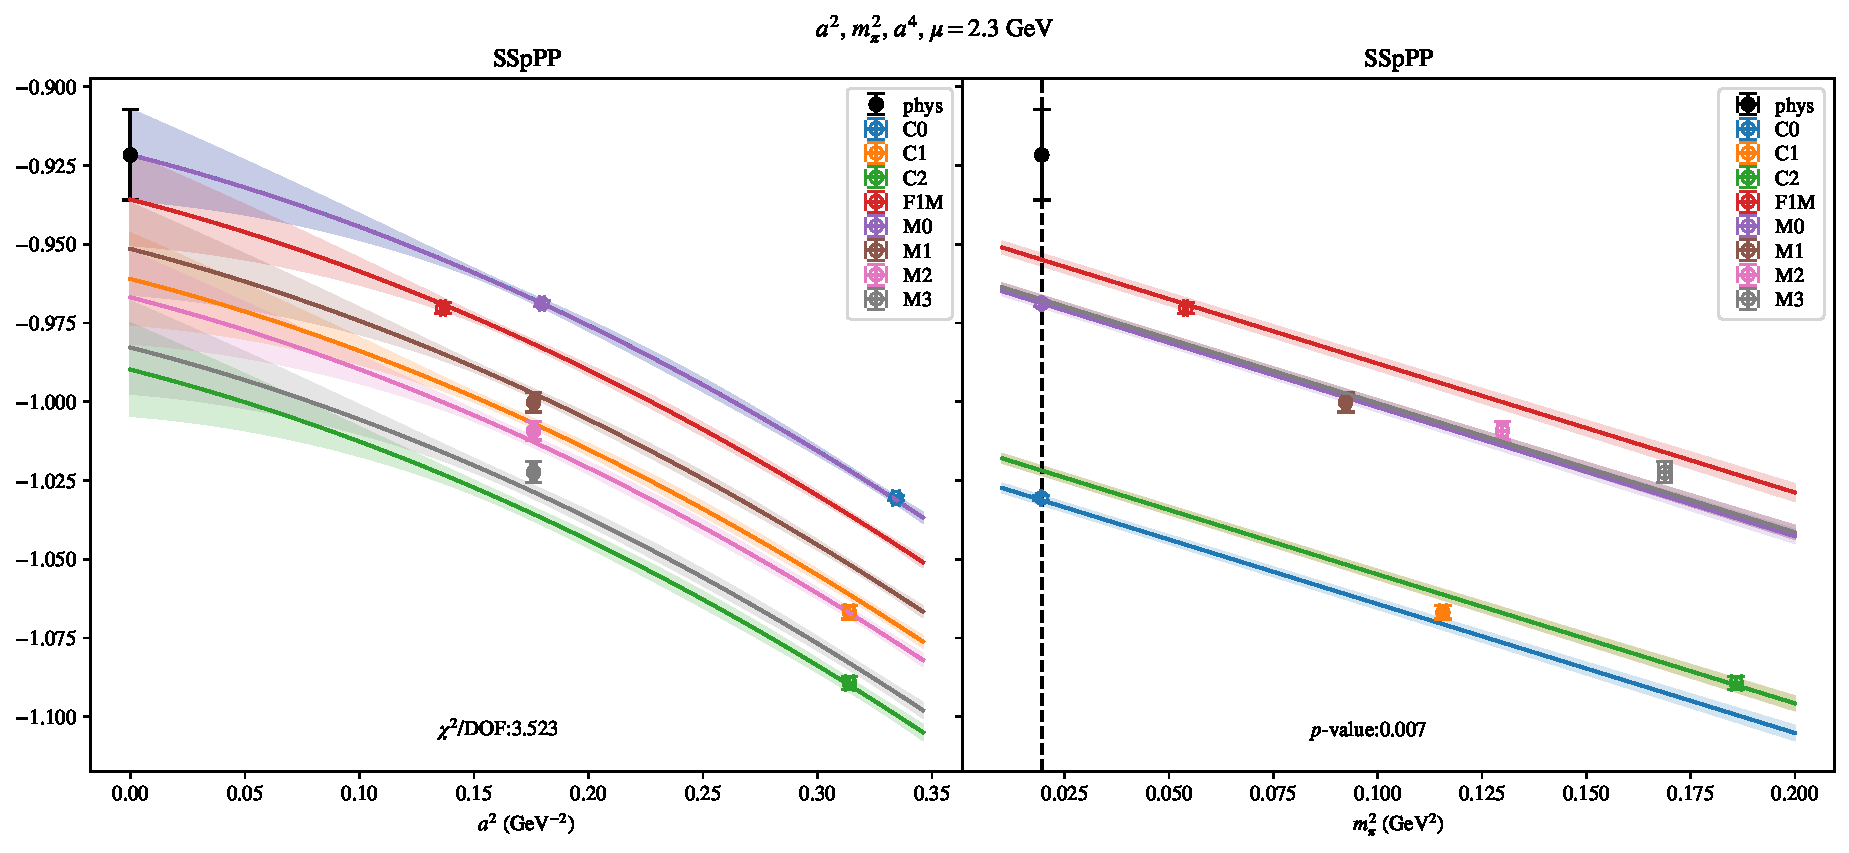
\includepdf[link, pages=-]{VVmAA/SUSY/bag_a2a4m2_23.pdf}
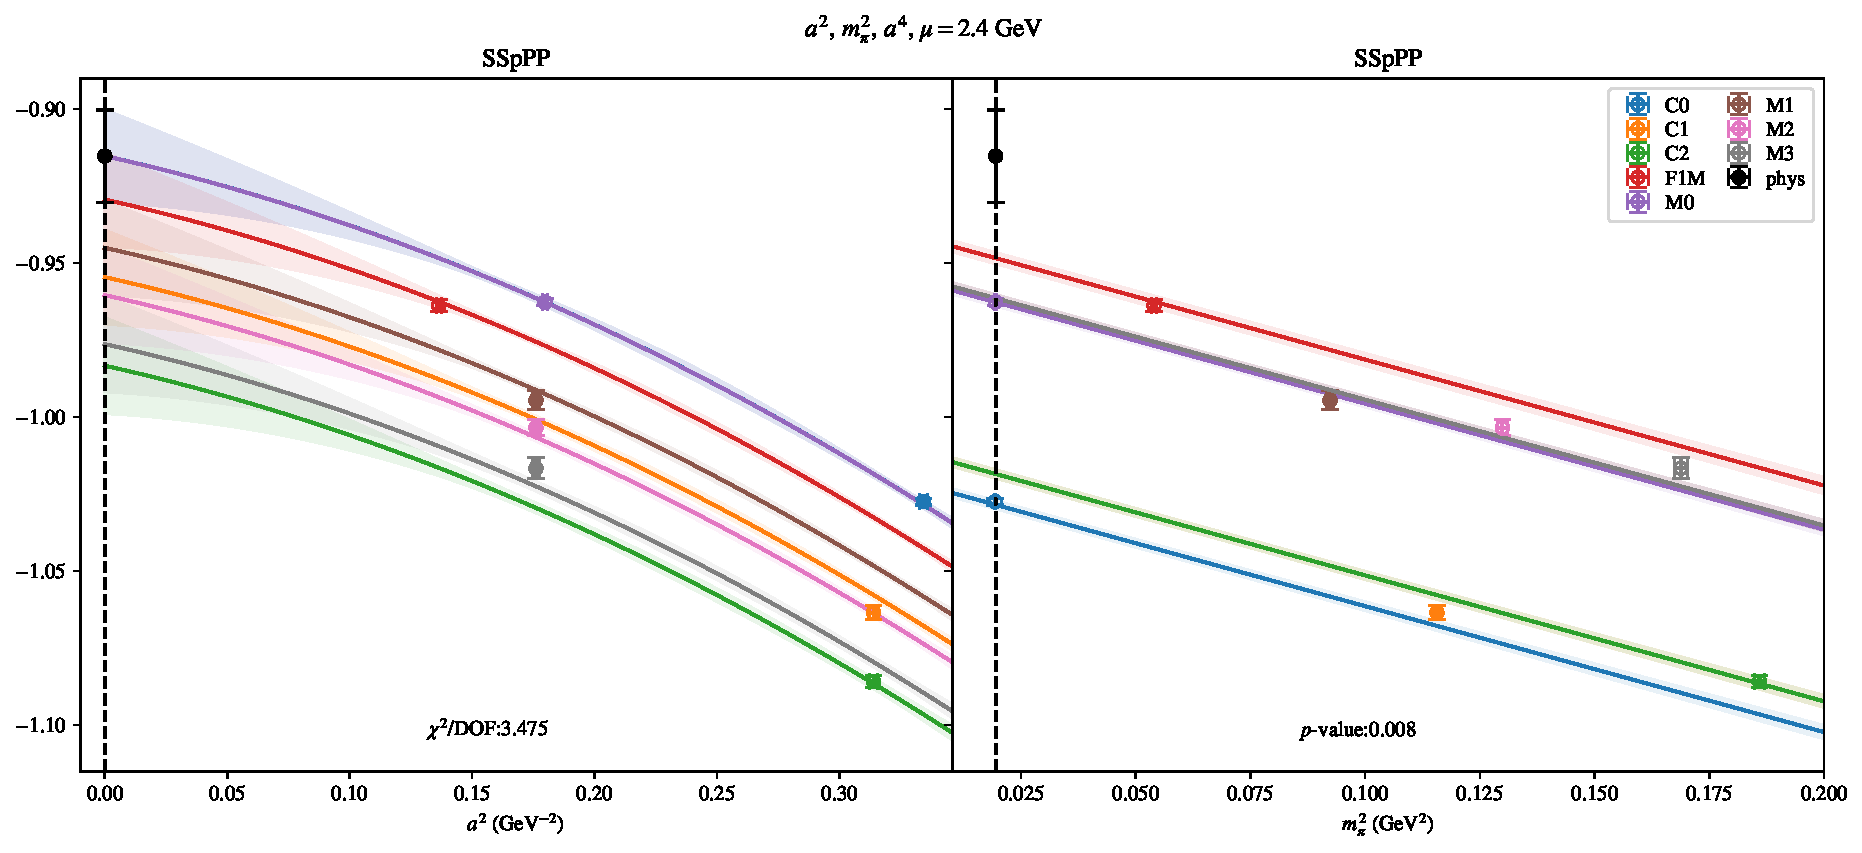
\includepdf[link, pages=-]{VVmAA/SUSY/bag_a2a4m2_24.pdf}
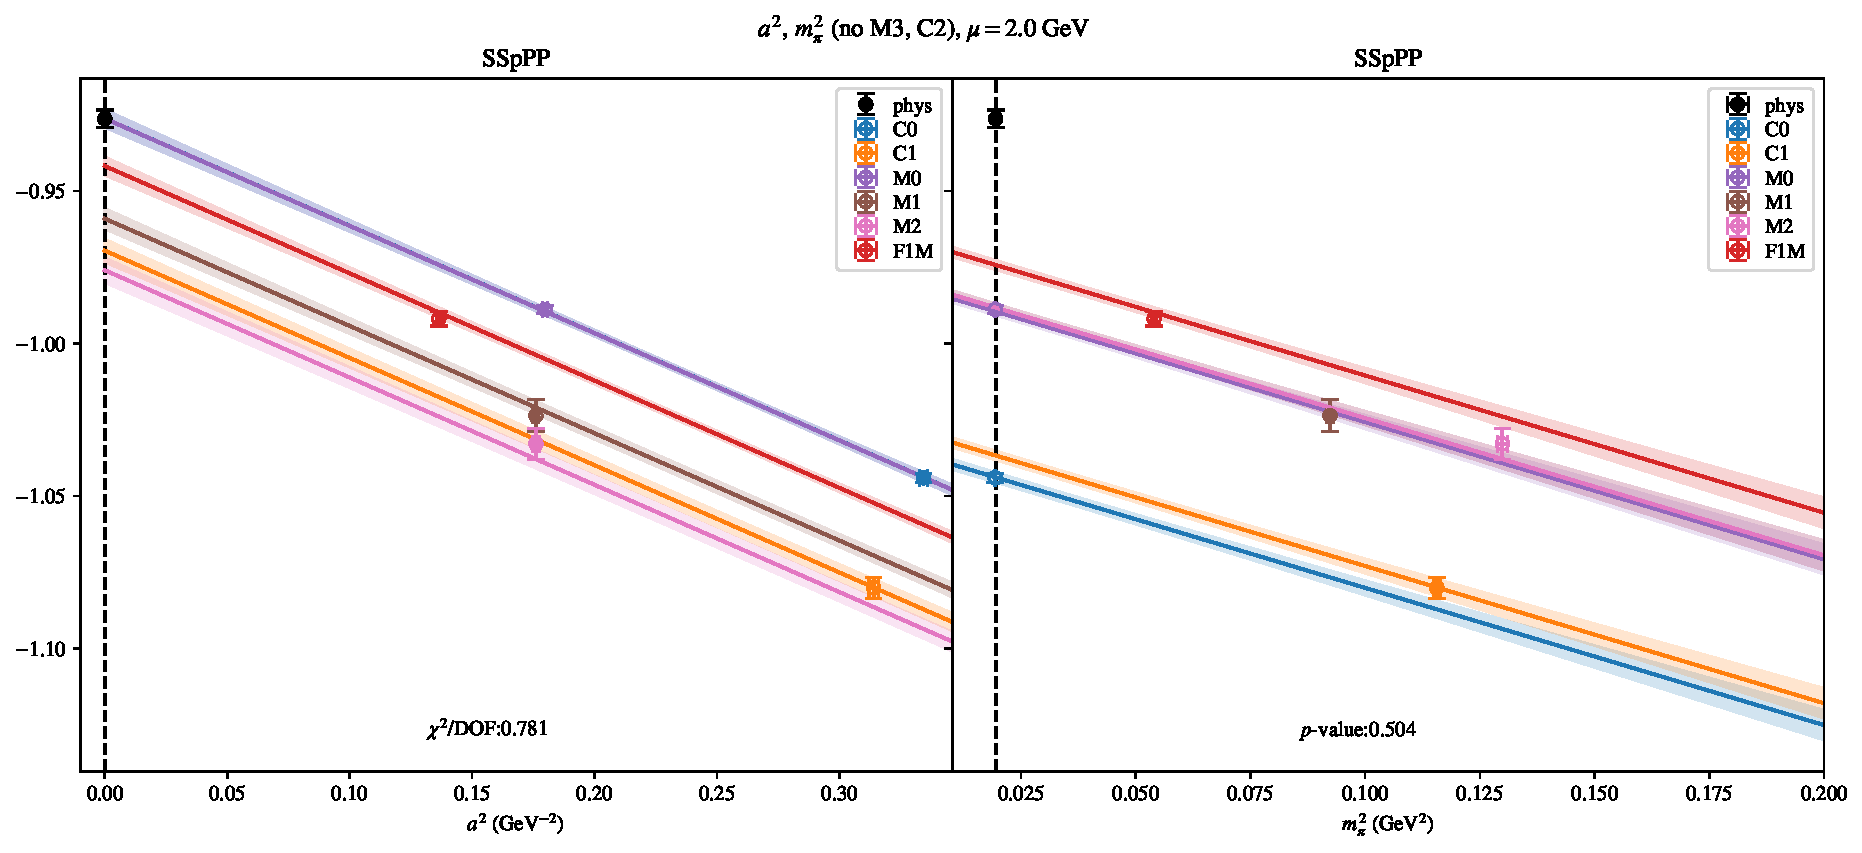
\includepdf[link, pages=-]{VVmAA/SUSY/bag_a2m2mcut_20.pdf}
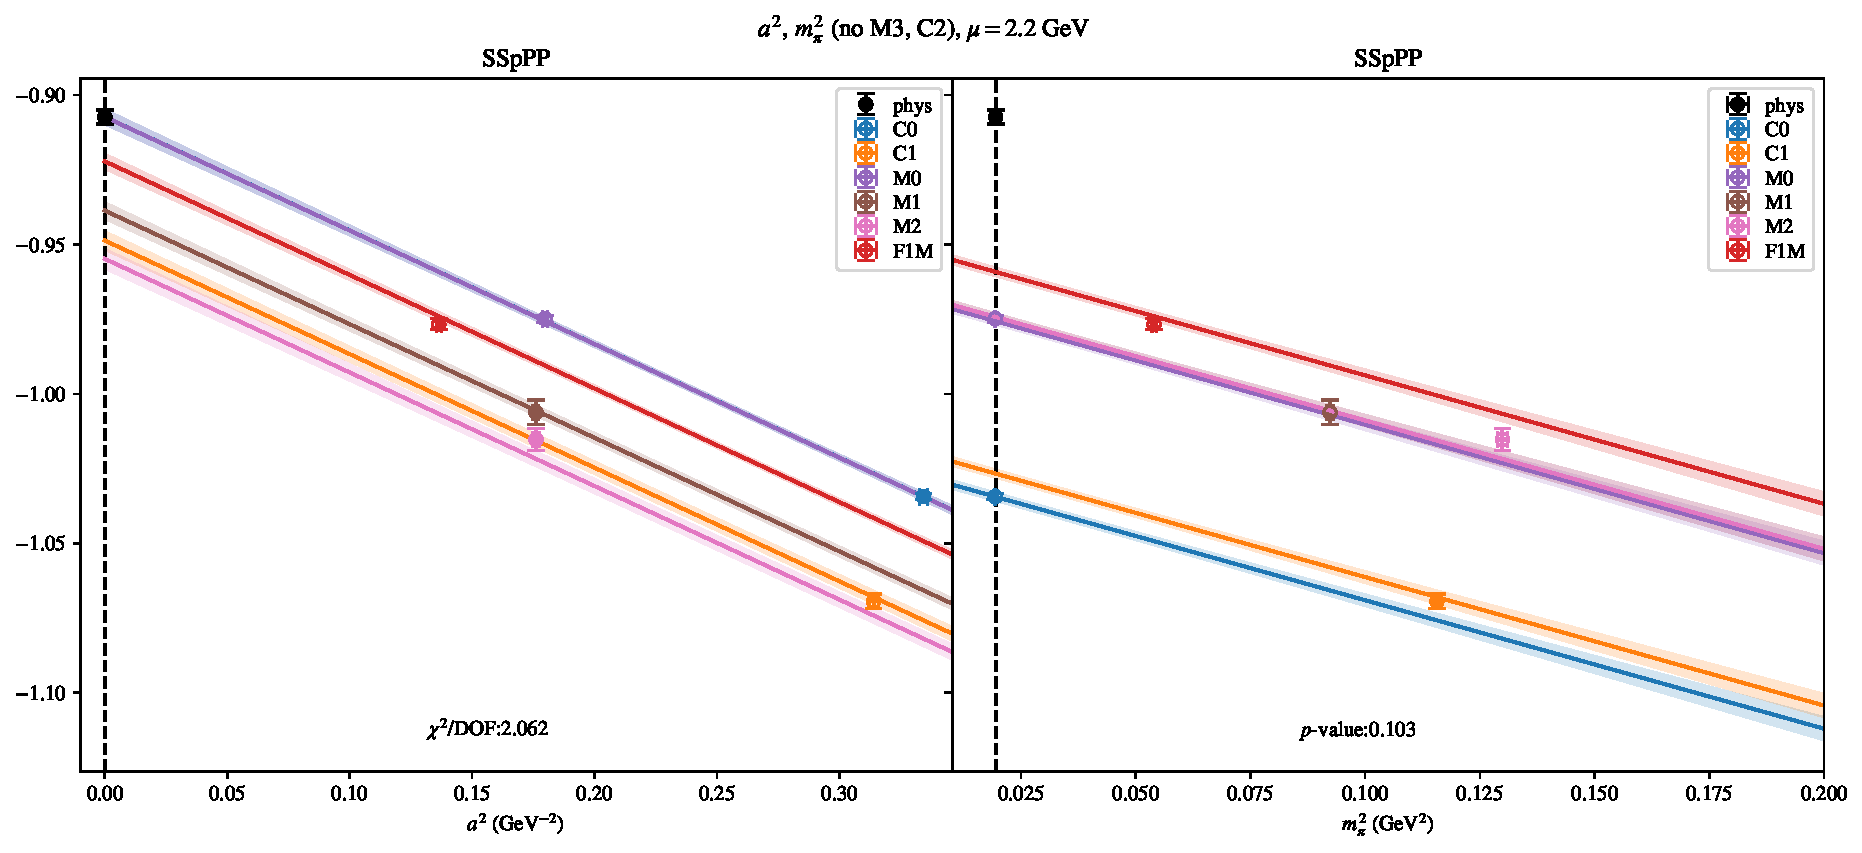
\includepdf[link, pages=-]{VVmAA/SUSY/bag_a2m2mcut_22.pdf}
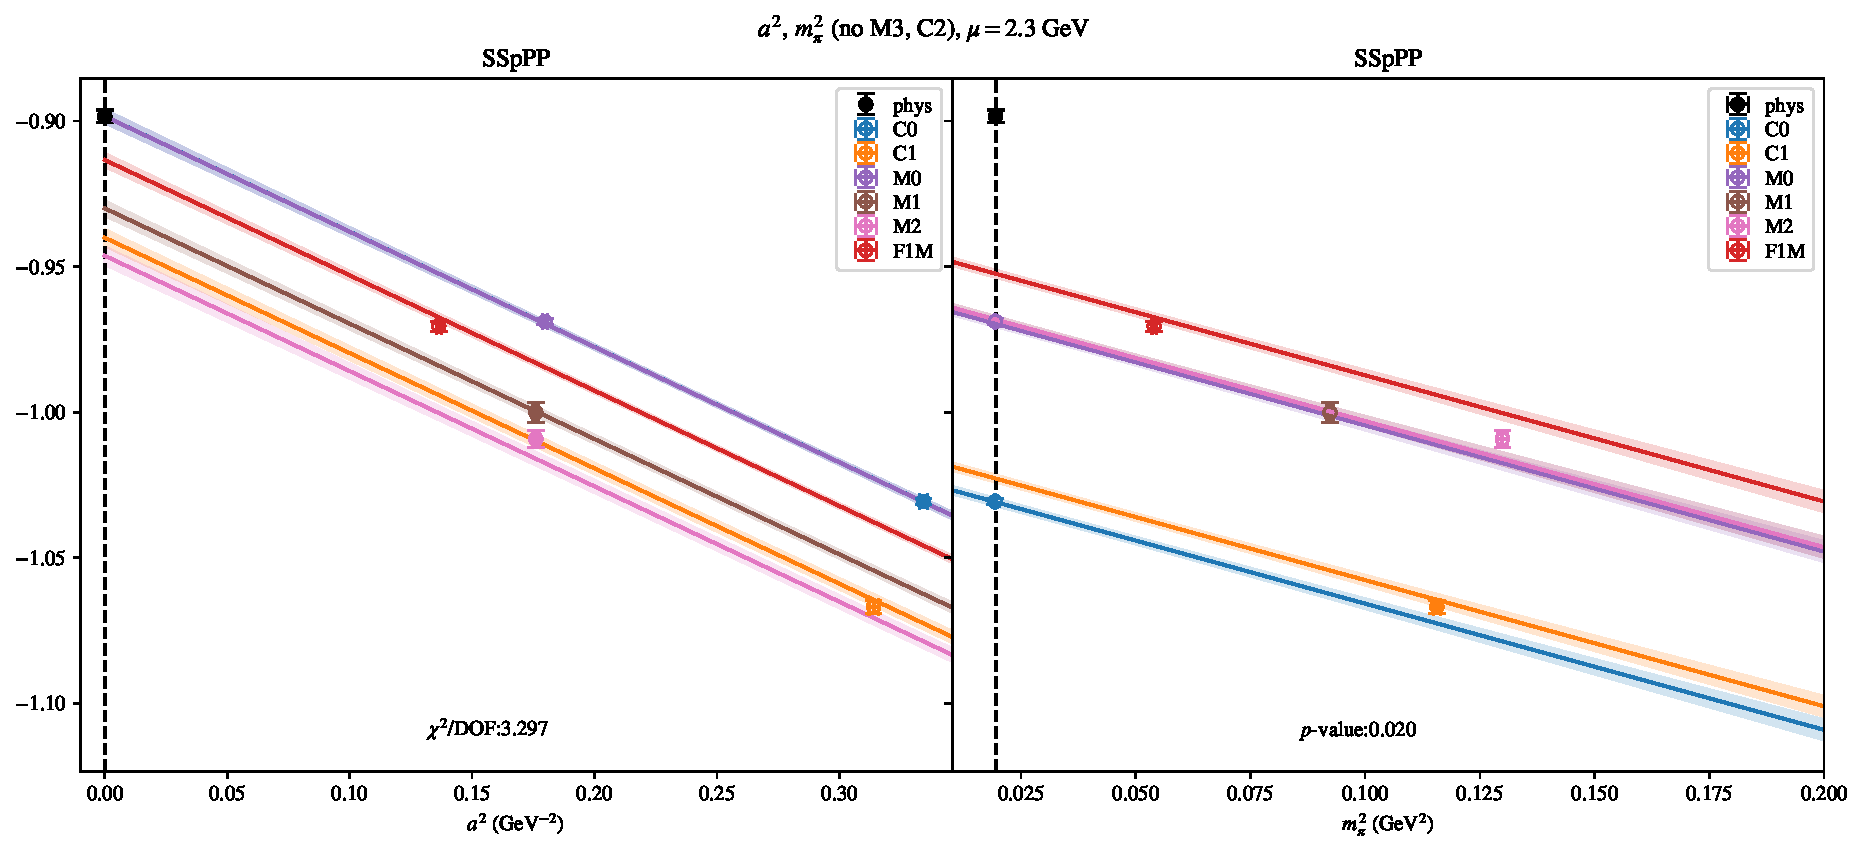
\includepdf[link, pages=-]{VVmAA/SUSY/bag_a2m2mcut_23.pdf}
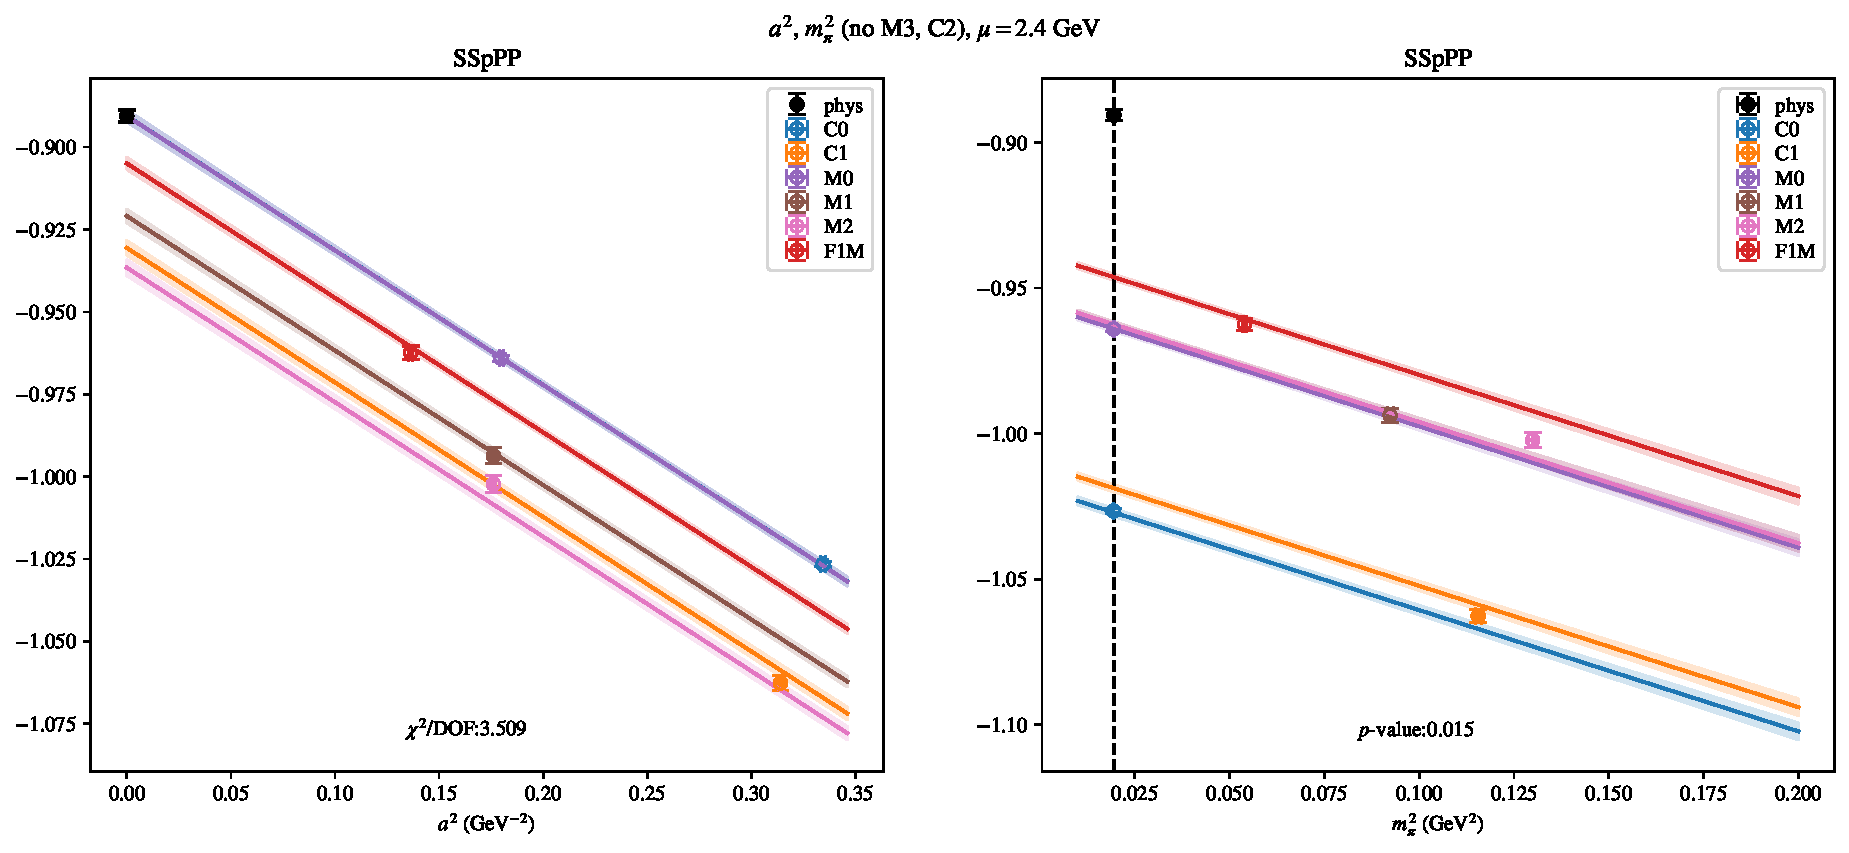
\includepdf[link, pages=-]{VVmAA/SUSY/bag_a2m2mcut_24.pdf}
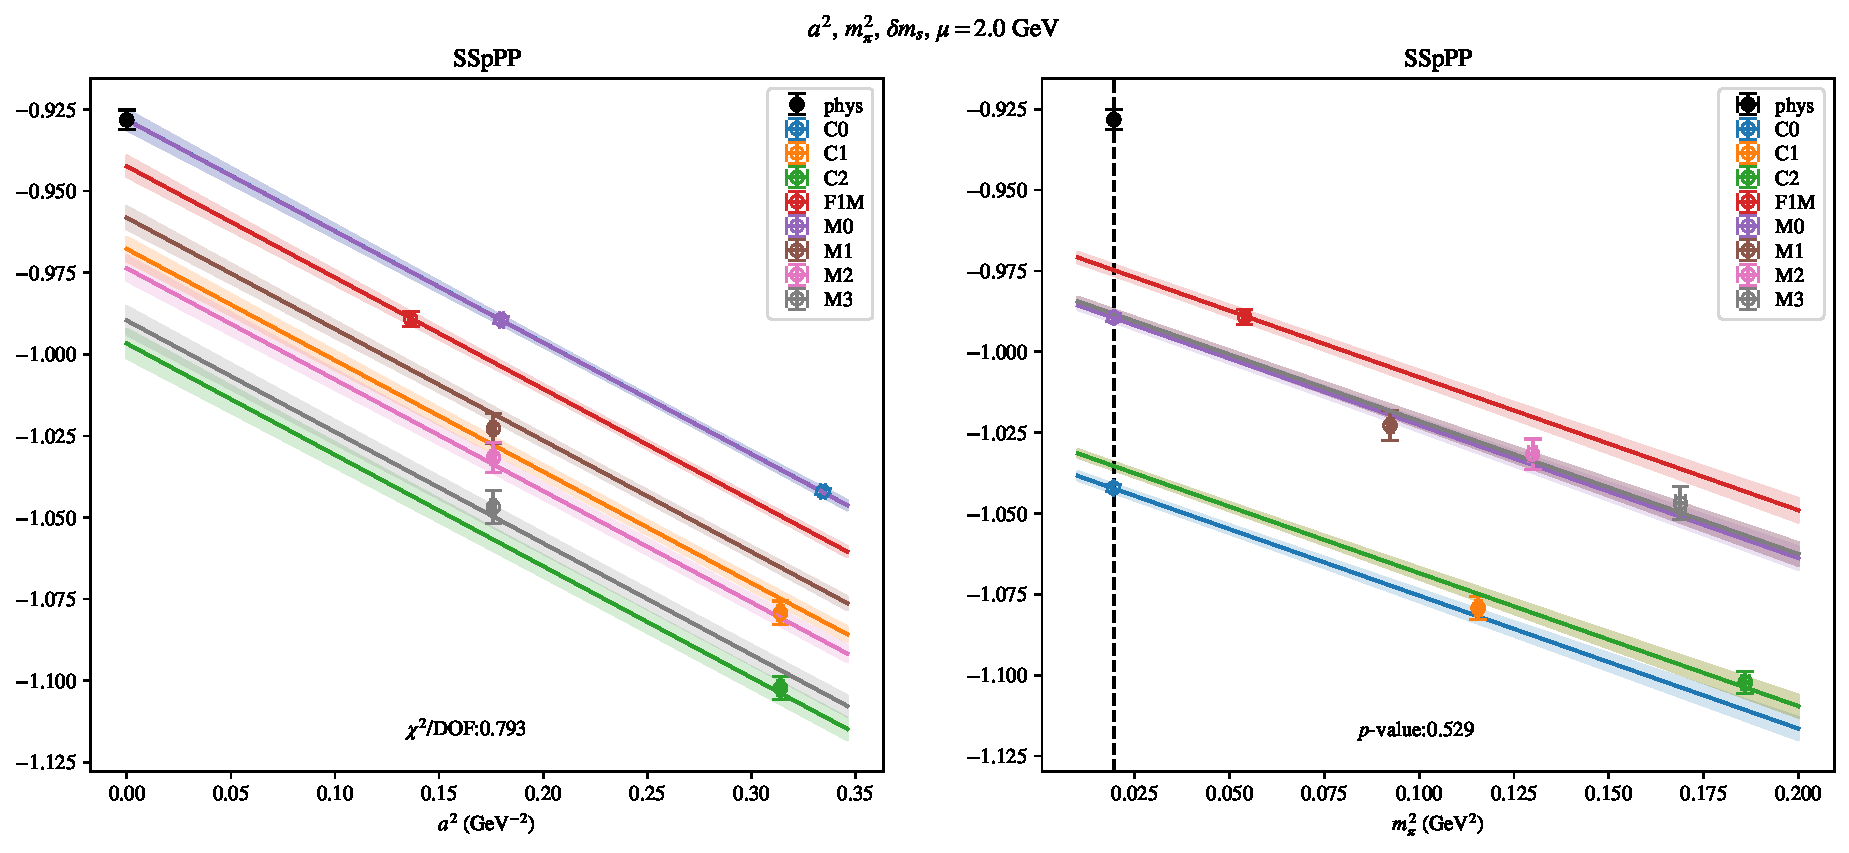
\includepdf[link, pages=-]{VVmAA/SUSY/bag_a2m2delm_20.pdf}
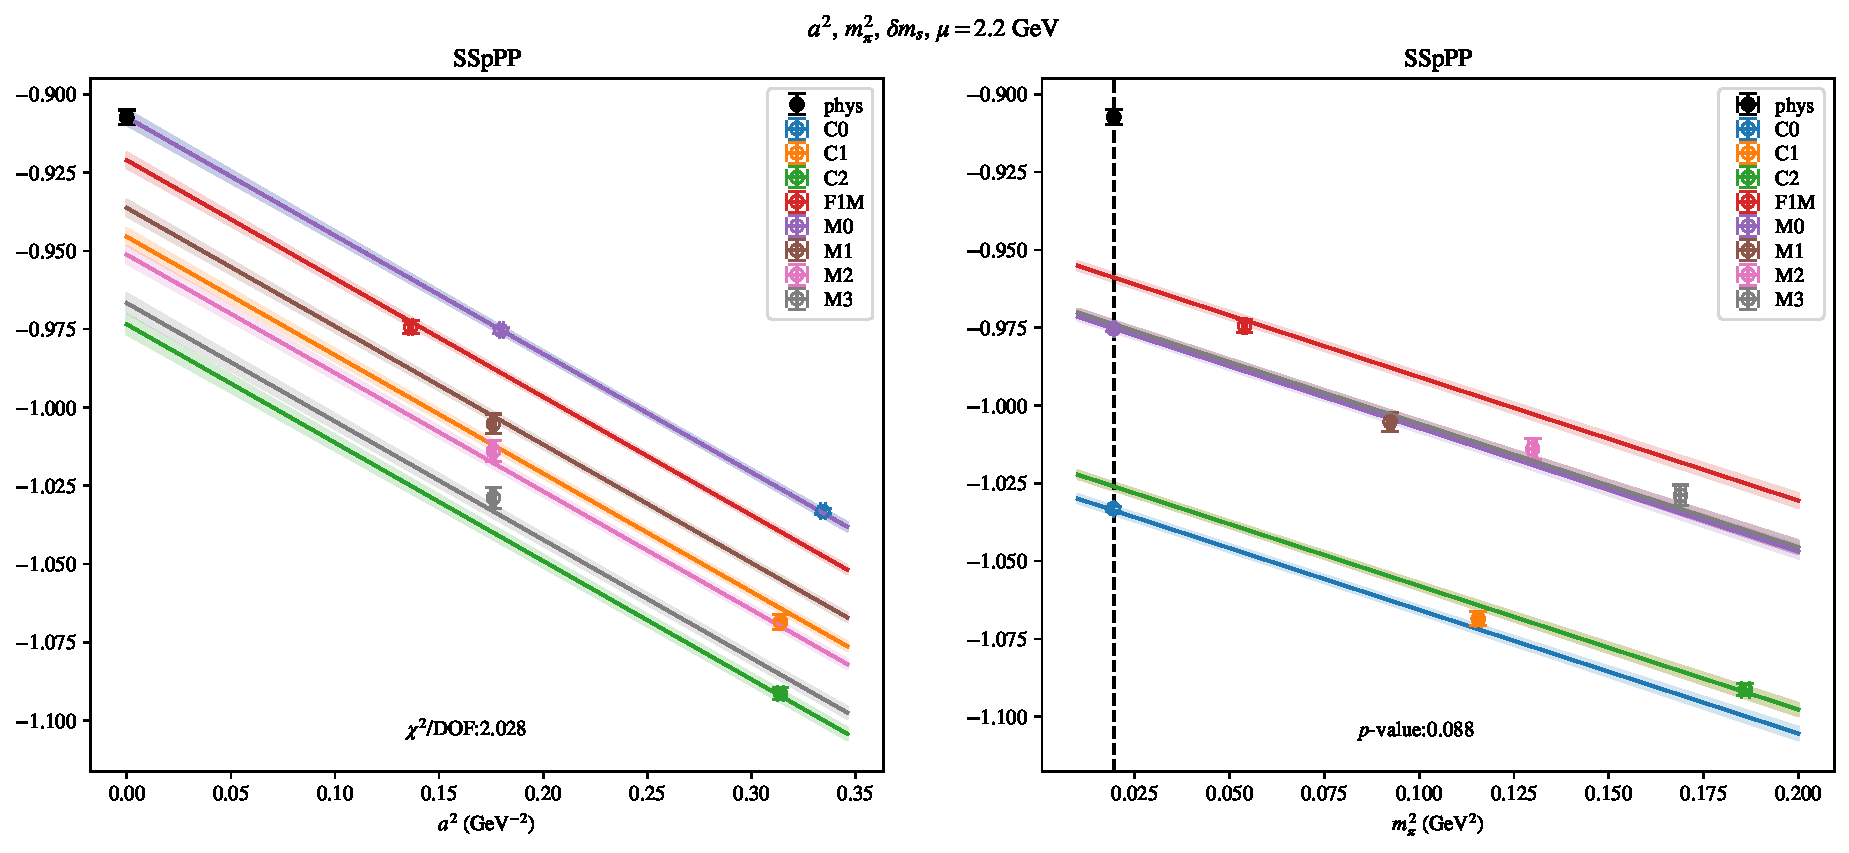
\includepdf[link, pages=-]{VVmAA/SUSY/bag_a2m2delm_22.pdf}
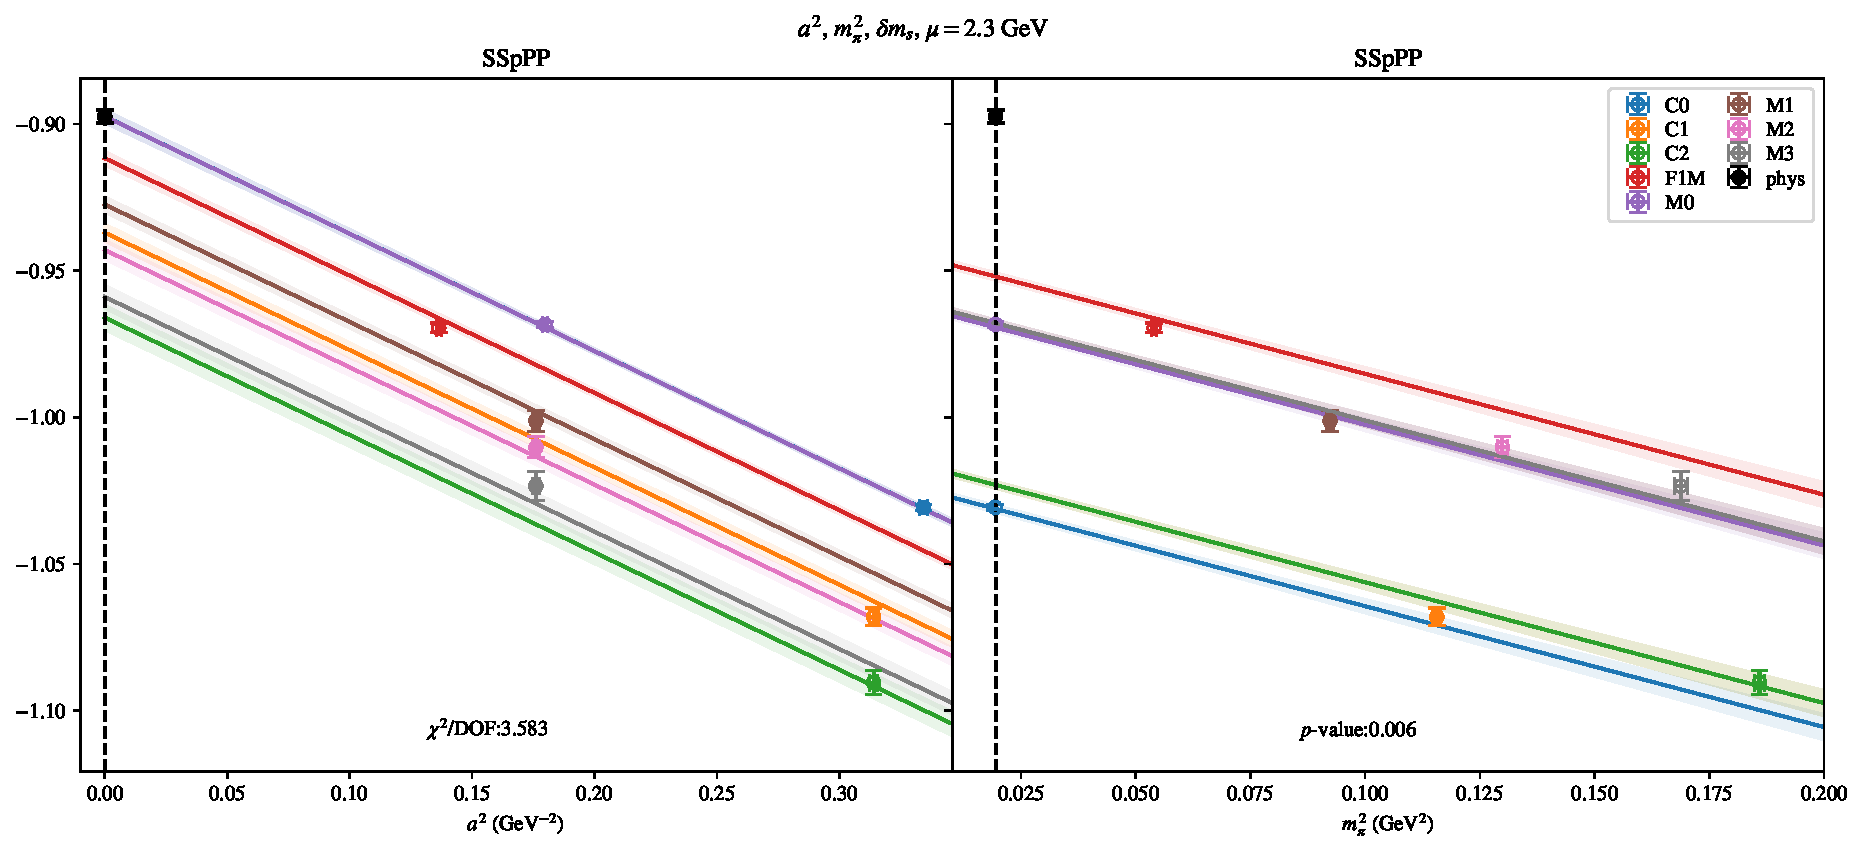
\includepdf[link, pages=-]{VVmAA/SUSY/bag_a2m2delm_23.pdf}
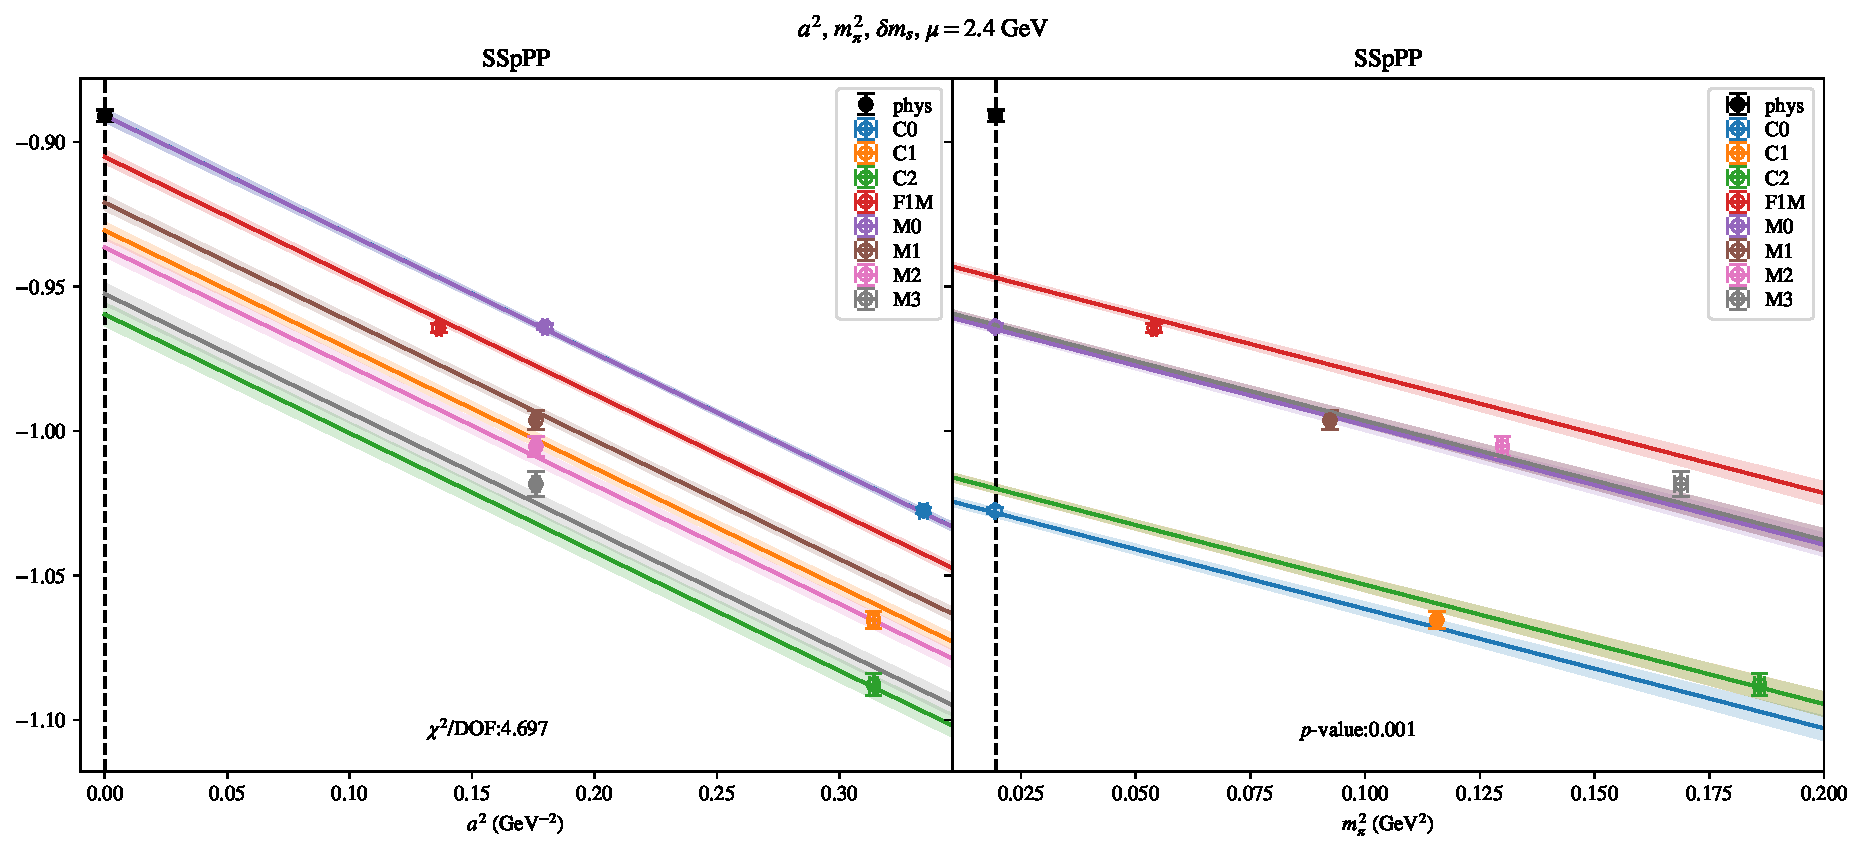
\includepdf[link, pages=-]{VVmAA/SUSY/bag_a2m2delm_24.pdf}
\clearpage
\section{$\mathcal{B}_3$}
\begin{table}[h!]
\begin{center}
\begin{tabular}{|c|c|c|c|c|c|}
\hline
$\mu$ (GeV) & $a^2$, $m_\pi^2$& $a^2$, $m_\pi^2$ (no C)& $a^2$, $m_\pi^2$, $a^4$& $a^2$, $m_\pi^2$ (no M3, C2)& $a^2$, $m_\pi^2$, $\delta m_s$\\
\hline
2.0& \hyperlink{SSmPP/SUSY/bag_a2m2_20.pdf.1}{\textbf{0.2829(56)}: 0.03 (1.0)} & \hyperlink{SSmPP/SUSY/bag_a2m2noC_20.pdf.1}{\textbf{0.286(21)}: 0.033 (0.967)} & \hyperlink{SSmPP/SUSY/bag_a2a4m2_20.pdf.1}{\textbf{0.287(36)}: 0.034 (0.998)} & \hyperlink{SSmPP/SUSY/bag_a2m2mcut_20.pdf.1}{\textbf{0.2824(59)}: 0.016 (0.997)} & \hyperlink{SSmPP/SUSY/bag_a2m2delm_20.pdf.1}{\textbf{0.2829(56)}: 0.037 (0.997)}\\
2.2& \hyperlink{SSmPP/SUSY/bag_a2m2_22.pdf.1}{\textbf{0.2743(46)}: 0.051 (0.998)} & \hyperlink{SSmPP/SUSY/bag_a2m2noC_22.pdf.1}{\textbf{0.279(19)}: 0.037 (0.964)} & \hyperlink{SSmPP/SUSY/bag_a2a4m2_22.pdf.1}{\textbf{0.280(31)}: 0.056 (0.994)} & \hyperlink{SSmPP/SUSY/bag_a2m2mcut_22.pdf.1}{\textbf{0.2740(49)}: 0.039 (0.99)} & \hyperlink{SSmPP/SUSY/bag_a2m2delm_22.pdf.1}{\textbf{0.2743(46)}: 0.064 (0.992)}\\
2.3& \hyperlink{SSmPP/SUSY/bag_a2m2_23.pdf.1}{\textbf{0.2704(42)}: 0.068 (0.997)} & \hyperlink{SSmPP/SUSY/bag_a2m2noC_23.pdf.1}{\textbf{0.277(17)}: 0.037 (0.963)} & \hyperlink{SSmPP/SUSY/bag_a2a4m2_23.pdf.1}{\textbf{0.278(27)}: 0.068 (0.992)} & \hyperlink{SSmPP/SUSY/bag_a2m2mcut_23.pdf.1}{\textbf{0.2702(44)}: 0.053 (0.984)} & \hyperlink{SSmPP/SUSY/bag_a2m2delm_23.pdf.1}{\textbf{0.2704(42)}: 0.084 (0.987)}\\
2.4& \hyperlink{SSmPP/SUSY/bag_a2m2_24.pdf.1}{\textbf{0.2671(37)}: 0.101 (0.992)} & \hyperlink{SSmPP/SUSY/bag_a2m2noC_24.pdf.1}{\textbf{0.274(15)}: 0.048 (0.953)} & \hyperlink{SSmPP/SUSY/bag_a2a4m2_24.pdf.1}{\textbf{0.275(26)}: 0.102 (0.982)} & \hyperlink{SSmPP/SUSY/bag_a2m2mcut_24.pdf.1}{\textbf{0.2669(39)}: 0.09 (0.966)} & \hyperlink{SSmPP/SUSY/bag_a2m2delm_24.pdf.1}{\textbf{0.2671(37)}: 0.124 (0.974)}\\
\hline
\end{tabular}
\caption{Physical point value from chiral and continuum extrapolation at renormalisation scale $\mu$. Entries are \textbf{value(error)}: $\chi^2/\text{DOF}$ ($p$-value).}
\end{center}
\end{table}
\begin{table}[h!]
\begin{center}
\begin{tabular}{|c c|c|c|c|c|c|}
\hline
$\mu$ (GeV) &  & $a^2$, $m_\pi^2$& $a^2$, $m_\pi^2$ (no C)& $a^2$, $m_\pi^2$, $a^4$& $a^2$, $m_\pi^2$ (no M3, C2)& $a^2$, $m_\pi^2$, $\delta m_s$\\
\hline
\multirow{3}{0.5in}{2.0} & $\alpha$ & 0.178(20)& 0.16(12)& 0.14(33)& 0.179(21)& 0.178(20)\\
 & $\beta$ & 0.00227(58)& 0.0023(10)& 0.00229(59)& 0.00253(99)& 0.0022(10)\\
 & $\gamma$ &  &  & 0.08(66)&  & 0.002(33)\\
\hline
\multirow{3}{0.5in}{2.2} & $\alpha$ & 0.202(17)& 0.17(11)& 0.15(28)& 0.203(17)& 0.202(17)\\
 & $\beta$ & 0.00221(48)& 0.00211(81)& 0.00223(49)& 0.00243(81)& 0.00221(87)\\
 & $\gamma$ &  &  & 0.11(58)&  & 0.0003(287)\\
\hline
\multirow{3}{0.5in}{2.3} & $\alpha$ & 0.214(15)& 0.177(97)& 0.15(24)& 0.214(16)& 0.214(15)\\
 & $\beta$ & 0.00223(46)& 0.00209(74)& 0.00225(46)& 0.00247(79)& 0.00228(75)\\
 & $\gamma$ &  &  & 0.14(50)&  & -0.002(25)\\
\hline
\multirow{3}{0.5in}{2.4} & $\alpha$ & 0.225(13)& 0.185(87)& 0.15(23)& 0.225(14)& 0.225(14)\\
 & $\beta$ & 0.00221(40)& 0.00205(63)& 0.00223(40)& 0.00242(67)& 0.00227(74)\\
 & $\gamma$ &  &  & 0.15(48)&  & -0.003(24)\\
\hline
\end{tabular}
\caption{Fit values of coefficients in $Q = Q_{phys} + \mathbf{\alpha} a^2 + \mathbf{\beta}\left(\frac{m_\pi^2}{f_\pi^2}-\frac{m_{\pi,PDG}^2}{f_\pi^2}\right) + \gamma(\ldots)$}
\end{center}
\end{table}
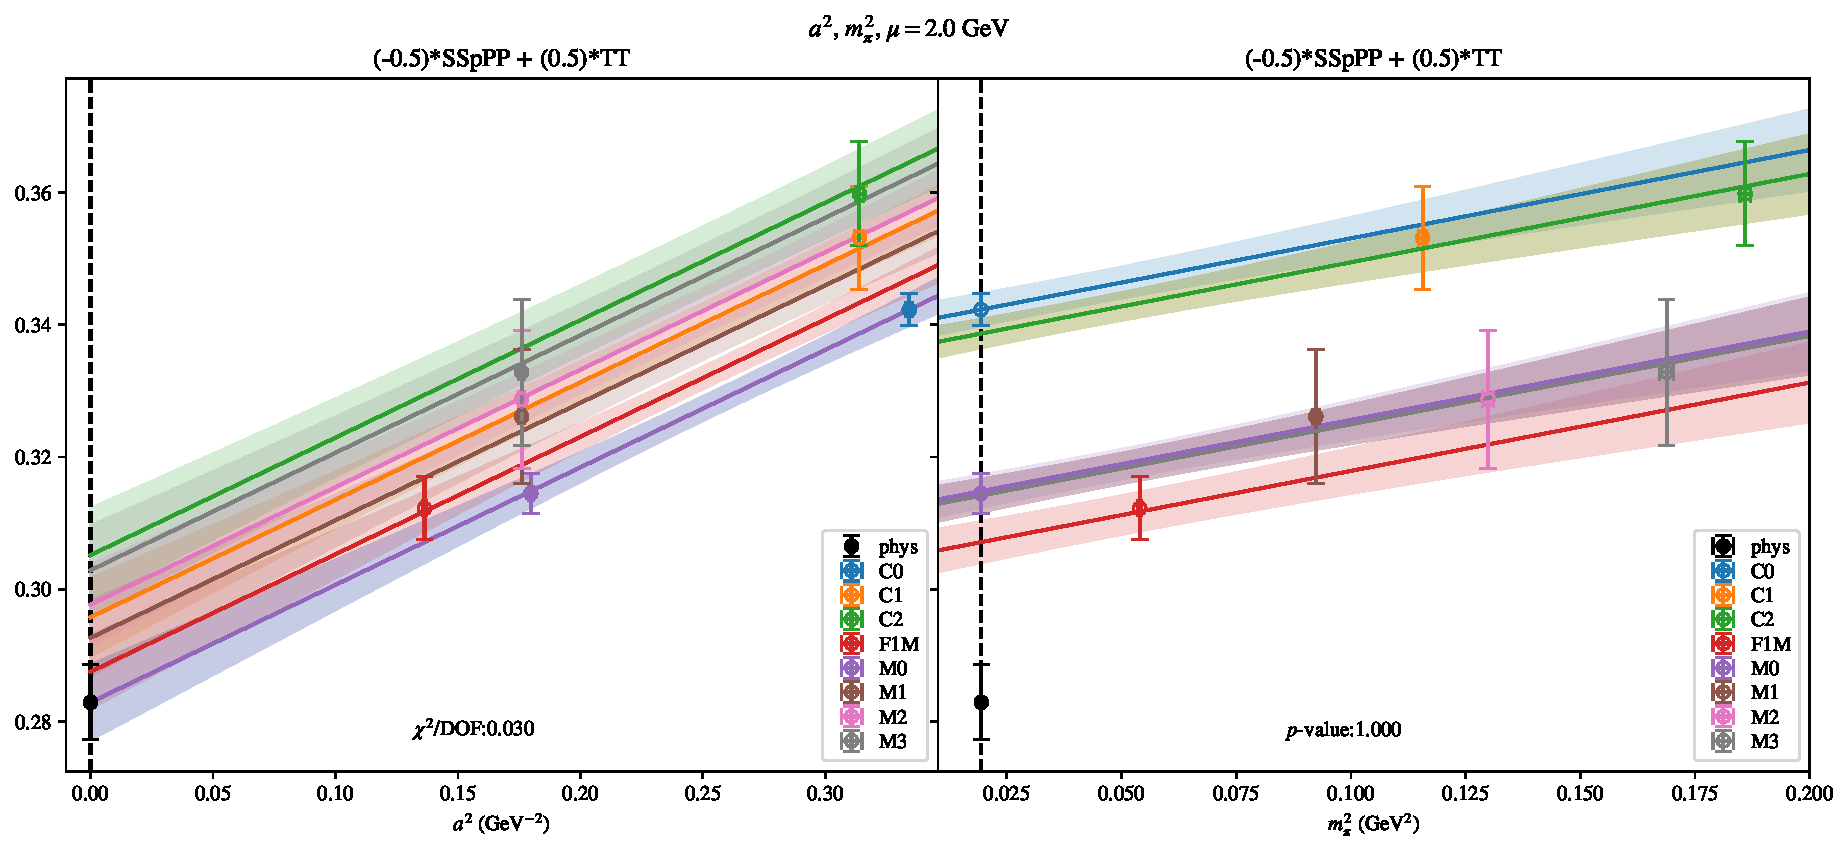
\includepdf[link, pages=-]{SSmPP/SUSY/bag_a2m2_20.pdf}
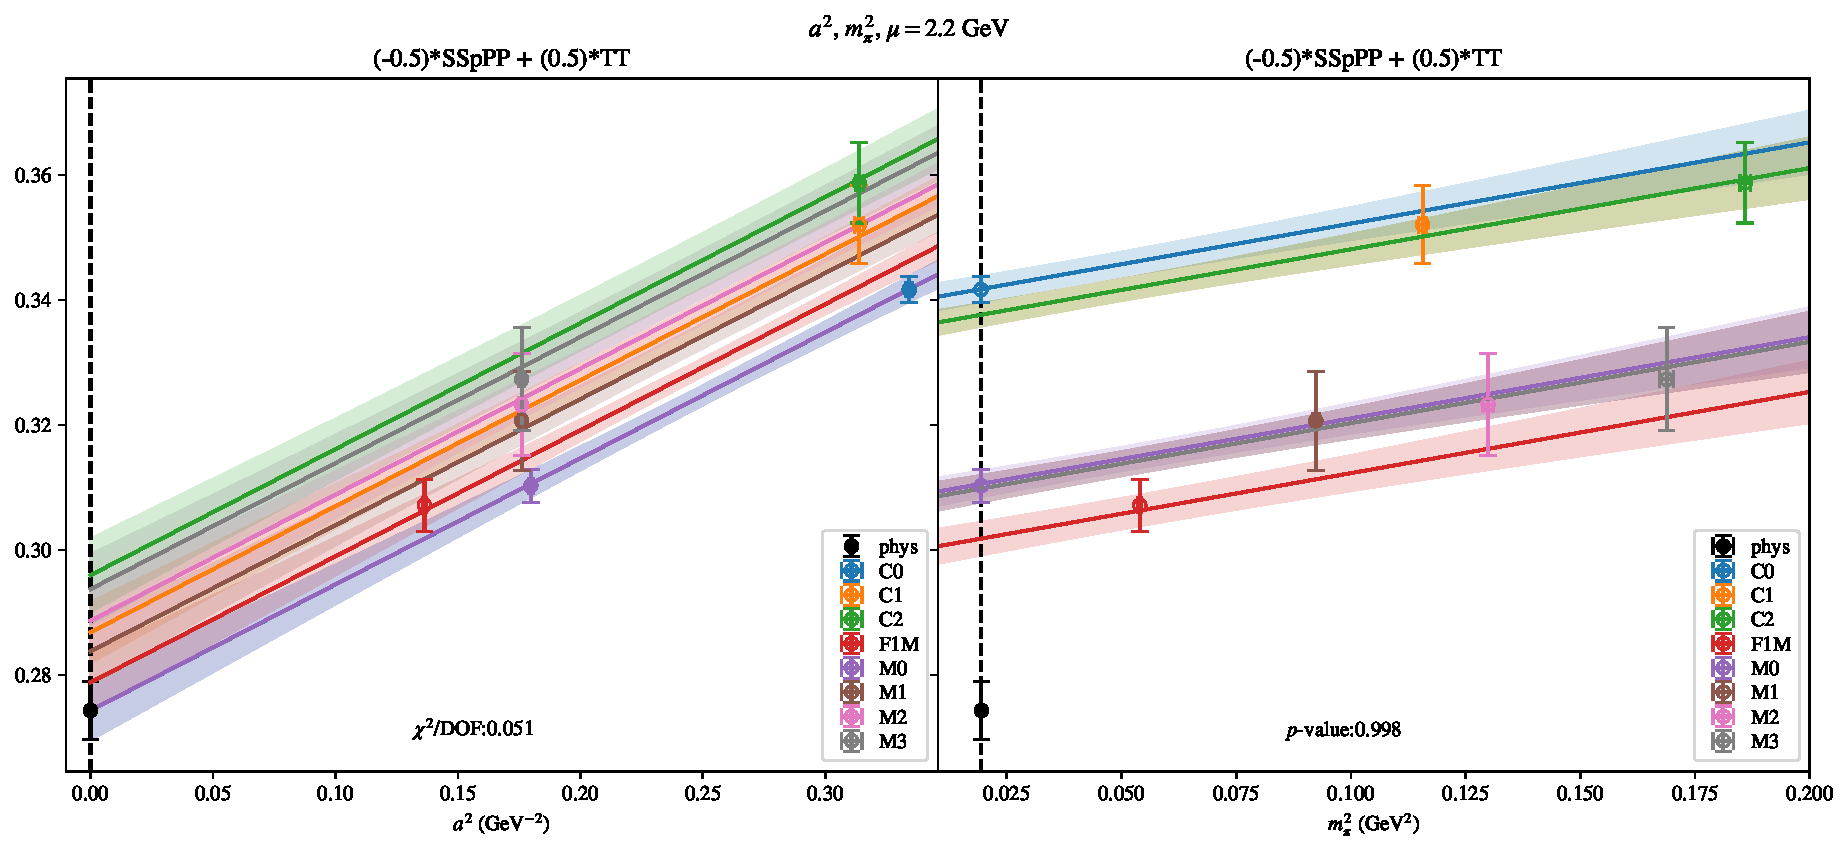
\includepdf[link, pages=-]{SSmPP/SUSY/bag_a2m2_22.pdf}
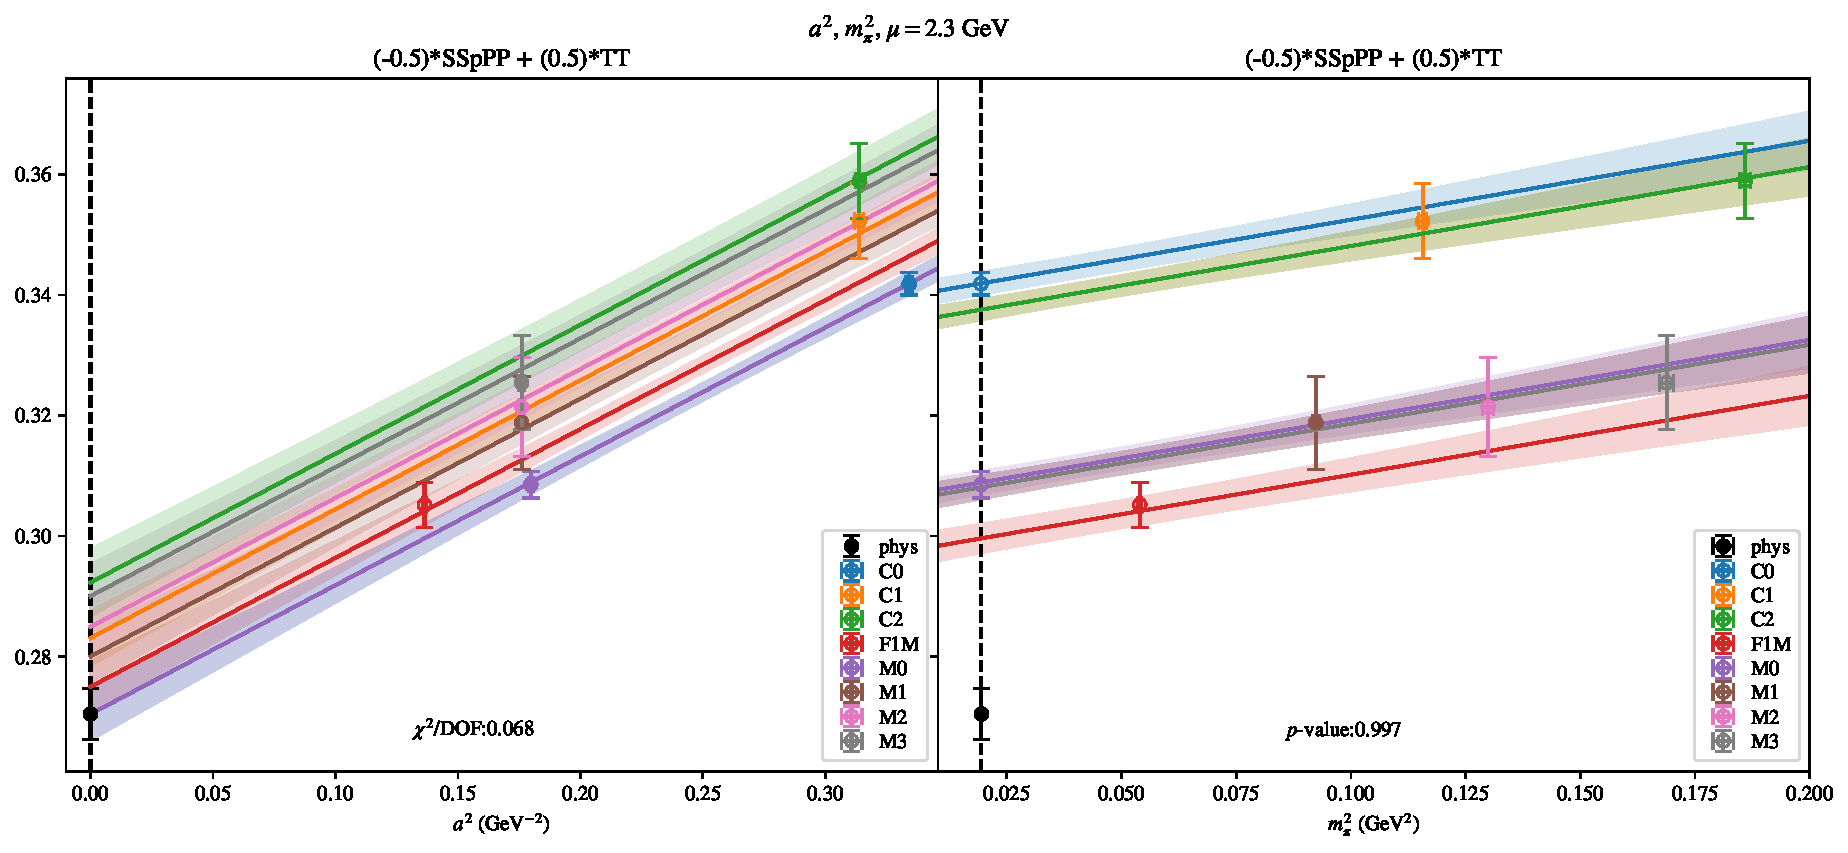
\includepdf[link, pages=-]{SSmPP/SUSY/bag_a2m2_23.pdf}
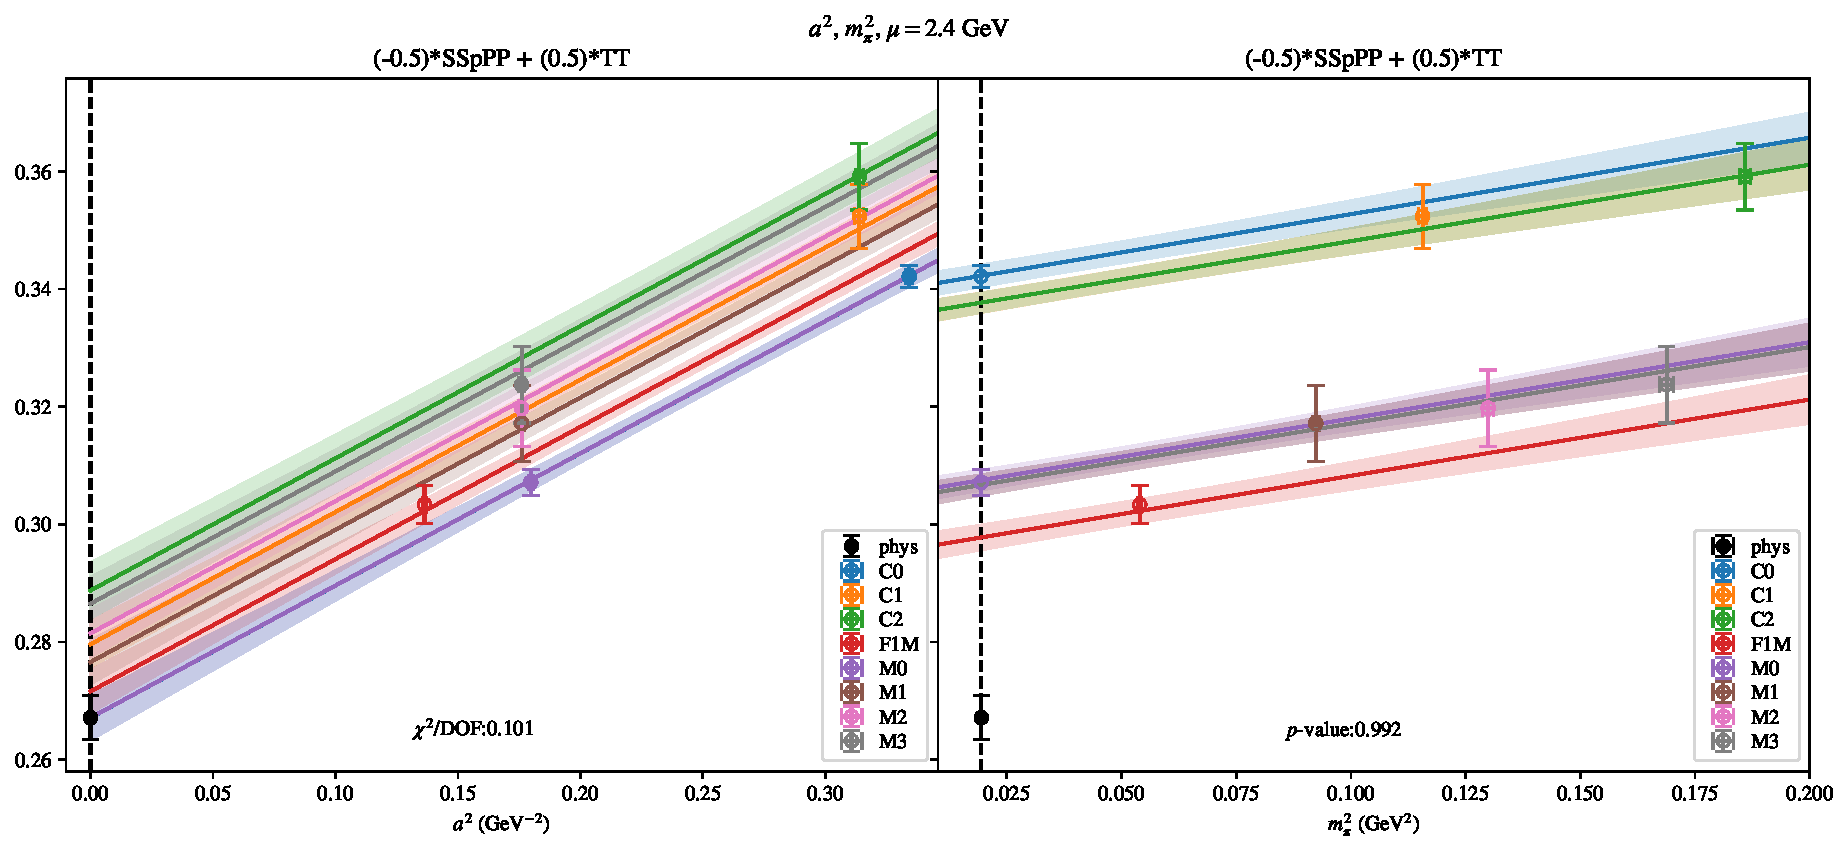
\includepdf[link, pages=-]{SSmPP/SUSY/bag_a2m2_24.pdf}
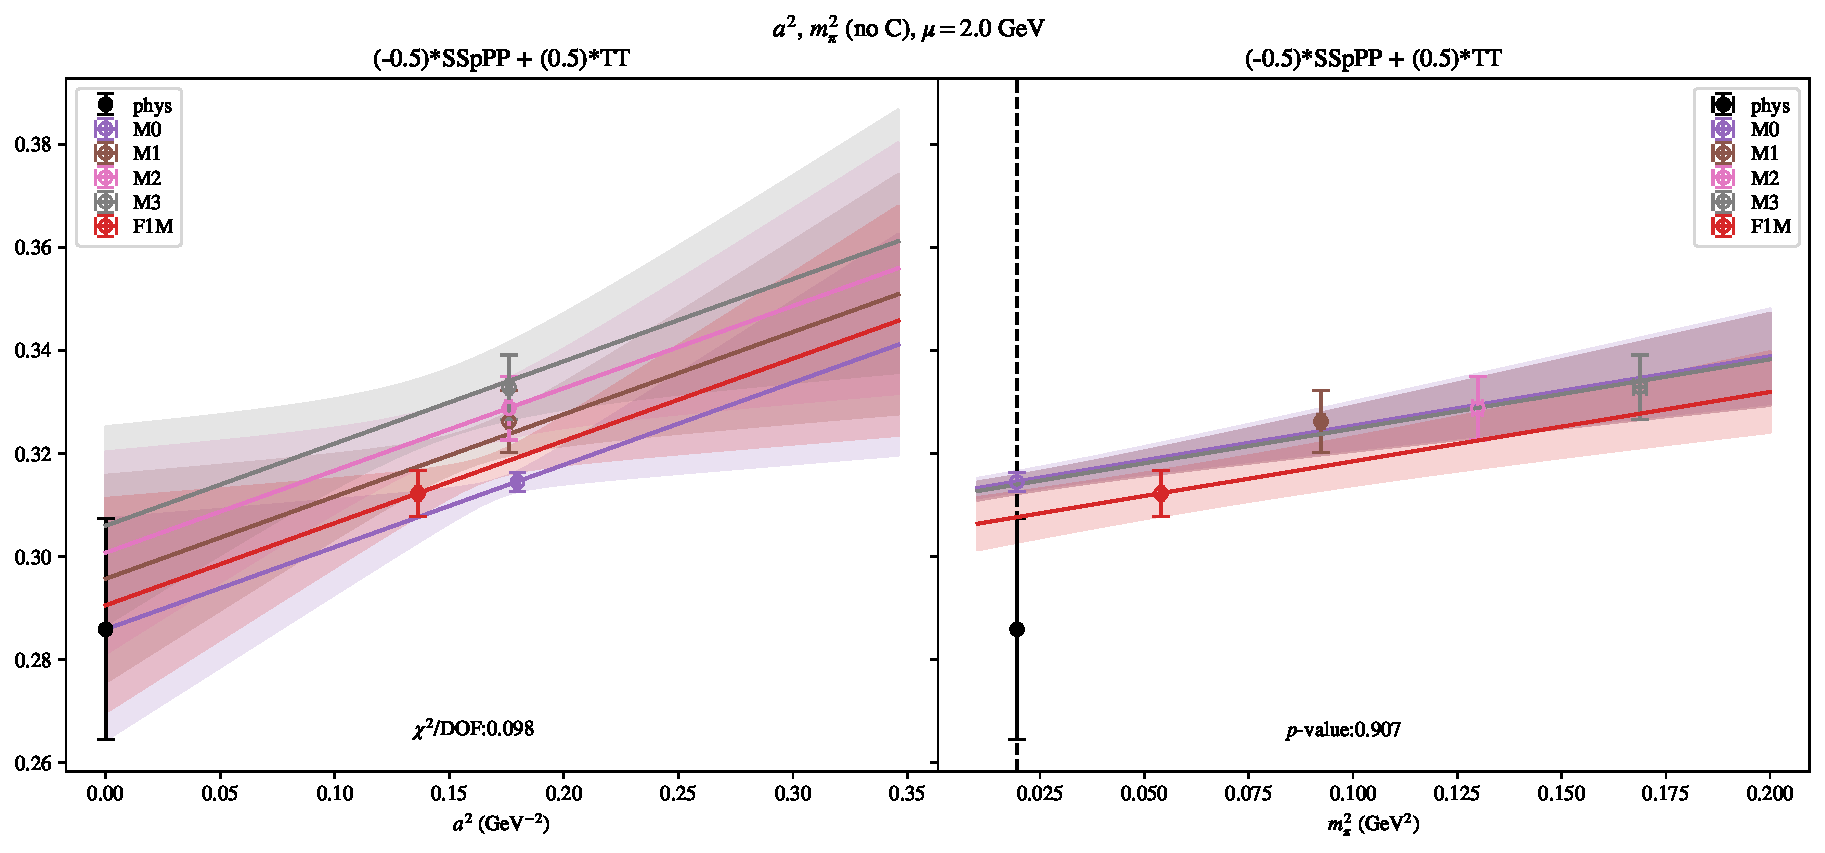
\includepdf[link, pages=-]{SSmPP/SUSY/bag_a2m2noC_20.pdf}
\includepdf[link, pages=-]{SSmPP/SUSY/bag_a2m2noC_22.pdf}
\includepdf[link, pages=-]{SSmPP/SUSY/bag_a2m2noC_23.pdf}
\includepdf[link, pages=-]{SSmPP/SUSY/bag_a2m2noC_24.pdf}
\includepdf[link, pages=-]{SSmPP/SUSY/bag_a2a4m2_20.pdf}
\includepdf[link, pages=-]{SSmPP/SUSY/bag_a2a4m2_22.pdf}
\includepdf[link, pages=-]{SSmPP/SUSY/bag_a2a4m2_23.pdf}
\includepdf[link, pages=-]{SSmPP/SUSY/bag_a2a4m2_24.pdf}
\includepdf[link, pages=-]{SSmPP/SUSY/bag_a2m2mcut_20.pdf}
\includepdf[link, pages=-]{SSmPP/SUSY/bag_a2m2mcut_22.pdf}
\includepdf[link, pages=-]{SSmPP/SUSY/bag_a2m2mcut_23.pdf}
\includepdf[link, pages=-]{SSmPP/SUSY/bag_a2m2mcut_24.pdf}
\includepdf[link, pages=-]{SSmPP/SUSY/bag_a2m2delm_20.pdf}
\includepdf[link, pages=-]{SSmPP/SUSY/bag_a2m2delm_22.pdf}
\includepdf[link, pages=-]{SSmPP/SUSY/bag_a2m2delm_23.pdf}
\includepdf[link, pages=-]{SSmPP/SUSY/bag_a2m2delm_24.pdf}
\clearpage
\section{$\mathcal{B}_4$}
\begin{table}[h!]
\begin{center}
\begin{tabular}{|c|c|c|c|c|c|}
\hline
$\mu$ (GeV) & $a^2$, $m_\pi^2$& $a^2$, $m_\pi^2$ (no C)& $a^2$, $m_\pi^2$, $a^4$& $a^2$, $m_\pi^2$ (no M3, C2)& $a^2$, $m_\pi^2$, $\delta m_s$\\
\hline
2.0& \hyperlink{SSpPP/SUSY/bag_a2m2_20.pdf.1}{\textbf{1.7955(44)}: 5.942 (0.0)} & \hyperlink{SSpPP/SUSY/bag_a2m2noC_20.pdf.1}{\textbf{1.703(17)}: 0.051 (0.95)} & \hyperlink{SSpPP/SUSY/bag_a2a4m2_20.pdf.1}{\textbf{1.650(28)}: 0.913 (0.455)} & \hyperlink{SSpPP/SUSY/bag_a2m2mcut_20.pdf.1}{\textbf{1.7960(47)}: 9.249 (0.0)} & \hyperlink{SSpPP/SUSY/bag_a2m2delm_20.pdf.1}{\textbf{1.7959(48)}: 2.461 (0.043)}\\
2.2& \hyperlink{SSpPP/SUSY/bag_a2m2_22.pdf.1}{\textbf{1.8013(36)}: 7.138 (0.0)} & \hyperlink{SSpPP/SUSY/bag_a2m2noC_22.pdf.1}{\textbf{1.717(14)}: 0.148 (0.862)} & \hyperlink{SSpPP/SUSY/bag_a2a4m2_22.pdf.1}{\textbf{1.666(25)}: 1.056 (0.376)} & \hyperlink{SSpPP/SUSY/bag_a2m2mcut_22.pdf.1}{\textbf{1.8021(39)}: 11.178 (0.0)} & \hyperlink{SSpPP/SUSY/bag_a2m2delm_22.pdf.1}{\textbf{1.8014(39)}: 4.119 (0.002)}\\
2.3& \hyperlink{SSpPP/SUSY/bag_a2m2_23.pdf.1}{\textbf{1.8036(35)}: 7.077 (0.0)} & \hyperlink{SSpPP/SUSY/bag_a2m2noC_23.pdf.1}{\textbf{1.721(14)}: 0.19 (0.827)} & \hyperlink{SSpPP/SUSY/bag_a2a4m2_23.pdf.1}{\textbf{1.667(24)}: 0.732 (0.57)} & \hyperlink{SSpPP/SUSY/bag_a2m2mcut_23.pdf.1}{\textbf{1.8045(38)}: 11.369 (0.0)} & \hyperlink{SSpPP/SUSY/bag_a2m2delm_23.pdf.1}{\textbf{1.8034(37)}: 3.989 (0.003)}\\
2.4& \hyperlink{SSpPP/SUSY/bag_a2m2_24.pdf.1}{\textbf{1.8052(33)}: 6.925 (0.0)} & \hyperlink{SSpPP/SUSY/bag_a2m2noC_24.pdf.1}{\textbf{1.726(14)}: 0.227 (0.797)} & \hyperlink{SSpPP/SUSY/bag_a2a4m2_24.pdf.1}{\textbf{1.675(24)}: 0.862 (0.486)} & \hyperlink{SSpPP/SUSY/bag_a2m2mcut_24.pdf.1}{\textbf{1.8058(37)}: 11.222 (0.0)} & \hyperlink{SSpPP/SUSY/bag_a2m2delm_24.pdf.1}{\textbf{1.8051(35)}: 4.387 (0.002)}\\
\hline
\end{tabular}
\caption{Physical point value from chiral and continuum extrapolation at renormalisation scale $\mu$. Entries are \textbf{value(error)}: $\chi^2/\text{DOF}$ ($p$-value).}
\end{center}
\end{table}
\begin{table}[h!]
\begin{center}
\begin{tabular}{|c c|c|c|c|c|c|}
\hline
$\mu$ (GeV) &  & $a^2$, $m_\pi^2$& $a^2$, $m_\pi^2$ (no C)& $a^2$, $m_\pi^2$, $a^4$& $a^2$, $m_\pi^2$ (no M3, C2)& $a^2$, $m_\pi^2$, $\delta m_s$\\
\hline
\multirow{3}{0.5in}{2.0} & $\alpha$ & 0.150(17)& 0.70(10)& 1.49(26)& 0.149(18)& 0.138(19)\\
 & $\beta$ & -0.00058(44)& 0.00016(80)& -0.00097(45)& -0.00126(74)& -0.00370(82)\\
 & $\gamma$ &  &  & -2.71(53)&  & 0.127(28)\\
\hline
\multirow{3}{0.5in}{2.2} & $\alpha$ & 0.150(13)& 0.653(86)& 1.39(22)& 0.148(14)& 0.142(14)\\
 & $\beta$ & -0.00070(30)& -0.00051(61)& -0.00125(32)& -0.00129(52)& -0.00322(65)\\
 & $\gamma$ &  &  & -2.53(46)&  & 0.100(22)\\
\hline
\multirow{3}{0.5in}{2.3} & $\alpha$ & 0.151(13)& 0.644(84)& 1.40(22)& 0.149(14)& 0.145(14)\\
 & $\beta$ & -0.00043(30)& -0.00049(58)& -0.00100(32)& -0.00087(49)& -0.00290(63)\\
 & $\gamma$ &  &  & -2.54(44)&  & 0.097(21)\\
\hline
\multirow{3}{0.5in}{2.4} & $\alpha$ & 0.154(12)& 0.627(82)& 1.35(21)& 0.153(13)& 0.147(13)\\
 & $\beta$ & -0.00034(27)& -0.00041(51)& -0.00089(29)& -0.00066(43)& -0.00249(59)\\
 & $\gamma$ &  &  & -2.43(44)&  & 0.085(20)\\
\hline
\end{tabular}
\caption{Fit values of coefficients in $Q = Q_{phys} + \mathbf{\alpha} a^2 + \mathbf{\beta}\left(\frac{m_\pi^2}{f_\pi^2}-\frac{m_{\pi,PDG}^2}{f_\pi^2}\right) + \gamma(\ldots)$}
\end{center}
\end{table}
\includepdf[link, pages=-]{SSpPP/SUSY/bag_a2m2_20.pdf}
\includepdf[link, pages=-]{SSpPP/SUSY/bag_a2m2_22.pdf}
\includepdf[link, pages=-]{SSpPP/SUSY/bag_a2m2_23.pdf}
\includepdf[link, pages=-]{SSpPP/SUSY/bag_a2m2_24.pdf}
\includepdf[link, pages=-]{SSpPP/SUSY/bag_a2m2noC_20.pdf}
\includepdf[link, pages=-]{SSpPP/SUSY/bag_a2m2noC_22.pdf}
\includepdf[link, pages=-]{SSpPP/SUSY/bag_a2m2noC_23.pdf}
\includepdf[link, pages=-]{SSpPP/SUSY/bag_a2m2noC_24.pdf}
\includepdf[link, pages=-]{SSpPP/SUSY/bag_a2a4m2_20.pdf}
\includepdf[link, pages=-]{SSpPP/SUSY/bag_a2a4m2_22.pdf}
\includepdf[link, pages=-]{SSpPP/SUSY/bag_a2a4m2_23.pdf}
\includepdf[link, pages=-]{SSpPP/SUSY/bag_a2a4m2_24.pdf}
\includepdf[link, pages=-]{SSpPP/SUSY/bag_a2m2mcut_20.pdf}
\includepdf[link, pages=-]{SSpPP/SUSY/bag_a2m2mcut_22.pdf}
\includepdf[link, pages=-]{SSpPP/SUSY/bag_a2m2mcut_23.pdf}
\includepdf[link, pages=-]{SSpPP/SUSY/bag_a2m2mcut_24.pdf}
\includepdf[link, pages=-]{SSpPP/SUSY/bag_a2m2delm_20.pdf}
\includepdf[link, pages=-]{SSpPP/SUSY/bag_a2m2delm_22.pdf}
\includepdf[link, pages=-]{SSpPP/SUSY/bag_a2m2delm_23.pdf}
\includepdf[link, pages=-]{SSpPP/SUSY/bag_a2m2delm_24.pdf}
\clearpage
\section{$\mathcal{B}_5$}
\begin{table}[h!]
\begin{center}
\begin{tabular}{|c|c|c|c|c|c|}
\hline
$\mu$ (GeV) & $a^2$, $m_\pi^2$& $a^2$, $m_\pi^2$ (no C)& $a^2$, $m_\pi^2$, $a^4$& $a^2$, $m_\pi^2$ (no M3, C2)& $a^2$, $m_\pi^2$, $\delta m_s$\\
\hline
2.0& \hyperlink{TT/SUSY/bag_a2m2_20.pdf.1}{\textbf{0.4933(62)}: 0.162 (0.976)} & \hyperlink{TT/SUSY/bag_a2m2noC_20.pdf.1}{\textbf{0.471(25)}: 0.003 (0.997)} & \hyperlink{TT/SUSY/bag_a2a4m2_20.pdf.1}{\textbf{0.459(42)}: 0.04 (0.997)} & \hyperlink{TT/SUSY/bag_a2m2mcut_20.pdf.1}{\textbf{0.4934(65)}: 0.248 (0.863)} & \hyperlink{TT/SUSY/bag_a2m2delm_20.pdf.1}{\textbf{0.4933(62)}: 0.09 (0.986)}\\
2.2& \hyperlink{TT/SUSY/bag_a2m2_22.pdf.1}{\textbf{0.5004(49)}: 0.196 (0.964)} & \hyperlink{TT/SUSY/bag_a2m2noC_22.pdf.1}{\textbf{0.481(20)}: 0.008 (0.992)} & \hyperlink{TT/SUSY/bag_a2a4m2_22.pdf.1}{\textbf{0.469(34)}: 0.031 (0.998)} & \hyperlink{TT/SUSY/bag_a2m2mcut_22.pdf.1}{\textbf{0.5008(52)}: 0.292 (0.831)} & \hyperlink{TT/SUSY/bag_a2m2delm_22.pdf.1}{\textbf{0.5003(49)}: 0.114 (0.978)}\\
2.3& \hyperlink{TT/SUSY/bag_a2m2_23.pdf.1}{\textbf{0.5038(44)}: 0.24 (0.945)} & \hyperlink{TT/SUSY/bag_a2m2noC_23.pdf.1}{\textbf{0.484(20)}: 0.009 (0.991)} & \hyperlink{TT/SUSY/bag_a2a4m2_23.pdf.1}{\textbf{0.470(32)}: 0.02 (0.999)} & \hyperlink{TT/SUSY/bag_a2m2mcut_23.pdf.1}{\textbf{0.5042(47)}: 0.365 (0.779)} & \hyperlink{TT/SUSY/bag_a2m2delm_23.pdf.1}{\textbf{0.5035(45)}: 0.119 (0.976)}\\
2.4& \hyperlink{TT/SUSY/bag_a2m2_24.pdf.1}{\textbf{0.5056(42)}: 0.257 (0.937)} & \hyperlink{TT/SUSY/bag_a2m2noC_24.pdf.1}{\textbf{0.487(17)}: 0.009 (0.991)} & \hyperlink{TT/SUSY/bag_a2a4m2_24.pdf.1}{\textbf{0.474(29)}: 0.025 (0.999)} & \hyperlink{TT/SUSY/bag_a2m2mcut_24.pdf.1}{\textbf{0.5060(46)}: 0.398 (0.754)} & \hyperlink{TT/SUSY/bag_a2m2delm_24.pdf.1}{\textbf{0.5057(42)}: 0.13 (0.971)}\\
\hline
\end{tabular}
\caption{Physical point value from chiral and continuum extrapolation at renormalisation scale $\mu$. Entries are \textbf{value(error)}: $\chi^2/\text{DOF}$ ($p$-value).}
\end{center}
\end{table}
\begin{table}[h!]
\begin{center}
\begin{tabular}{|c c|c|c|c|c|c|}
\hline
$\mu$ (GeV) &  & $a^2$, $m_\pi^2$& $a^2$, $m_\pi^2$ (no C)& $a^2$, $m_\pi^2$, $a^4$& $a^2$, $m_\pi^2$ (no M3, C2)& $a^2$, $m_\pi^2$, $\delta m_s$\\
\hline
\multirow{3}{0.5in}{2.0} & $\alpha$ & -0.080(22)& 0.05(14)& 0.23(38)& -0.080(23)& -0.081(22)\\
 & $\beta$ & 0.00093(63)& 0.0011(11)& 0.00082(64)& 0.0008(10)& 0.0002(11)\\
 & $\gamma$ &  &  & -0.63(77)&  & 0.027(38)\\
\hline
\multirow{3}{0.5in}{2.2} & $\alpha$ & -0.104(17)& 0.01(11)& 0.19(31)& -0.105(18)& -0.105(17)\\
 & $\beta$ & 0.00078(51)& 0.00082(88)& 0.00068(52)& 0.00057(83)& 0.00018(99)\\
 & $\gamma$ &  &  & -0.58(63)&  & 0.024(31)\\
\hline
\multirow{3}{0.5in}{2.3} & $\alpha$ & -0.117(16)& 0.002(114)& 0.19(29)& -0.118(17)& -0.118(16)\\
 & $\beta$ & 0.00084(46)& 0.00082(79)& 0.00074(47)& 0.00063(78)& 0.00019(86)\\
 & $\gamma$ &  &  & -0.62(58)&  & 0.026(29)\\
\hline
\multirow{3}{0.5in}{2.4} & $\alpha$ & -0.126(15)& -0.02(10)& 0.16(26)& -0.127(16)& -0.128(15)\\
 & $\beta$ & 0.00087(42)& 0.00084(71)& 0.00075(43)& 0.00069(72)& 0.00025(81)\\
 & $\gamma$ &  &  & -0.58(54)&  & 0.024(27)\\
\hline
\end{tabular}
\caption{Fit values of coefficients in $Q = Q_{phys} + \mathbf{\alpha} a^2 + \mathbf{\beta}\left(\frac{m_\pi^2}{f_\pi^2}-\frac{m_{\pi,PDG}^2}{f_\pi^2}\right) + \gamma(\ldots)$}
\end{center}
\end{table}
\includepdf[link, pages=-]{TT/SUSY/bag_a2m2_20.pdf}
\includepdf[link, pages=-]{TT/SUSY/bag_a2m2_22.pdf}
\includepdf[link, pages=-]{TT/SUSY/bag_a2m2_23.pdf}
\includepdf[link, pages=-]{TT/SUSY/bag_a2m2_24.pdf}
\includepdf[link, pages=-]{TT/SUSY/bag_a2m2noC_20.pdf}
\includepdf[link, pages=-]{TT/SUSY/bag_a2m2noC_22.pdf}
\includepdf[link, pages=-]{TT/SUSY/bag_a2m2noC_23.pdf}
\includepdf[link, pages=-]{TT/SUSY/bag_a2m2noC_24.pdf}
\includepdf[link, pages=-]{TT/SUSY/bag_a2a4m2_20.pdf}
\includepdf[link, pages=-]{TT/SUSY/bag_a2a4m2_22.pdf}
\includepdf[link, pages=-]{TT/SUSY/bag_a2a4m2_23.pdf}
\includepdf[link, pages=-]{TT/SUSY/bag_a2a4m2_24.pdf}
\includepdf[link, pages=-]{TT/SUSY/bag_a2m2mcut_20.pdf}
\includepdf[link, pages=-]{TT/SUSY/bag_a2m2mcut_22.pdf}
\includepdf[link, pages=-]{TT/SUSY/bag_a2m2mcut_23.pdf}
\includepdf[link, pages=-]{TT/SUSY/bag_a2m2mcut_24.pdf}
\includepdf[link, pages=-]{TT/SUSY/bag_a2m2delm_20.pdf}
\includepdf[link, pages=-]{TT/SUSY/bag_a2m2delm_22.pdf}
\includepdf[link, pages=-]{TT/SUSY/bag_a2m2delm_23.pdf}
\includepdf[link, pages=-]{TT/SUSY/bag_a2m2delm_24.pdf}
\clearpage
\end{document}